%----------------------------------------------------------------%
%--------------------------INFORMATIONEN-------------------------%
%----------------------------------------------------------------%
%	Infos gibt es zu jedem Paket auf www.ctan.org
%	Werden bei den Paketen bestimmte Optionen gesetzt, so sind die Wichtigsten erklaert
%	solange sie nicht selbsterklärend sind

%----------------------------------------------------------------%
%--------------------------GRUNDEINSTELLUNGEN--------------------%
%----------------------------------------------------------------%
%\documentclass[oneside, ngerman]{scrartcl}
\documentclass[oneside, english]{scrartcl}
%	'oneside'/'twoside': nicht zwischen linker und rechter Seite unterscheiden (alternativ twoside)
%	'twocolumn': wuerde 2 Spalten auf dem Blatt platzieren
%	'bibliography=totocnumbered': Normal nummeriertes Inhaltsverzeichnis (Kapitelnummer)
%	'listof=totocnumbered': Abbildungs- und Tabellenverzeichnis normal nummeriert (Kapitelnummer)
%	'ngerman' verwendet deutsch als Dokumentensprache (z.B. fuer Sirange)

\usepackage[english,ngerman]{babel}							%	Einstellen der Sprache
\usepackage[T1]{fontenc}							%	Wie wird Text ausgegeben, d.h. im PDF
\usepackage[utf8]{inputenc}							%	Welche Zeichen 'versteht' LaTeX bei der Eingabe?
\usepackage{lmodern}								%	Laedt Schriften, die geglaettet sind
											
\usepackage{blindtext}								%	Beispieltext, zum Testen geeignet
\usepackage{subfigure}
%----------------------------------------------------------------%
%--------------------------SEITENLAYOUT--------------------------%
%----------------------------------------------------------------%
\usepackage[left=3cm,right=3cm]{geometry}			%	Paket, welches vielfaeltige Einstellungen zum Seitenlayout liefert

%----------------------------------------------------------------%
%--------------------------ABSTÄNDE------------------------------%
%----------------------------------------------------------------%
\usepackage[onehalfspacing]{setspace}				%	Für Zeilenabstaende: 'singlespacing' (einfach), 'onehalfspacing' (1.5-fach), 'doublespacing' (2fach)

%\setlength{\parindent}{0cm}						%	Laengenangabe für die Einrueckung der ersten Zeile eines neuen Absatzes.
%\setlength{\parskip}{6pt plus 3pt minus 3pt}		%	Laengenangabe für den Abstand zwischen zwei Absaetzen.
%	Wenn diese beiden Befehle nicht kommentiert sind, wird ein Absatz nicht eingezogen sondern es gibt einen Abstand

%----------------------------------------------------------------%
%--------------------------MATHE---------------------------------%
%----------------------------------------------------------------%
\usepackage[]{mathtools}							%	Erweiterung von AMSMath, laedt automatisch AMSMath - für viele Mathe-Werkzeuge, 'fleqn' als Option ist für Mathe linksbuendig
\usepackage{amsfonts}								%	Für eine Vielzahl an mathematischen Symbolen

%----------------------------------------------------------------%
%--------------------------KOPF- UND FUSSZEILEN------------------%
%----------------------------------------------------------------%
\usepackage[automark,headsepline=.4pt]{scrlayer-scrpage}
\pagestyle{scrheadings}
\setkomafont{pageheadfoot}{\normalfont\bfseries}	%	Normale Schriftart und Fett für den Seitenkopf
\addtokomafont{pagenumber}{\normalfont\bfseries}	%	Normale Schriftart und Fett für die Seitenzahl
\clearscrheadfoot
\rohead{\thepage}									%	Rechter Seitenkopf mit Seitenzahl, ungerade Seiten
\lehead{\thepage}									%	Linker Seitenkopf mit Seitenzahl, gerade Seiten
\lohead{\headmark}									%	Linker Seitenkopf mit section, ungerade Seiten
\rehead{\headmark}									%	Linker Seitenkopf mit section, gerade Seiten
\lefoot[\pagemark]{\empty}							%	Leere Fußzeile, ungerade Seiten
\rofoot[\pagemark]{\empty}							%	Leere Fußzeile, gerade Seiten
\setlength{\headheight}{1.1\baselineskip}			%	Hoehe der Kopfzeile definieren
%	Definert man oben in der documentclass 'twoside', so wird zwischen geraden und ungeraden Seiten unterschieden

%----------------------------------------------------------------%
%--------------------------BILDER--------------------------------%
%----------------------------------------------------------------%
\usepackage{graphicx}									%	Um Bilder einbinden zu koennen
\usepackage[usenames,dvipsnames,svgnames]{xcolor}		%	Um Farben verwenden zu koennen
\usepackage{pdfpages}									%	pdfs importieren

%----------------------------------------------------------------%
%--------------------------POSITIONIERUNG------------------------%
%----------------------------------------------------------------%
\usepackage{float}

%----------------------------------------------------------------%
%--------------------------LISTEN--------------------------------%
%----------------------------------------------------------------%
\usepackage{enumitem}							%	Um Listen / Aufzaehlungen leichter zu modifizieren
%\setlist{noitemsep}							%	Verringert den Abstand in Aufzaehlungen

%----------------------------------------------------------------%
%--------TABELLEN-/BILDUNTERSCHRIFTEN und NUMMERIERUNG-----------%
%----------------------------------------------------------------%
\usepackage[format=hang, indention=0mm, labelsep=colon, justification=justified,  labelfont=bf]{caption}
\setlength\parindent{0pt}
%	'format=hang': Platz unter Abb. X bleibt frei, 'format=plain': auch unter Abb. X befindet sich Text
%	'idention': Einzug der zweiten Textzeile
%	'labelsep=colon': Trenner zwischen Nr. und Text ist Doppelpunkt und Leerzeichen
%	'justification=justified': Text wird als Block gesetzt
%	'labelfont=bf': 'Abbildung X.X' wird fett geschrieben

\numberwithin{equation}{section}				%	Nummerierung der Gleichungen, Tabellen und Bilder nach der Kapitelnummer
\numberwithin{figure}{section}
\numberwithin{table}{section}

%----------------------------------------------------------------%
%--------------------------LITERATURVERZEICHNIS------------------%
%----------------------------------------------------------------%
\usepackage[german]{babelbib}					%	Bereitstellung des deutschen Layouts fuer die Bibliography

%----------------------------------------------------------------%
%--------------------------SIUNITX-------------------------------%
%----------------------------------------------------------------%
\usepackage[]{siunitx}
\sisetup{locale = DE}							%	Automatische Einstellung der Ausgabe für bestimmte Regionen (UK, US, DE, FR, ZA)

%----------------------------------------------------------------%
%--------------------------URLs / REFs---------------------------%
%----------------------------------------------------------------%
\usepackage[hidelinks]{hyperref}				%	Erweiterte Referenzierung ('hidelinks' verhindert Linien um Links)
\usepackage{gensymb}
\usepackage{subfigure}
\usepackage{ textcomp }
\usepackage{dsfont}
\usepackage{siunitx}
\usepackage{comment}
\usepackage{tikz}
\usepackage{epstopdf}
\usepackage{graphicx}
\usetikzlibrary{arrows.meta}
%----------------------------------------------------------------%
%--------------------------EIGENE BEFEHLE------------------------%
%----------------------------------------------------------------%
\DeclareSIUnit\parsec{pc}                               %   Neuer SI-Command Parsec
\DeclareSIUnit\lightyear{ly}                            %   Neuer SI-Command Lichtjahr
\newcommand{\textSC}[1]{{\normalfont \textsc{#1}}}      %   Für Kapitälchen in Überschriften
\DeclareMathOperator{\sinc}{sinc}                       %   sinc-Funktion

\begin{document}
\selectlanguage{english}
%----------------------------------------------------------------%
%----------------------Titelseite--------------------------------%
%----------------------------------------------------------------%
% !TEX root = main.tex
\title{Earths-Field-NMR Remote}
\subtitle{Physikalisches Fortgeschrittenenpraktikum at University of Constance}
\author{Authors: Philipp Gebauer, Simon Keegan and Marc Neumann \\ \large{Tutors: Narinder Narinder and Matthias Falk}}
\date{Execution on 9th of July 2020 and \textcolor{red}{???}}
\maketitle
\begin{abstract}
    \begin{center}
        \Large{\textsf{\textbf{Abstract}}}
    \end{center}
    \vspace{0.75 cm}
    \begin{singlespace}
    \noindent The aim of this paper is to show the principals of an EFNMR measurement and to discuss its results.\newline
    The first part of the experiment is about the basic principal of an EFNMR measurement. Therefore the noise level is taken into account and is identified to be \SI{7.5}{\mu \volt} for our setup. In order to tune the circuit to the lamor frequency of \SI{1841.4}{\hertz}, the LCR circuit in the B$_1$ coil has to have a capacity of \SI{13.8}{\nano \farad}. To obtain a sharp peak in the spectrum of the measured hydrogen signal the system was tuned to following values: shimming values $x = \SI{10.11}{\milli \ampere}, \ y = \SI{20.88}{\milli \ampere}, \ z = \SI{-20.07}{\milli \ampere}$; B$_1$ pulse duration \SI{1.35}{\milli \second}; capacity \SI{13.8}{\nano \farad}. The relaxation time measurements in the polarizing field results in values for T$_{1,p}$ of \SI{2912.8800 \pm 0.0048}{\milli \second}. The relaxation time measurements in the earths magnetic field results in values for T$_{1,e}$ of \SI{2753.0500 \pm 0.0012}{\milli \second}. The measurements of T$_2$ results in values of \SI{2691 \pm 12}{\milli \second} with single \textit{Hahn} echos and \SI{2317.76000 \pm 0.00062}{\milli \second} with the use of 30 echos in a CPMG.
    \vspace{0.75 cm}
     
    \noindent All authors have worked equally on all parts of this paper and used no other sources than listed in the bibliography.

\end{singlespace}
\end{abstract}

\thispagestyle{empty}
\newpage
%----------------------------------------------------------------%
%----------------------Inhaltsverzeichnis------------------------%
%----------------------------------------------------------------%
\tableofcontents
\thispagestyle{empty}
\newpage
\setcounter{page}{1} 
%---------------------------------------------------------------%
%----------------------Einleitung--------------------------------%
%----------------------------------------------------------------%
% !TEX root = main.tex
\section{Introduction}
\label{sec:Introduction}
Earths field nuclear magnetic resonance is a widely used method in the quality management or in medical technology to gain knowledge about the structure of materials. Therefore the magnetic moment of spins is taken into account.\newline
Due to the external magnetic field of the earth B$_0$ (sometimes refered to B$_e$) the spins of hydrogen (spin quantum number: $I=\frac{1}{2}$) align either parallel or antiparallel to this magnetic field. Using the \textit{Boltzmann} statistics it can be calculated, if the spins are aligned parallel or antiparallel. Therefore the information about the temperature and the surrounding magnetic field B$_0$ is necessary. Each spin precesses around the surrounding magnetic field B$_0$ (along z-axis), most of the time in the spin up direction, because it is energetically more favorable. This precession evokes a component of the spins in the transversal plane. However, since the phase of the precession is random the net magentisation is aligned along the z-axis. By changing the properties of the surrounding magnetic field, the bulk magnetisation vector can be manipulated. In order to do so an alternating electro magnetic field pulse is applied. The frequency of this magnetic field (B$_1$) is in the radio frequency (RF) magnitude for large B$_0$ and for low B$_0$ it is in the ultra low frequency (ULF). Since we use the earths magnetic field B$_0$ for our measurements, the frequency is in the ULF magnitude. When the frequency of this magnetic field pulse is chosen right at the lamor frequency of the sample, the transitions between the energy levels of spin up and down happen more likely and therefore a phase coherence of the spins occurs. The applied pulse results in changing the spins direction by a tipping angle $\Theta$ from the vertical to the transversal plane. The precession of the spins can be measured in the transversal plane by a coil (B$_1$ coil) which is aligned orthogonal to the earths magnetic field. The B$_1$ coil is therefore the exciting and detecting coil and therefore the heart of our measurements. \\
The first part of this experiment is about the basics of ENMR. At first we have a look at the noise that is dependent on surrounding metal objects. Then we analyse the B$_1$ coil by changing the capacity of the LCR circuit. The next step is the optimization and characterisation of a free induction decay (FID) of a water sample. The aim of this chapter is to measure a sharp peak at the lamor frequency of the hydrogen in the water. When this is done the longitudinal relaxation time T$_1$ and the transversal relaxation time T$_2$ are measured and discussed.

%----------------------------------------------------------------%
%----------------------Grundlagen--------------------------------%
%----------------------------------------------------------------%

%----------------------------------------------------------------%
%-----------------------Aufbau und Durchführung------------------%
%---------------------------------------------------------------%
% !TEX root = main.tex
\section{Setup}
\label{sec:Aufbau}
This chapter is about the setup and execution process of this experiment. To understand which part of the experiment has what use, it is necessary to have a look at the components of the setup.\newline
Figure \ref{fig:Aufbau} shows the different coils which are necessary for the EFNMR measurement. The innerst coil B$_1$ coil is the excite and collect coil which is described in the previous chapter. The outer coil is to prepolarize the sample. This is necessary to obtain a stronger signal. By applying a strong magnetic field orthogonal to the earths magnetic field the spins align in the direction of the prepolarizing pulse and provides a bulk polarized nuclear magnetization across the sample. The middle coil is the gradient coil. This coil erases the inhomogenious magnetic field which always occurs for different uncertainty reasons. This coil is also used for the 2D imaging of the probe by adjusting the components of the magnetic field. Via the computer program \textit{Prospa} and the spectrometer the currents of the coil can be adjust and the induced signals can be measured.
\begin{figure}[H]
    \centering
    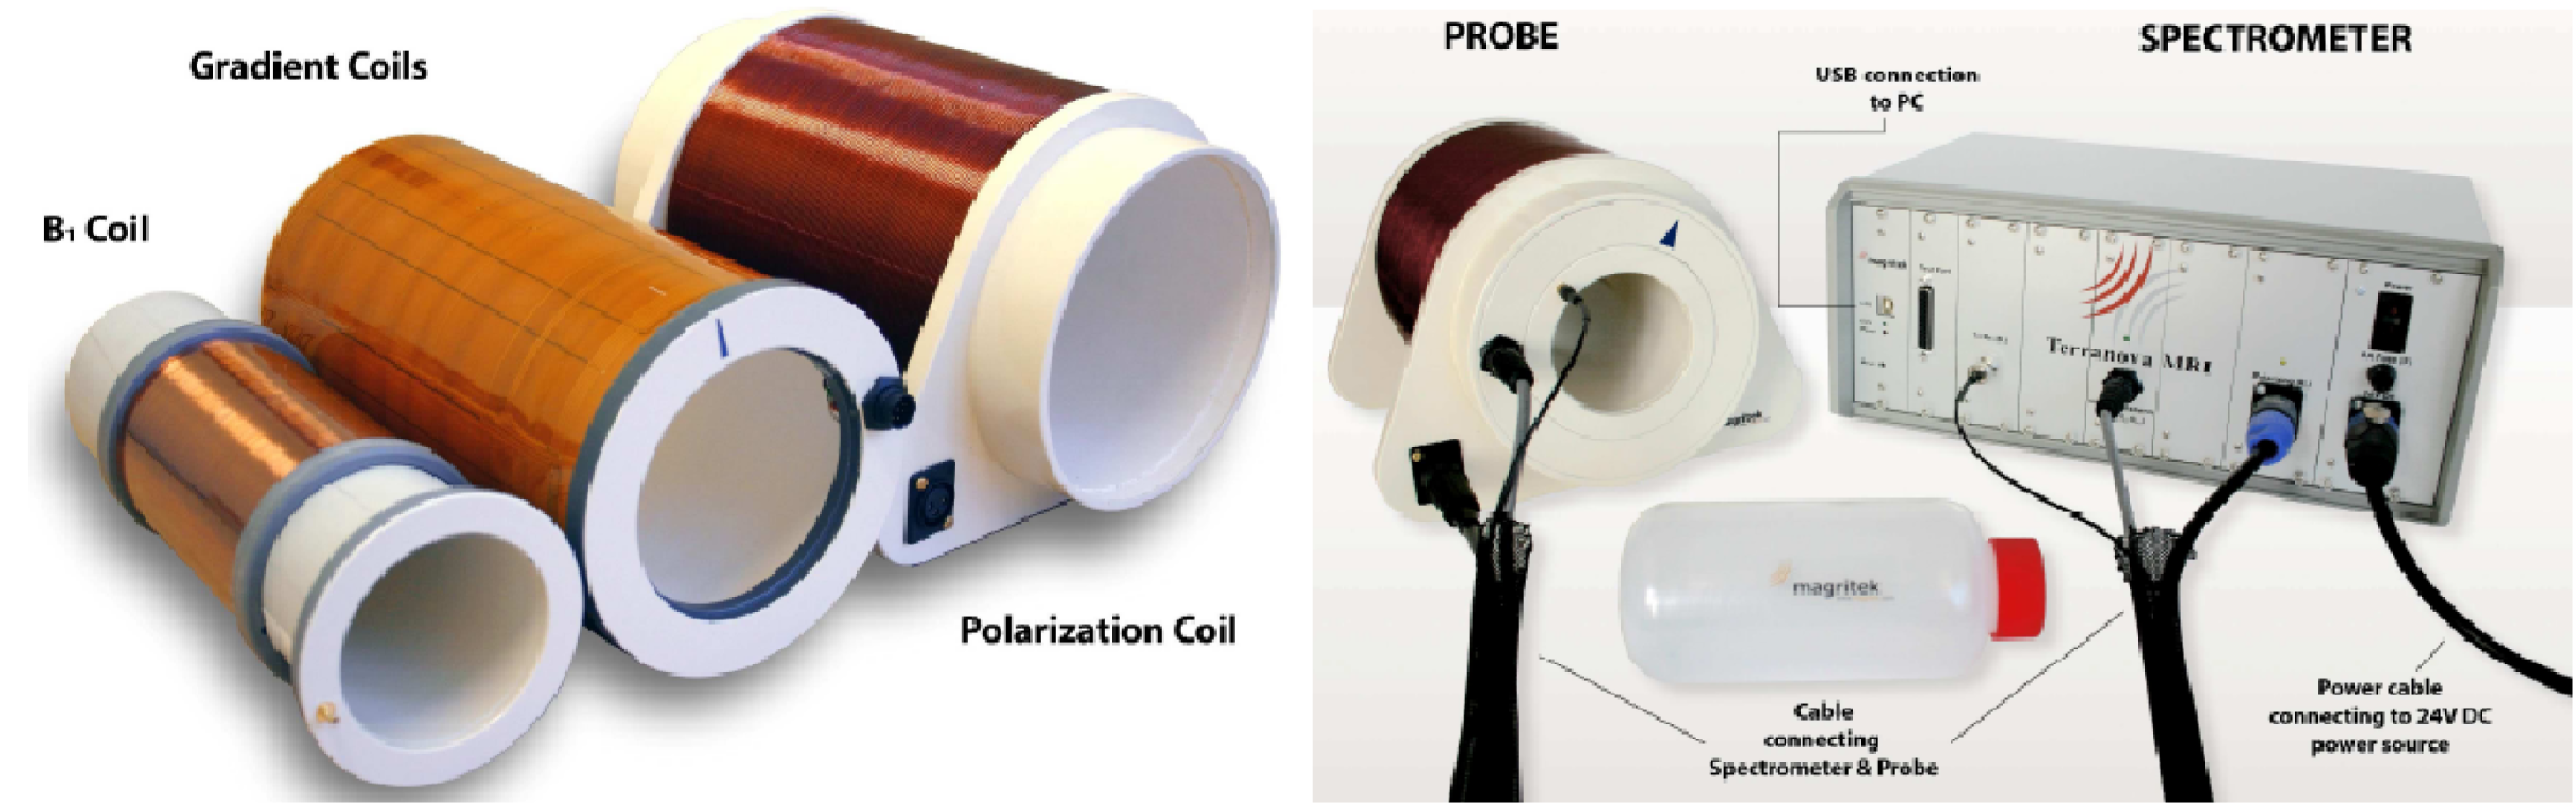
\includegraphics[width= \textwidth]{Aufbau.png}   
    \caption[Setup of the \textit{Terranova-MRI EFNMR}. \cite{Bild}]{Setup of the \textit{Terranova-MRI EFNMR}. On the left handside the coils B$_1$ (excite and collect coil), gradient coil (homogenious magnetic field and 2D scanning coil) and the prepolarizing coil B$_p$ are seen. The right hand side shows the water sample which has been used and the spectrometer which adjusts the right signals to the coils. \cite{Bild}}
    \label{fig:Aufbau}
\end{figure}

% !!!!!!!!
% !!!!!!!!!!
% !!!!!!!!!
% %Einstellen von größe des Bidles mit epslatex:  \resizebox{0.5\textwidth}{!}{\input{plots/Belichtungszeit.tex}}
% !!!!!!!!!!
% !!!!!!!!!!!
% !!!!!!!!!
\newpage
%----------------------------------------------------------------%
%----------------------Auswertung--------------------------------%
%----------------------------------------------------------------%
% !TEX root = main.tex
\section{Noisemeasurement}
% \label{sec:Noisemeasurement}
The first step in the EFNMR Remote experiment is to measure the external noise. The external noise depends on the location where the setup is placed, the orientation of the probe and by surrounding metal objects e.g. a metal desk. To detect this external noise, a measurement without an NMR signal is provided. The time domain noise signal is shwon in figure \ref{fig: noise}. It is clearly visible that the noise is centered around \SI{0}{\mu \volt}. To gain knowledge about the noise level, the computer calculates the root-mean-square (RMS). This means that it calculates the square of each data point, than sum up all squared values up, calculates the average and than applies a square root. With this method the noise level can be calulated. In this case it is \SI{7.5}{\mu \volt}. This is an ecceptable noise value, because any value below \SI{10}{\mu \volt} is good enough to provide good NMR data.

\begin{figure}[H]
    \centering
    % GNUPLOT: LaTeX picture with Postscript
\begingroup
  % Encoding inside the plot.  In the header of your document, this encoding
  % should to defined, e.g., by using
  % \usepackage[cp1252,<other encodings>]{inputenc}
  \inputencoding{cp1252}%
  \makeatletter
  \providecommand\color[2][]{%
    \GenericError{(gnuplot) \space\space\space\@spaces}{%
      Package color not loaded in conjunction with
      terminal option `colourtext'%
    }{See the gnuplot documentation for explanation.%
    }{Either use 'blacktext' in gnuplot or load the package
      color.sty in LaTeX.}%
    \renewcommand\color[2][]{}%
  }%
  \providecommand\includegraphics[2][]{%
    \GenericError{(gnuplot) \space\space\space\@spaces}{%
      Package graphicx or graphics not loaded%
    }{See the gnuplot documentation for explanation.%
    }{The gnuplot epslatex terminal needs graphicx.sty or graphics.sty.}%
    \renewcommand\includegraphics[2][]{}%
  }%
  \providecommand\rotatebox[2]{#2}%
  \@ifundefined{ifGPcolor}{%
    \newif\ifGPcolor
    \GPcolorfalse
  }{}%
  \@ifundefined{ifGPblacktext}{%
    \newif\ifGPblacktext
    \GPblacktexttrue
  }{}%
  % define a \g@addto@macro without @ in the name:
  \let\gplgaddtomacro\g@addto@macro
  % define empty templates for all commands taking text:
  \gdef\gplbacktext{}%
  \gdef\gplfronttext{}%
  \makeatother
  \ifGPblacktext
    % no textcolor at all
    \def\colorrgb#1{}%
    \def\colorgray#1{}%
  \else
    % gray or color?
    \ifGPcolor
      \def\colorrgb#1{\color[rgb]{#1}}%
      \def\colorgray#1{\color[gray]{#1}}%
      \expandafter\def\csname LTw\endcsname{\color{white}}%
      \expandafter\def\csname LTb\endcsname{\color{black}}%
      \expandafter\def\csname LTa\endcsname{\color{black}}%
      \expandafter\def\csname LT0\endcsname{\color[rgb]{1,0,0}}%
      \expandafter\def\csname LT1\endcsname{\color[rgb]{0,1,0}}%
      \expandafter\def\csname LT2\endcsname{\color[rgb]{0,0,1}}%
      \expandafter\def\csname LT3\endcsname{\color[rgb]{1,0,1}}%
      \expandafter\def\csname LT4\endcsname{\color[rgb]{0,1,1}}%
      \expandafter\def\csname LT5\endcsname{\color[rgb]{1,1,0}}%
      \expandafter\def\csname LT6\endcsname{\color[rgb]{0,0,0}}%
      \expandafter\def\csname LT7\endcsname{\color[rgb]{1,0.3,0}}%
      \expandafter\def\csname LT8\endcsname{\color[rgb]{0.5,0.5,0.5}}%
    \else
      % gray
      \def\colorrgb#1{\color{black}}%
      \def\colorgray#1{\color[gray]{#1}}%
      \expandafter\def\csname LTw\endcsname{\color{white}}%
      \expandafter\def\csname LTb\endcsname{\color{black}}%
      \expandafter\def\csname LTa\endcsname{\color{black}}%
      \expandafter\def\csname LT0\endcsname{\color{black}}%
      \expandafter\def\csname LT1\endcsname{\color{black}}%
      \expandafter\def\csname LT2\endcsname{\color{black}}%
      \expandafter\def\csname LT3\endcsname{\color{black}}%
      \expandafter\def\csname LT4\endcsname{\color{black}}%
      \expandafter\def\csname LT5\endcsname{\color{black}}%
      \expandafter\def\csname LT6\endcsname{\color{black}}%
      \expandafter\def\csname LT7\endcsname{\color{black}}%
      \expandafter\def\csname LT8\endcsname{\color{black}}%
    \fi
  \fi
    \setlength{\unitlength}{0.0500bp}%
    \ifx\gptboxheight\undefined%
      \newlength{\gptboxheight}%
      \newlength{\gptboxwidth}%
      \newsavebox{\gptboxtext}%
    \fi%
    \setlength{\fboxrule}{0.5pt}%
    \setlength{\fboxsep}{1pt}%
\begin{picture}(7200.00,5040.00)%
    \gplgaddtomacro\gplbacktext{%
      \csname LTb\endcsname%%
      \put(814,704){\makebox(0,0)[r]{\strut{}$-80$}}%
      \put(814,1218){\makebox(0,0)[r]{\strut{}$-60$}}%
      \put(814,1733){\makebox(0,0)[r]{\strut{}$-40$}}%
      \put(814,2247){\makebox(0,0)[r]{\strut{}$-20$}}%
      \put(814,2762){\makebox(0,0)[r]{\strut{}$0$}}%
      \put(814,3276){\makebox(0,0)[r]{\strut{}$20$}}%
      \put(814,3790){\makebox(0,0)[r]{\strut{}$40$}}%
      \put(814,4305){\makebox(0,0)[r]{\strut{}$60$}}%
      \put(814,4819){\makebox(0,0)[r]{\strut{}$80$}}%
      \put(946,484){\makebox(0,0){\strut{}$0$}}%
      \put(1727,484){\makebox(0,0){\strut{}$0.2$}}%
      \put(2508,484){\makebox(0,0){\strut{}$0.4$}}%
      \put(3289,484){\makebox(0,0){\strut{}$0.6$}}%
      \put(4070,484){\makebox(0,0){\strut{}$0.8$}}%
      \put(4851,484){\makebox(0,0){\strut{}$1$}}%
      \put(5632,484){\makebox(0,0){\strut{}$1.2$}}%
      \put(6413,484){\makebox(0,0){\strut{}$1.4$}}%
    }%
    \gplgaddtomacro\gplfronttext{%
      \csname LTb\endcsname%%
      \put(209,2761){\rotatebox{-270}{\makebox(0,0){\strut{}Amplitude in $\si{\mu \volt}$}}}%
      \put(3874,154){\makebox(0,0){\strut{}Time in $\si{\second}$}}%
      \csname LTb\endcsname%%
      \put(5816,4646){\makebox(0,0)[r]{\strut{}noise signal}}%
    }%
    \gplbacktext
    \put(0,0){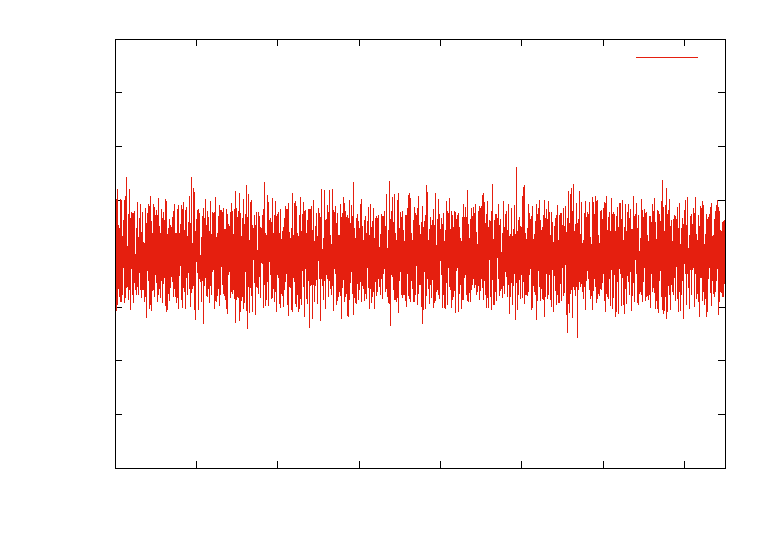
\includegraphics{plots/noise}}%
    \gplfronttext
  \end{picture}%
\endgroup

    \caption[]{average cero, root square -> flip it positive}
    \label{fig: noise}
\end{figure}

Figure \ref{fig: MonitorNoise138} shows the frequency domain noise. This means that the time domain is fourier transformed into the frequency domain. This method is one of the basic principles we use in this experiment to make research about the properties of the measured signals. The frequency domain noise shows very specific sharp peaks every \SI{50}{\hertz}. To be more specific the peaks in the middle of every hundred \si{\hertz} steps are way higher than those at \SI{1400}{\hertz}, \SI{1500}{\hertz} and so on. This results of the frequency in the power grid which is \SI{50}{\hertz} in Germany.
\textcolor{red}{wieso sind die geraden kleiner??? Steckdose erklärt eig nur peak bei 50hz und nicht die alle 50 hz}
Despite all sharp peaks there is also a slight increase of the amplitude around $\SI{1850 \pm 1000}{\frac{\mu \volt}{\hertz}}$ visible. This is explicable by the resonance frequency of instrument and its sensitvity around the lamorfrequency (\SI{1841.4}{\hertz} for water in Germany in July 2020). Nearby the lamorfrequency all our following measurements will be done that is why the instrument sensitvity is sharpend around this value.

\begin{figure}[H]
    \centering
    % GNUPLOT: LaTeX picture with Postscript
\begingroup
  % Encoding inside the plot.  In the header of your document, this encoding
  % should to defined, e.g., by using
  % \usepackage[cp1252,<other encodings>]{inputenc}
  \inputencoding{cp1252}%
  \makeatletter
  \providecommand\color[2][]{%
    \GenericError{(gnuplot) \space\space\space\@spaces}{%
      Package color not loaded in conjunction with
      terminal option `colourtext'%
    }{See the gnuplot documentation for explanation.%
    }{Either use 'blacktext' in gnuplot or load the package
      color.sty in LaTeX.}%
    \renewcommand\color[2][]{}%
  }%
  \providecommand\includegraphics[2][]{%
    \GenericError{(gnuplot) \space\space\space\@spaces}{%
      Package graphicx or graphics not loaded%
    }{See the gnuplot documentation for explanation.%
    }{The gnuplot epslatex terminal needs graphicx.sty or graphics.sty.}%
    \renewcommand\includegraphics[2][]{}%
  }%
  \providecommand\rotatebox[2]{#2}%
  \@ifundefined{ifGPcolor}{%
    \newif\ifGPcolor
    \GPcolorfalse
  }{}%
  \@ifundefined{ifGPblacktext}{%
    \newif\ifGPblacktext
    \GPblacktexttrue
  }{}%
  % define a \g@addto@macro without @ in the name:
  \let\gplgaddtomacro\g@addto@macro
  % define empty templates for all commands taking text:
  \gdef\gplbacktext{}%
  \gdef\gplfronttext{}%
  \makeatother
  \ifGPblacktext
    % no textcolor at all
    \def\colorrgb#1{}%
    \def\colorgray#1{}%
  \else
    % gray or color?
    \ifGPcolor
      \def\colorrgb#1{\color[rgb]{#1}}%
      \def\colorgray#1{\color[gray]{#1}}%
      \expandafter\def\csname LTw\endcsname{\color{white}}%
      \expandafter\def\csname LTb\endcsname{\color{black}}%
      \expandafter\def\csname LTa\endcsname{\color{black}}%
      \expandafter\def\csname LT0\endcsname{\color[rgb]{1,0,0}}%
      \expandafter\def\csname LT1\endcsname{\color[rgb]{0,1,0}}%
      \expandafter\def\csname LT2\endcsname{\color[rgb]{0,0,1}}%
      \expandafter\def\csname LT3\endcsname{\color[rgb]{1,0,1}}%
      \expandafter\def\csname LT4\endcsname{\color[rgb]{0,1,1}}%
      \expandafter\def\csname LT5\endcsname{\color[rgb]{1,1,0}}%
      \expandafter\def\csname LT6\endcsname{\color[rgb]{0,0,0}}%
      \expandafter\def\csname LT7\endcsname{\color[rgb]{1,0.3,0}}%
      \expandafter\def\csname LT8\endcsname{\color[rgb]{0.5,0.5,0.5}}%
    \else
      % gray
      \def\colorrgb#1{\color{black}}%
      \def\colorgray#1{\color[gray]{#1}}%
      \expandafter\def\csname LTw\endcsname{\color{white}}%
      \expandafter\def\csname LTb\endcsname{\color{black}}%
      \expandafter\def\csname LTa\endcsname{\color{black}}%
      \expandafter\def\csname LT0\endcsname{\color{black}}%
      \expandafter\def\csname LT1\endcsname{\color{black}}%
      \expandafter\def\csname LT2\endcsname{\color{black}}%
      \expandafter\def\csname LT3\endcsname{\color{black}}%
      \expandafter\def\csname LT4\endcsname{\color{black}}%
      \expandafter\def\csname LT5\endcsname{\color{black}}%
      \expandafter\def\csname LT6\endcsname{\color{black}}%
      \expandafter\def\csname LT7\endcsname{\color{black}}%
      \expandafter\def\csname LT8\endcsname{\color{black}}%
    \fi
  \fi
    \setlength{\unitlength}{0.0500bp}%
    \ifx\gptboxheight\undefined%
      \newlength{\gptboxheight}%
      \newlength{\gptboxwidth}%
      \newsavebox{\gptboxtext}%
    \fi%
    \setlength{\fboxrule}{0.5pt}%
    \setlength{\fboxsep}{1pt}%
\begin{picture}(7200.00,5040.00)%
    \gplgaddtomacro\gplbacktext{%
      \csname LTb\endcsname%%
      \put(682,704){\makebox(0,0)[r]{\strut{}$0$}}%
      \put(682,1390){\makebox(0,0)[r]{\strut{}$2$}}%
      \put(682,2076){\makebox(0,0)[r]{\strut{}$4$}}%
      \put(682,2762){\makebox(0,0)[r]{\strut{}$6$}}%
      \put(682,3447){\makebox(0,0)[r]{\strut{}$8$}}%
      \put(682,4133){\makebox(0,0)[r]{\strut{}$10$}}%
      \put(682,4819){\makebox(0,0)[r]{\strut{}$12$}}%
      \put(814,484){\makebox(0,0){\strut{}$1400$}}%
      \put(1479,484){\makebox(0,0){\strut{}$1500$}}%
      \put(2145,484){\makebox(0,0){\strut{}$1600$}}%
      \put(2810,484){\makebox(0,0){\strut{}$1700$}}%
      \put(3476,484){\makebox(0,0){\strut{}$1800$}}%
      \put(4141,484){\makebox(0,0){\strut{}$1900$}}%
      \put(4807,484){\makebox(0,0){\strut{}$2000$}}%
      \put(5472,484){\makebox(0,0){\strut{}$2100$}}%
      \put(6138,484){\makebox(0,0){\strut{}$2200$}}%
      \put(6803,484){\makebox(0,0){\strut{}$2300$}}%
    }%
    \gplgaddtomacro\gplfronttext{%
      \csname LTb\endcsname%%
      \put(308,2761){\rotatebox{-270}{\makebox(0,0){\strut{}Amplitude in $\si{\frac{\mu \volt}{\hertz}}$}}}%
      \put(3808,154){\makebox(0,0){\strut{}Frequency in $\si{\hertz}$}}%
      \csname LTb\endcsname%%
      \put(5816,4646){\makebox(0,0)[r]{\strut{}noise magnitude spectrum}}%
    }%
    \gplbacktext
    \put(0,0){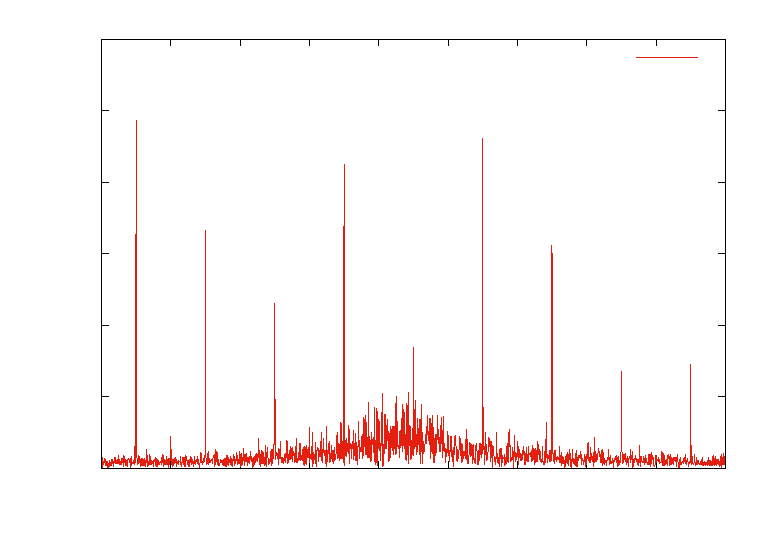
\includegraphics{plots/MonitorNoise138}}%
    \gplfronttext
  \end{picture}%
\endgroup

    \caption[]{}
    \label{fig: MonitorNoise138}
\end{figure}


% !TEX root = main.tex
\section{Coil Analysis}
\label{sec:CoilAnalyssis}
Now knowing that we have a acceptable noise value under \SI{10}{\mu \volt}, we can analyse the coil. In order to do so we explain the general approach of NMR signals first. To measure a NMR signal a pulse and collect measurement has to be done. Therefore the B$_1$ coil (transmit and collect coil) has to apply a pulse. This pulse changes the spins direction out of its thermal equilibrium (along z-axes, due to the earths magnetic field B$_e$) into a direction with a component in the transversal plain. Therefore the B$_1$ coil collects a signal, because its aligned orthogonal to B$_e$. The transmit and collect procedure is based on Faraday's law of induction. Figure \ref{fig: PulsandcollectValesignal} exemplary shows such a collect signal by the B$_1$ coil. Every following measurement in this paper is based on the procedure of pulse and collect.

\begin{figure}[H]
    \centering
    % GNUPLOT: LaTeX picture with Postscript
\begingroup
  % Encoding inside the plot.  In the header of your document, this encoding
  % should to defined, e.g., by using
  % \usepackage[cp1252,<other encodings>]{inputenc}
  \inputencoding{cp1252}%
  \makeatletter
  \providecommand\color[2][]{%
    \GenericError{(gnuplot) \space\space\space\@spaces}{%
      Package color not loaded in conjunction with
      terminal option `colourtext'%
    }{See the gnuplot documentation for explanation.%
    }{Either use 'blacktext' in gnuplot or load the package
      color.sty in LaTeX.}%
    \renewcommand\color[2][]{}%
  }%
  \providecommand\includegraphics[2][]{%
    \GenericError{(gnuplot) \space\space\space\@spaces}{%
      Package graphicx or graphics not loaded%
    }{See the gnuplot documentation for explanation.%
    }{The gnuplot epslatex terminal needs graphicx.sty or graphics.sty.}%
    \renewcommand\includegraphics[2][]{}%
  }%
  \providecommand\rotatebox[2]{#2}%
  \@ifundefined{ifGPcolor}{%
    \newif\ifGPcolor
    \GPcolorfalse
  }{}%
  \@ifundefined{ifGPblacktext}{%
    \newif\ifGPblacktext
    \GPblacktexttrue
  }{}%
  % define a \g@addto@macro without @ in the name:
  \let\gplgaddtomacro\g@addto@macro
  % define empty templates for all commands taking text:
  \gdef\gplbacktext{}%
  \gdef\gplfronttext{}%
  \makeatother
  \ifGPblacktext
    % no textcolor at all
    \def\colorrgb#1{}%
    \def\colorgray#1{}%
  \else
    % gray or color?
    \ifGPcolor
      \def\colorrgb#1{\color[rgb]{#1}}%
      \def\colorgray#1{\color[gray]{#1}}%
      \expandafter\def\csname LTw\endcsname{\color{white}}%
      \expandafter\def\csname LTb\endcsname{\color{black}}%
      \expandafter\def\csname LTa\endcsname{\color{black}}%
      \expandafter\def\csname LT0\endcsname{\color[rgb]{1,0,0}}%
      \expandafter\def\csname LT1\endcsname{\color[rgb]{0,1,0}}%
      \expandafter\def\csname LT2\endcsname{\color[rgb]{0,0,1}}%
      \expandafter\def\csname LT3\endcsname{\color[rgb]{1,0,1}}%
      \expandafter\def\csname LT4\endcsname{\color[rgb]{0,1,1}}%
      \expandafter\def\csname LT5\endcsname{\color[rgb]{1,1,0}}%
      \expandafter\def\csname LT6\endcsname{\color[rgb]{0,0,0}}%
      \expandafter\def\csname LT7\endcsname{\color[rgb]{1,0.3,0}}%
      \expandafter\def\csname LT8\endcsname{\color[rgb]{0.5,0.5,0.5}}%
    \else
      % gray
      \def\colorrgb#1{\color{black}}%
      \def\colorgray#1{\color[gray]{#1}}%
      \expandafter\def\csname LTw\endcsname{\color{white}}%
      \expandafter\def\csname LTb\endcsname{\color{black}}%
      \expandafter\def\csname LTa\endcsname{\color{black}}%
      \expandafter\def\csname LT0\endcsname{\color{black}}%
      \expandafter\def\csname LT1\endcsname{\color{black}}%
      \expandafter\def\csname LT2\endcsname{\color{black}}%
      \expandafter\def\csname LT3\endcsname{\color{black}}%
      \expandafter\def\csname LT4\endcsname{\color{black}}%
      \expandafter\def\csname LT5\endcsname{\color{black}}%
      \expandafter\def\csname LT6\endcsname{\color{black}}%
      \expandafter\def\csname LT7\endcsname{\color{black}}%
      \expandafter\def\csname LT8\endcsname{\color{black}}%
    \fi
  \fi
    \setlength{\unitlength}{0.0500bp}%
    \ifx\gptboxheight\undefined%
      \newlength{\gptboxheight}%
      \newlength{\gptboxwidth}%
      \newsavebox{\gptboxtext}%
    \fi%
    \setlength{\fboxrule}{0.5pt}%
    \setlength{\fboxsep}{1pt}%
\begin{picture}(7200.00,5040.00)%
    \gplgaddtomacro\gplbacktext{%
      \csname LTb\endcsname%%
      \put(814,704){\makebox(0,0)[r]{\strut{}$-80$}}%
      \put(814,1218){\makebox(0,0)[r]{\strut{}$-60$}}%
      \put(814,1733){\makebox(0,0)[r]{\strut{}$-40$}}%
      \put(814,2247){\makebox(0,0)[r]{\strut{}$-20$}}%
      \put(814,2762){\makebox(0,0)[r]{\strut{}$0$}}%
      \put(814,3276){\makebox(0,0)[r]{\strut{}$20$}}%
      \put(814,3790){\makebox(0,0)[r]{\strut{}$40$}}%
      \put(814,4305){\makebox(0,0)[r]{\strut{}$60$}}%
      \put(814,4819){\makebox(0,0)[r]{\strut{}$80$}}%
      \put(946,484){\makebox(0,0){\strut{}$0$}}%
      \put(1727,484){\makebox(0,0){\strut{}$0.2$}}%
      \put(2508,484){\makebox(0,0){\strut{}$0.4$}}%
      \put(3289,484){\makebox(0,0){\strut{}$0.6$}}%
      \put(4070,484){\makebox(0,0){\strut{}$0.8$}}%
      \put(4851,484){\makebox(0,0){\strut{}$1$}}%
      \put(5632,484){\makebox(0,0){\strut{}$1.2$}}%
      \put(6413,484){\makebox(0,0){\strut{}$1.4$}}%
    }%
    \gplgaddtomacro\gplfronttext{%
      \csname LTb\endcsname%%
      \put(209,2761){\rotatebox{-270}{\makebox(0,0){\strut{}Amplitude in $\si{\mu \volt}$}}}%
      \put(3874,154){\makebox(0,0){\strut{}Time in $\si{\second}$}}%
      \csname LTb\endcsname%%
      \put(5816,4646){\makebox(0,0)[r]{\strut{}FID data}}%
    }%
    \gplbacktext
    \put(0,0){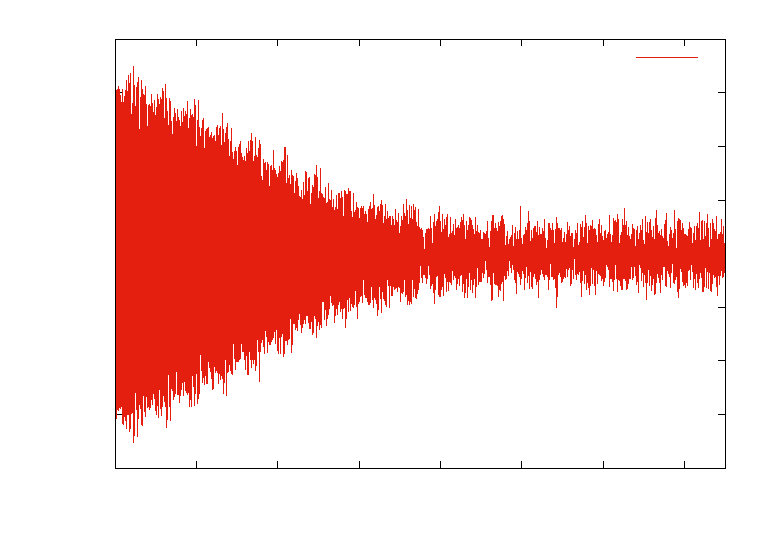
\includegraphics{plots/PulsandcollectValesignal}}%
    \gplfronttext
  \end{picture}%
\endgroup

    \caption[Example signal for a pulse and collect signal made by the B$_1$ coil.]{Example signal for a pulse and collect signal made by the B$_1$ coil. The example signal is taken from a FID signal.}
    \label{fig: PulsandcollectValesignal}
\end{figure}

Due to the fact that the B$_1$ coil is a tuned LCR circuit a resonance frequency exists, which can be caluclated by following formula:
\begin{align}
    \omega_{calc} = \frac{1}{\sqrt{L \cdot C}} \ .
    \label{eq: lamorcalc}
\end{align}
To analyse the B$_1$ coil the resonance frequency versus the capacity is measured. Therefore the B$_1$ coil transmits a signal. Due to this signal the response of the coil can be measured. This signal is than fourie tranformed and the resonance frequency can be deduced from the frequency domain (maxmimum in the frequency domain). This procedure is repeated automatically by the computer programm ''\textit{Prospa}'' for different capacities. By changing the capacity we can examen the best capacity in dependence of the lamor frequency. Figure \ref{fig: Coilanalyse} shows the measured and theoretically calculated resonance frequency (Equation \ref{eq: lamorcalc}; $L = \SI{0.417}{\henry}$) in dependence of the capacity. The horizontal line represents the lamor frequency of \SI{1841.4}{\hertz} for water in Germany in July 2020. To gain this value the vertical component of the earths magnetic field ( \SI{43248.8}{\nano \tesla}\textcolor{red}{Quelle Marc}) is multiplied to the gyromagnetic ration $\SI{42.577}{\frac{\mega \hertz}{\tesla}}$. \textcolor{red}{Quelle Marc}. The vertical line represents the correct capacity we should use for our measurement, due to the resonance frequency of the lamor frequency. In this case the correct capacity is \SI{13.8}{\nano \farad}. For the calculated resonance frequency the correct capacity would be \SI{17.9}{\nano \farad}. It is not deniable that the measured curve is not parallel to the measured resonance frequency. This probably has its cause in the not fix inductance $L$. Due to heating of the coil $L$ might change a little by increasing capacity and thus the calculated curve does not fit to the measured one.


\begin{figure}[H]
    \centering
    % GNUPLOT: LaTeX picture with Postscript
\begingroup
  % Encoding inside the plot.  In the header of your document, this encoding
  % should to defined, e.g., by using
  % \usepackage[cp1252,<other encodings>]{inputenc}
  \inputencoding{cp1252}%
  \makeatletter
  \providecommand\color[2][]{%
    \GenericError{(gnuplot) \space\space\space\@spaces}{%
      Package color not loaded in conjunction with
      terminal option `colourtext'%
    }{See the gnuplot documentation for explanation.%
    }{Either use 'blacktext' in gnuplot or load the package
      color.sty in LaTeX.}%
    \renewcommand\color[2][]{}%
  }%
  \providecommand\includegraphics[2][]{%
    \GenericError{(gnuplot) \space\space\space\@spaces}{%
      Package graphicx or graphics not loaded%
    }{See the gnuplot documentation for explanation.%
    }{The gnuplot epslatex terminal needs graphicx.sty or graphics.sty.}%
    \renewcommand\includegraphics[2][]{}%
  }%
  \providecommand\rotatebox[2]{#2}%
  \@ifundefined{ifGPcolor}{%
    \newif\ifGPcolor
    \GPcolorfalse
  }{}%
  \@ifundefined{ifGPblacktext}{%
    \newif\ifGPblacktext
    \GPblacktexttrue
  }{}%
  % define a \g@addto@macro without @ in the name:
  \let\gplgaddtomacro\g@addto@macro
  % define empty templates for all commands taking text:
  \gdef\gplbacktext{}%
  \gdef\gplfronttext{}%
  \makeatother
  \ifGPblacktext
    % no textcolor at all
    \def\colorrgb#1{}%
    \def\colorgray#1{}%
  \else
    % gray or color?
    \ifGPcolor
      \def\colorrgb#1{\color[rgb]{#1}}%
      \def\colorgray#1{\color[gray]{#1}}%
      \expandafter\def\csname LTw\endcsname{\color{white}}%
      \expandafter\def\csname LTb\endcsname{\color{black}}%
      \expandafter\def\csname LTa\endcsname{\color{black}}%
      \expandafter\def\csname LT0\endcsname{\color[rgb]{1,0,0}}%
      \expandafter\def\csname LT1\endcsname{\color[rgb]{0,1,0}}%
      \expandafter\def\csname LT2\endcsname{\color[rgb]{0,0,1}}%
      \expandafter\def\csname LT3\endcsname{\color[rgb]{1,0,1}}%
      \expandafter\def\csname LT4\endcsname{\color[rgb]{0,1,1}}%
      \expandafter\def\csname LT5\endcsname{\color[rgb]{1,1,0}}%
      \expandafter\def\csname LT6\endcsname{\color[rgb]{0,0,0}}%
      \expandafter\def\csname LT7\endcsname{\color[rgb]{1,0.3,0}}%
      \expandafter\def\csname LT8\endcsname{\color[rgb]{0.5,0.5,0.5}}%
    \else
      % gray
      \def\colorrgb#1{\color{black}}%
      \def\colorgray#1{\color[gray]{#1}}%
      \expandafter\def\csname LTw\endcsname{\color{white}}%
      \expandafter\def\csname LTb\endcsname{\color{black}}%
      \expandafter\def\csname LTa\endcsname{\color{black}}%
      \expandafter\def\csname LT0\endcsname{\color{black}}%
      \expandafter\def\csname LT1\endcsname{\color{black}}%
      \expandafter\def\csname LT2\endcsname{\color{black}}%
      \expandafter\def\csname LT3\endcsname{\color{black}}%
      \expandafter\def\csname LT4\endcsname{\color{black}}%
      \expandafter\def\csname LT5\endcsname{\color{black}}%
      \expandafter\def\csname LT6\endcsname{\color{black}}%
      \expandafter\def\csname LT7\endcsname{\color{black}}%
      \expandafter\def\csname LT8\endcsname{\color{black}}%
    \fi
  \fi
    \setlength{\unitlength}{0.0500bp}%
    \ifx\gptboxheight\undefined%
      \newlength{\gptboxheight}%
      \newlength{\gptboxwidth}%
      \newsavebox{\gptboxtext}%
    \fi%
    \setlength{\fboxrule}{0.5pt}%
    \setlength{\fboxsep}{1pt}%
\begin{picture}(7200.00,5040.00)%
    \gplgaddtomacro\gplbacktext{%
      \csname LTb\endcsname%%
      \put(946,704){\makebox(0,0)[r]{\strut{}$1500$}}%
      \put(946,1527){\makebox(0,0)[r]{\strut{}$2000$}}%
      \put(946,2350){\makebox(0,0)[r]{\strut{}$2500$}}%
      \put(946,3173){\makebox(0,0)[r]{\strut{}$3000$}}%
      \put(946,3996){\makebox(0,0)[r]{\strut{}$3500$}}%
      \put(946,4819){\makebox(0,0)[r]{\strut{}$4000$}}%
      \put(1794,484){\makebox(0,0){\strut{}$6$}}%
      \put(2688,484){\makebox(0,0){\strut{}$8$}}%
      \put(3583,484){\makebox(0,0){\strut{}$10$}}%
      \put(4477,484){\makebox(0,0){\strut{}$12$}}%
      \put(5372,484){\makebox(0,0){\strut{}$14$}}%
      \put(6266,484){\makebox(0,0){\strut{}$16$}}%
    }%
    \gplgaddtomacro\gplfronttext{%
      \csname LTb\endcsname%%
      \put(209,2761){\rotatebox{-270}{\makebox(0,0){\strut{}Frequency $\si{\hertz}$}}}%
      \put(3940,154){\makebox(0,0){\strut{}Capacity in $\si{\nano \farad}$}}%
      \csname LTb\endcsname%%
      \put(5816,4646){\makebox(0,0)[r]{\strut{}measured resonance frequency}}%
      \csname LTb\endcsname%%
      \put(5816,4426){\makebox(0,0)[r]{\strut{}calculated resonance frequency}}%
    }%
    \gplbacktext
    \put(0,0){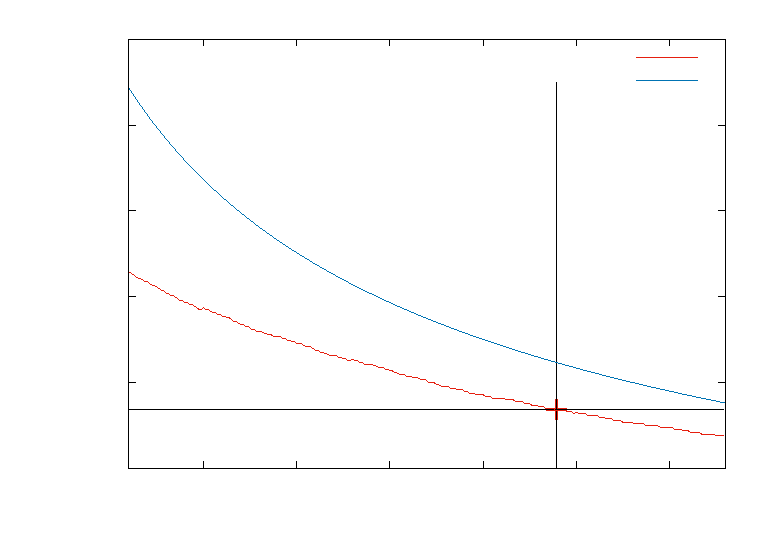
\includegraphics{plots/Coilanalyse}}%
    \gplfronttext
  \end{picture}%
\endgroup

    \caption[This figure shows the measured and calculated resonance frequencies for different capacities.]{This figure shows the measured and calculated resonance frequencies for different capacities. The marked cross represents the lamor frequency of \SI{1841.4}{\hertz} for water in Germany in July 2020.}
    \label{fig: Coilanalyse}
\end{figure}
% !TEX root = main.tex
\section{Optimization and Characterisation of FID in water sample}
\label{sec:OptimizationandCharacterisationofFIDinwatersample}

\textcolor{red}{insert previous values}

ask: is it ok to explain what autoshim does and don´t plot any graphs at all? We don´t have data for an example plot -> yes

\begin{figure}[H]
    \centering
    % GNUPLOT: LaTeX picture with Postscript
\begingroup
  % Encoding inside the plot.  In the header of your document, this encoding
  % should to defined, e.g., by using
  % \usepackage[cp1252,<other encodings>]{inputenc}
  \inputencoding{cp1252}%
  \makeatletter
  \providecommand\color[2][]{%
    \GenericError{(gnuplot) \space\space\space\@spaces}{%
      Package color not loaded in conjunction with
      terminal option `colourtext'%
    }{See the gnuplot documentation for explanation.%
    }{Either use 'blacktext' in gnuplot or load the package
      color.sty in LaTeX.}%
    \renewcommand\color[2][]{}%
  }%
  \providecommand\includegraphics[2][]{%
    \GenericError{(gnuplot) \space\space\space\@spaces}{%
      Package graphicx or graphics not loaded%
    }{See the gnuplot documentation for explanation.%
    }{The gnuplot epslatex terminal needs graphicx.sty or graphics.sty.}%
    \renewcommand\includegraphics[2][]{}%
  }%
  \providecommand\rotatebox[2]{#2}%
  \@ifundefined{ifGPcolor}{%
    \newif\ifGPcolor
    \GPcolorfalse
  }{}%
  \@ifundefined{ifGPblacktext}{%
    \newif\ifGPblacktext
    \GPblacktexttrue
  }{}%
  % define a \g@addto@macro without @ in the name:
  \let\gplgaddtomacro\g@addto@macro
  % define empty templates for all commands taking text:
  \gdef\gplbacktext{}%
  \gdef\gplfronttext{}%
  \makeatother
  \ifGPblacktext
    % no textcolor at all
    \def\colorrgb#1{}%
    \def\colorgray#1{}%
  \else
    % gray or color?
    \ifGPcolor
      \def\colorrgb#1{\color[rgb]{#1}}%
      \def\colorgray#1{\color[gray]{#1}}%
      \expandafter\def\csname LTw\endcsname{\color{white}}%
      \expandafter\def\csname LTb\endcsname{\color{black}}%
      \expandafter\def\csname LTa\endcsname{\color{black}}%
      \expandafter\def\csname LT0\endcsname{\color[rgb]{1,0,0}}%
      \expandafter\def\csname LT1\endcsname{\color[rgb]{0,1,0}}%
      \expandafter\def\csname LT2\endcsname{\color[rgb]{0,0,1}}%
      \expandafter\def\csname LT3\endcsname{\color[rgb]{1,0,1}}%
      \expandafter\def\csname LT4\endcsname{\color[rgb]{0,1,1}}%
      \expandafter\def\csname LT5\endcsname{\color[rgb]{1,1,0}}%
      \expandafter\def\csname LT6\endcsname{\color[rgb]{0,0,0}}%
      \expandafter\def\csname LT7\endcsname{\color[rgb]{1,0.3,0}}%
      \expandafter\def\csname LT8\endcsname{\color[rgb]{0.5,0.5,0.5}}%
    \else
      % gray
      \def\colorrgb#1{\color{black}}%
      \def\colorgray#1{\color[gray]{#1}}%
      \expandafter\def\csname LTw\endcsname{\color{white}}%
      \expandafter\def\csname LTb\endcsname{\color{black}}%
      \expandafter\def\csname LTa\endcsname{\color{black}}%
      \expandafter\def\csname LT0\endcsname{\color{black}}%
      \expandafter\def\csname LT1\endcsname{\color{black}}%
      \expandafter\def\csname LT2\endcsname{\color{black}}%
      \expandafter\def\csname LT3\endcsname{\color{black}}%
      \expandafter\def\csname LT4\endcsname{\color{black}}%
      \expandafter\def\csname LT5\endcsname{\color{black}}%
      \expandafter\def\csname LT6\endcsname{\color{black}}%
      \expandafter\def\csname LT7\endcsname{\color{black}}%
      \expandafter\def\csname LT8\endcsname{\color{black}}%
    \fi
  \fi
    \setlength{\unitlength}{0.0500bp}%
    \ifx\gptboxheight\undefined%
      \newlength{\gptboxheight}%
      \newlength{\gptboxwidth}%
      \newsavebox{\gptboxtext}%
    \fi%
    \setlength{\fboxrule}{0.5pt}%
    \setlength{\fboxsep}{1pt}%
\begin{picture}(7200.00,5040.00)%
    \gplgaddtomacro\gplbacktext{%
      \csname LTb\endcsname%%
      \put(814,704){\makebox(0,0)[r]{\strut{}$60$}}%
      \put(814,1527){\makebox(0,0)[r]{\strut{}$80$}}%
      \put(814,2350){\makebox(0,0)[r]{\strut{}$100$}}%
      \put(814,3173){\makebox(0,0)[r]{\strut{}$120$}}%
      \put(814,3996){\makebox(0,0)[r]{\strut{}$140$}}%
      \put(814,4819){\makebox(0,0)[r]{\strut{}$160$}}%
      \put(946,484){\makebox(0,0){\strut{}$0$}}%
      \put(1678,484){\makebox(0,0){\strut{}$0.5$}}%
      \put(2410,484){\makebox(0,0){\strut{}$1$}}%
      \put(3142,484){\makebox(0,0){\strut{}$1.5$}}%
      \put(3875,484){\makebox(0,0){\strut{}$2$}}%
      \put(4607,484){\makebox(0,0){\strut{}$2.5$}}%
      \put(5339,484){\makebox(0,0){\strut{}$3$}}%
      \put(6071,484){\makebox(0,0){\strut{}$3.5$}}%
      \put(6803,484){\makebox(0,0){\strut{}$4$}}%
    }%
    \gplgaddtomacro\gplfronttext{%
      \csname LTb\endcsname%%
      \put(209,2761){\rotatebox{-270}{\makebox(0,0){\strut{}FID amplitude}}}%
      \put(3874,154){\makebox(0,0){\strut{}$B_1$ pulse in $\si{}{ms}$}}%
      \csname LTb\endcsname%%
      \put(5816,4646){\makebox(0,0)[r]{\strut{}measured resonance amplitude}}%
    }%
    \gplbacktext
    \put(0,0){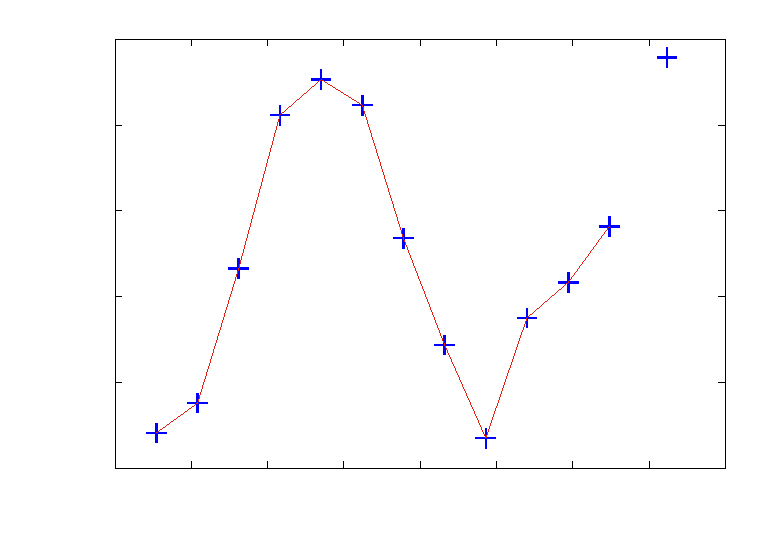
\includegraphics{plots/B1dauer}}%
    \gplfronttext
  \end{picture}%
\endgroup

    \caption[]{ask: periodicity due to duration of B$_1$, \SI{0}{\degree} -> \SI{90}{\degree} -> \SI{180}{\degree} -> \SI{270}{\degree}? -> yes}
    \label{fig:B1dauer}
\end{figure}

\begin{figure}[H]
    \centering
    % GNUPLOT: LaTeX picture with Postscript
\begingroup
  % Encoding inside the plot.  In the header of your document, this encoding
  % should to defined, e.g., by using
  % \usepackage[cp1252,<other encodings>]{inputenc}
  \inputencoding{cp1252}%
  \makeatletter
  \providecommand\color[2][]{%
    \GenericError{(gnuplot) \space\space\space\@spaces}{%
      Package color not loaded in conjunction with
      terminal option `colourtext'%
    }{See the gnuplot documentation for explanation.%
    }{Either use 'blacktext' in gnuplot or load the package
      color.sty in LaTeX.}%
    \renewcommand\color[2][]{}%
  }%
  \providecommand\includegraphics[2][]{%
    \GenericError{(gnuplot) \space\space\space\@spaces}{%
      Package graphicx or graphics not loaded%
    }{See the gnuplot documentation for explanation.%
    }{The gnuplot epslatex terminal needs graphicx.sty or graphics.sty.}%
    \renewcommand\includegraphics[2][]{}%
  }%
  \providecommand\rotatebox[2]{#2}%
  \@ifundefined{ifGPcolor}{%
    \newif\ifGPcolor
    \GPcolorfalse
  }{}%
  \@ifundefined{ifGPblacktext}{%
    \newif\ifGPblacktext
    \GPblacktexttrue
  }{}%
  % define a \g@addto@macro without @ in the name:
  \let\gplgaddtomacro\g@addto@macro
  % define empty templates for all commands taking text:
  \gdef\gplbacktext{}%
  \gdef\gplfronttext{}%
  \makeatother
  \ifGPblacktext
    % no textcolor at all
    \def\colorrgb#1{}%
    \def\colorgray#1{}%
  \else
    % gray or color?
    \ifGPcolor
      \def\colorrgb#1{\color[rgb]{#1}}%
      \def\colorgray#1{\color[gray]{#1}}%
      \expandafter\def\csname LTw\endcsname{\color{white}}%
      \expandafter\def\csname LTb\endcsname{\color{black}}%
      \expandafter\def\csname LTa\endcsname{\color{black}}%
      \expandafter\def\csname LT0\endcsname{\color[rgb]{1,0,0}}%
      \expandafter\def\csname LT1\endcsname{\color[rgb]{0,1,0}}%
      \expandafter\def\csname LT2\endcsname{\color[rgb]{0,0,1}}%
      \expandafter\def\csname LT3\endcsname{\color[rgb]{1,0,1}}%
      \expandafter\def\csname LT4\endcsname{\color[rgb]{0,1,1}}%
      \expandafter\def\csname LT5\endcsname{\color[rgb]{1,1,0}}%
      \expandafter\def\csname LT6\endcsname{\color[rgb]{0,0,0}}%
      \expandafter\def\csname LT7\endcsname{\color[rgb]{1,0.3,0}}%
      \expandafter\def\csname LT8\endcsname{\color[rgb]{0.5,0.5,0.5}}%
    \else
      % gray
      \def\colorrgb#1{\color{black}}%
      \def\colorgray#1{\color[gray]{#1}}%
      \expandafter\def\csname LTw\endcsname{\color{white}}%
      \expandafter\def\csname LTb\endcsname{\color{black}}%
      \expandafter\def\csname LTa\endcsname{\color{black}}%
      \expandafter\def\csname LT0\endcsname{\color{black}}%
      \expandafter\def\csname LT1\endcsname{\color{black}}%
      \expandafter\def\csname LT2\endcsname{\color{black}}%
      \expandafter\def\csname LT3\endcsname{\color{black}}%
      \expandafter\def\csname LT4\endcsname{\color{black}}%
      \expandafter\def\csname LT5\endcsname{\color{black}}%
      \expandafter\def\csname LT6\endcsname{\color{black}}%
      \expandafter\def\csname LT7\endcsname{\color{black}}%
      \expandafter\def\csname LT8\endcsname{\color{black}}%
    \fi
  \fi
    \setlength{\unitlength}{0.0500bp}%
    \ifx\gptboxheight\undefined%
      \newlength{\gptboxheight}%
      \newlength{\gptboxwidth}%
      \newsavebox{\gptboxtext}%
    \fi%
    \setlength{\fboxrule}{0.5pt}%
    \setlength{\fboxsep}{1pt}%
\begin{picture}(7200.00,5040.00)%
    \gplgaddtomacro\gplbacktext{%
      \csname LTb\endcsname%%
      \put(682,704){\makebox(0,0)[r]{\strut{}$0$}}%
      \put(682,1161){\makebox(0,0)[r]{\strut{}$10$}}%
      \put(682,1618){\makebox(0,0)[r]{\strut{}$20$}}%
      \put(682,2076){\makebox(0,0)[r]{\strut{}$30$}}%
      \put(682,2533){\makebox(0,0)[r]{\strut{}$40$}}%
      \put(682,2990){\makebox(0,0)[r]{\strut{}$50$}}%
      \put(682,3447){\makebox(0,0)[r]{\strut{}$60$}}%
      \put(682,3905){\makebox(0,0)[r]{\strut{}$70$}}%
      \put(682,4362){\makebox(0,0)[r]{\strut{}$80$}}%
      \put(682,4819){\makebox(0,0)[r]{\strut{}$90$}}%
      \put(814,484){\makebox(0,0){\strut{}$1800$}}%
      \put(2012,484){\makebox(0,0){\strut{}$1820$}}%
      \put(3210,484){\makebox(0,0){\strut{}$1840$}}%
      \put(4407,484){\makebox(0,0){\strut{}$1860$}}%
      \put(5605,484){\makebox(0,0){\strut{}$1880$}}%
      \put(6803,484){\makebox(0,0){\strut{}$1900$}}%
    }%
    \gplgaddtomacro\gplfronttext{%
      \csname LTb\endcsname%%
      \put(209,2761){\rotatebox{-270}{\makebox(0,0){\strut{}Amplitude in $\si{\mu \volt}$}}}%
      \put(3808,154){\makebox(0,0){\strut{}Frequency in $\si{\hertz}$}}%
      \csname LTb\endcsname%%
      \put(5816,4646){\makebox(0,0)[r]{\strut{}$\SI{0.27}{\milli \second}$ B$_1$ duration}}%
      \csname LTb\endcsname%%
      \put(5816,4426){\makebox(0,0)[r]{\strut{}$\SI{1.35}{\milli \second}$ B$_1$ duration}}%
    }%
    \gplbacktext
    \put(0,0){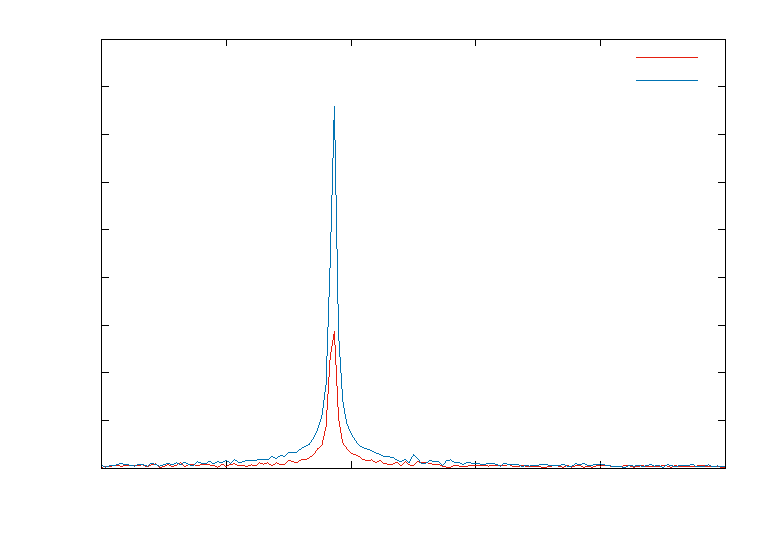
\includegraphics{plots/138_puls_and_collect_number_of_delay25ms_Pulseduration0_27ms}}%
    \gplfronttext
  \end{picture}%
\endgroup

    \caption[]{}
    \label{fig:pulsedurationbeispiel}
\end{figure}

\begin{figure}[H]
    \centering
    % GNUPLOT: LaTeX picture with Postscript
\begingroup
  % Encoding inside the plot.  In the header of your document, this encoding
  % should to defined, e.g., by using
  % \usepackage[cp1252,<other encodings>]{inputenc}
  \inputencoding{cp1252}%
  \makeatletter
  \providecommand\color[2][]{%
    \GenericError{(gnuplot) \space\space\space\@spaces}{%
      Package color not loaded in conjunction with
      terminal option `colourtext'%
    }{See the gnuplot documentation for explanation.%
    }{Either use 'blacktext' in gnuplot or load the package
      color.sty in LaTeX.}%
    \renewcommand\color[2][]{}%
  }%
  \providecommand\includegraphics[2][]{%
    \GenericError{(gnuplot) \space\space\space\@spaces}{%
      Package graphicx or graphics not loaded%
    }{See the gnuplot documentation for explanation.%
    }{The gnuplot epslatex terminal needs graphicx.sty or graphics.sty.}%
    \renewcommand\includegraphics[2][]{}%
  }%
  \providecommand\rotatebox[2]{#2}%
  \@ifundefined{ifGPcolor}{%
    \newif\ifGPcolor
    \GPcolorfalse
  }{}%
  \@ifundefined{ifGPblacktext}{%
    \newif\ifGPblacktext
    \GPblacktexttrue
  }{}%
  % define a \g@addto@macro without @ in the name:
  \let\gplgaddtomacro\g@addto@macro
  % define empty templates for all commands taking text:
  \gdef\gplbacktext{}%
  \gdef\gplfronttext{}%
  \makeatother
  \ifGPblacktext
    % no textcolor at all
    \def\colorrgb#1{}%
    \def\colorgray#1{}%
  \else
    % gray or color?
    \ifGPcolor
      \def\colorrgb#1{\color[rgb]{#1}}%
      \def\colorgray#1{\color[gray]{#1}}%
      \expandafter\def\csname LTw\endcsname{\color{white}}%
      \expandafter\def\csname LTb\endcsname{\color{black}}%
      \expandafter\def\csname LTa\endcsname{\color{black}}%
      \expandafter\def\csname LT0\endcsname{\color[rgb]{1,0,0}}%
      \expandafter\def\csname LT1\endcsname{\color[rgb]{0,1,0}}%
      \expandafter\def\csname LT2\endcsname{\color[rgb]{0,0,1}}%
      \expandafter\def\csname LT3\endcsname{\color[rgb]{1,0,1}}%
      \expandafter\def\csname LT4\endcsname{\color[rgb]{0,1,1}}%
      \expandafter\def\csname LT5\endcsname{\color[rgb]{1,1,0}}%
      \expandafter\def\csname LT6\endcsname{\color[rgb]{0,0,0}}%
      \expandafter\def\csname LT7\endcsname{\color[rgb]{1,0.3,0}}%
      \expandafter\def\csname LT8\endcsname{\color[rgb]{0.5,0.5,0.5}}%
    \else
      % gray
      \def\colorrgb#1{\color{black}}%
      \def\colorgray#1{\color[gray]{#1}}%
      \expandafter\def\csname LTw\endcsname{\color{white}}%
      \expandafter\def\csname LTb\endcsname{\color{black}}%
      \expandafter\def\csname LTa\endcsname{\color{black}}%
      \expandafter\def\csname LT0\endcsname{\color{black}}%
      \expandafter\def\csname LT1\endcsname{\color{black}}%
      \expandafter\def\csname LT2\endcsname{\color{black}}%
      \expandafter\def\csname LT3\endcsname{\color{black}}%
      \expandafter\def\csname LT4\endcsname{\color{black}}%
      \expandafter\def\csname LT5\endcsname{\color{black}}%
      \expandafter\def\csname LT6\endcsname{\color{black}}%
      \expandafter\def\csname LT7\endcsname{\color{black}}%
      \expandafter\def\csname LT8\endcsname{\color{black}}%
    \fi
  \fi
    \setlength{\unitlength}{0.0500bp}%
    \ifx\gptboxheight\undefined%
      \newlength{\gptboxheight}%
      \newlength{\gptboxwidth}%
      \newsavebox{\gptboxtext}%
    \fi%
    \setlength{\fboxrule}{0.5pt}%
    \setlength{\fboxsep}{1pt}%
\begin{picture}(7200.00,5040.00)%
    \gplgaddtomacro\gplbacktext{%
      \csname LTb\endcsname%%
      \put(814,704){\makebox(0,0)[r]{\strut{}$0$}}%
      \put(814,1390){\makebox(0,0)[r]{\strut{}$20$}}%
      \put(814,2076){\makebox(0,0)[r]{\strut{}$40$}}%
      \put(814,2762){\makebox(0,0)[r]{\strut{}$60$}}%
      \put(814,3447){\makebox(0,0)[r]{\strut{}$80$}}%
      \put(814,4133){\makebox(0,0)[r]{\strut{}$100$}}%
      \put(814,4819){\makebox(0,0)[r]{\strut{}$120$}}%
      \put(946,484){\makebox(0,0){\strut{}$1650$}}%
      \put(1678,484){\makebox(0,0){\strut{}$1700$}}%
      \put(2410,484){\makebox(0,0){\strut{}$1750$}}%
      \put(3142,484){\makebox(0,0){\strut{}$1800$}}%
      \put(3875,484){\makebox(0,0){\strut{}$1850$}}%
      \put(4607,484){\makebox(0,0){\strut{}$1900$}}%
      \put(5339,484){\makebox(0,0){\strut{}$1950$}}%
      \put(6071,484){\makebox(0,0){\strut{}$2000$}}%
      \put(6803,484){\makebox(0,0){\strut{}$2050$}}%
    }%
    \gplgaddtomacro\gplfronttext{%
      \csname LTb\endcsname%%
      \put(209,2761){\rotatebox{-270}{\makebox(0,0){\strut{}Amplitude}}}%
      \put(3874,154){\makebox(0,0){\strut{}Frequency in $\si{\hertz}$}}%
      \csname LTb\endcsname%%
      \put(5816,4646){\makebox(0,0)[r]{\strut{}capacity $\SI{13.8}{\nano \farad}$}}%
      \csname LTb\endcsname%%
      \put(5816,4426){\makebox(0,0)[r]{\strut{}capacity $\SI{14.2}{\nano \farad}$}}%
    }%
    \gplbacktext
    \put(0,0){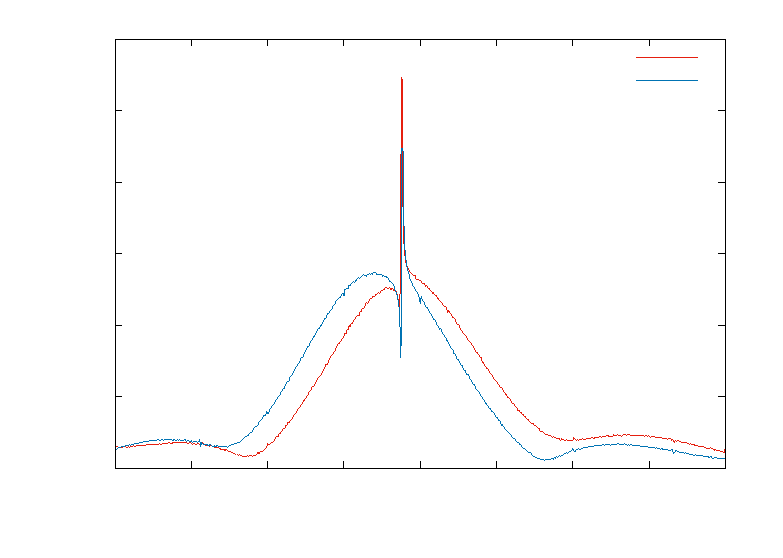
\includegraphics{plots/Pulsandcollect138}}%
    \gplfronttext
  \end{picture}%
\endgroup

    \caption[]{ask: what is the peak corresponding? hydrogen signal? -> yes}
    \label{fig:Pulsandcollect}
\end{figure}



\begin{figure}[H]
    \centering
    % GNUPLOT: LaTeX picture with Postscript
\begingroup
  % Encoding inside the plot.  In the header of your document, this encoding
  % should to defined, e.g., by using
  % \usepackage[cp1252,<other encodings>]{inputenc}
  \inputencoding{cp1252}%
  \makeatletter
  \providecommand\color[2][]{%
    \GenericError{(gnuplot) \space\space\space\@spaces}{%
      Package color not loaded in conjunction with
      terminal option `colourtext'%
    }{See the gnuplot documentation for explanation.%
    }{Either use 'blacktext' in gnuplot or load the package
      color.sty in LaTeX.}%
    \renewcommand\color[2][]{}%
  }%
  \providecommand\includegraphics[2][]{%
    \GenericError{(gnuplot) \space\space\space\@spaces}{%
      Package graphicx or graphics not loaded%
    }{See the gnuplot documentation for explanation.%
    }{The gnuplot epslatex terminal needs graphicx.sty or graphics.sty.}%
    \renewcommand\includegraphics[2][]{}%
  }%
  \providecommand\rotatebox[2]{#2}%
  \@ifundefined{ifGPcolor}{%
    \newif\ifGPcolor
    \GPcolorfalse
  }{}%
  \@ifundefined{ifGPblacktext}{%
    \newif\ifGPblacktext
    \GPblacktexttrue
  }{}%
  % define a \g@addto@macro without @ in the name:
  \let\gplgaddtomacro\g@addto@macro
  % define empty templates for all commands taking text:
  \gdef\gplbacktext{}%
  \gdef\gplfronttext{}%
  \makeatother
  \ifGPblacktext
    % no textcolor at all
    \def\colorrgb#1{}%
    \def\colorgray#1{}%
  \else
    % gray or color?
    \ifGPcolor
      \def\colorrgb#1{\color[rgb]{#1}}%
      \def\colorgray#1{\color[gray]{#1}}%
      \expandafter\def\csname LTw\endcsname{\color{white}}%
      \expandafter\def\csname LTb\endcsname{\color{black}}%
      \expandafter\def\csname LTa\endcsname{\color{black}}%
      \expandafter\def\csname LT0\endcsname{\color[rgb]{1,0,0}}%
      \expandafter\def\csname LT1\endcsname{\color[rgb]{0,1,0}}%
      \expandafter\def\csname LT2\endcsname{\color[rgb]{0,0,1}}%
      \expandafter\def\csname LT3\endcsname{\color[rgb]{1,0,1}}%
      \expandafter\def\csname LT4\endcsname{\color[rgb]{0,1,1}}%
      \expandafter\def\csname LT5\endcsname{\color[rgb]{1,1,0}}%
      \expandafter\def\csname LT6\endcsname{\color[rgb]{0,0,0}}%
      \expandafter\def\csname LT7\endcsname{\color[rgb]{1,0.3,0}}%
      \expandafter\def\csname LT8\endcsname{\color[rgb]{0.5,0.5,0.5}}%
    \else
      % gray
      \def\colorrgb#1{\color{black}}%
      \def\colorgray#1{\color[gray]{#1}}%
      \expandafter\def\csname LTw\endcsname{\color{white}}%
      \expandafter\def\csname LTb\endcsname{\color{black}}%
      \expandafter\def\csname LTa\endcsname{\color{black}}%
      \expandafter\def\csname LT0\endcsname{\color{black}}%
      \expandafter\def\csname LT1\endcsname{\color{black}}%
      \expandafter\def\csname LT2\endcsname{\color{black}}%
      \expandafter\def\csname LT3\endcsname{\color{black}}%
      \expandafter\def\csname LT4\endcsname{\color{black}}%
      \expandafter\def\csname LT5\endcsname{\color{black}}%
      \expandafter\def\csname LT6\endcsname{\color{black}}%
      \expandafter\def\csname LT7\endcsname{\color{black}}%
      \expandafter\def\csname LT8\endcsname{\color{black}}%
    \fi
  \fi
    \setlength{\unitlength}{0.0500bp}%
    \ifx\gptboxheight\undefined%
      \newlength{\gptboxheight}%
      \newlength{\gptboxwidth}%
      \newsavebox{\gptboxtext}%
    \fi%
    \setlength{\fboxrule}{0.5pt}%
    \setlength{\fboxsep}{1pt}%
\begin{picture}(7200.00,5040.00)%
    \gplgaddtomacro\gplbacktext{%
      \csname LTb\endcsname%%
      \put(682,704){\makebox(0,0)[r]{\strut{}$0$}}%
      \put(682,1161){\makebox(0,0)[r]{\strut{}$10$}}%
      \put(682,1618){\makebox(0,0)[r]{\strut{}$20$}}%
      \put(682,2076){\makebox(0,0)[r]{\strut{}$30$}}%
      \put(682,2533){\makebox(0,0)[r]{\strut{}$40$}}%
      \put(682,2990){\makebox(0,0)[r]{\strut{}$50$}}%
      \put(682,3447){\makebox(0,0)[r]{\strut{}$60$}}%
      \put(682,3905){\makebox(0,0)[r]{\strut{}$70$}}%
      \put(682,4362){\makebox(0,0)[r]{\strut{}$80$}}%
      \put(682,4819){\makebox(0,0)[r]{\strut{}$90$}}%
      \put(814,484){\makebox(0,0){\strut{}$1830$}}%
      \put(1613,484){\makebox(0,0){\strut{}$1832$}}%
      \put(2411,484){\makebox(0,0){\strut{}$1834$}}%
      \put(3210,484){\makebox(0,0){\strut{}$1836$}}%
      \put(4008,484){\makebox(0,0){\strut{}$1838$}}%
      \put(4807,484){\makebox(0,0){\strut{}$1840$}}%
      \put(5605,484){\makebox(0,0){\strut{}$1842$}}%
      \put(6404,484){\makebox(0,0){\strut{}$1844$}}%
      \put(4208,2304){\makebox(0,0)[l]{\strut{}FWHM $= \SI{1.177 \pm 0.042}{\hertz}$}}%
      \put(4208,2762){\makebox(0,0)[l]{\strut{}$\sigma =  \SI{0.500 \pm 0.018}{\hertz}$}}%
    }%
    \gplgaddtomacro\gplfronttext{%
      \csname LTb\endcsname%%
      \put(209,2761){\rotatebox{-270}{\makebox(0,0){\strut{}Amplitude in $\si{\mu \volt}$}}}%
      \put(3808,154){\makebox(0,0){\strut{}Frequency in $\si{\hertz}$}}%
      \csname LTb\endcsname%%
      \put(5816,4646){\makebox(0,0)[r]{\strut{}magnitude spectrum}}%
      \csname LTb\endcsname%%
      \put(5816,4426){\makebox(0,0)[r]{\strut{}voigt-profile}}%
      \csname LTb\endcsname%%
      \put(5816,4206){\makebox(0,0)[r]{\strut{}\textsc{Gauss}-Fit}}%
    }%
    \gplbacktext
    \put(0,0){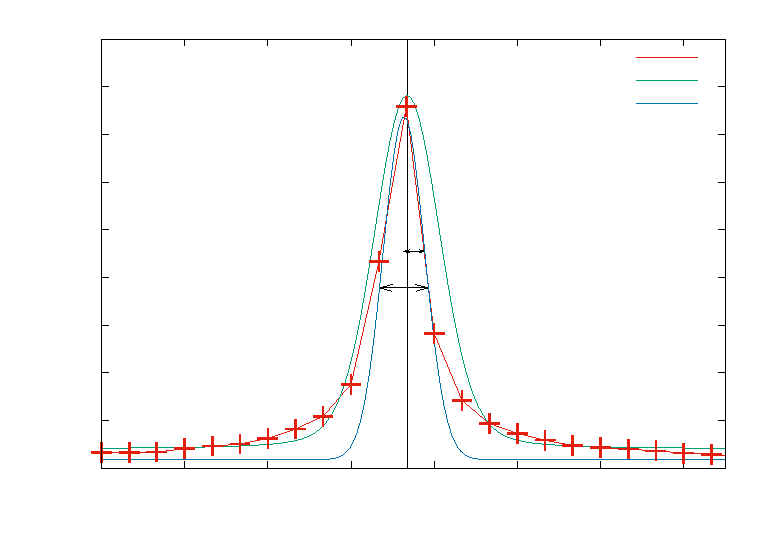
\includegraphics{plots/Pulsandcollect138_delay_25_gauss}}%
    \gplfronttext
  \end{picture}%
\endgroup

    \caption[]{ask: gauss or voigt. this is gauss -> both\newline
    longer acquisition \SI{25}{\milli \second} -> only hydrogen siganal? is the peak the same than in the previous diagramm?  -> yes\newline
    integral under curve with our measured fit? -> try to find soemthing, try shorter range and more points\newline
    signal to noise ratio: what to do? -> magnitude, which unit is the amplitude, tutor will send us an email, try back fouriertransform (only keep real values)
    \\
    calculate: amplitude; crossbar for datapoints\\
    sometimes 1/e sometimes 1/2 -> definition}
    \label{fig:Pulsandcollect138_delay_25_gauss}
\end{figure}
\begin{figure}[H]
    \centering
    % GNUPLOT: LaTeX picture with Postscript
\begingroup
  % Encoding inside the plot.  In the header of your document, this encoding
  % should to defined, e.g., by using
  % \usepackage[cp1252,<other encodings>]{inputenc}
  \inputencoding{cp1252}%
  \makeatletter
  \providecommand\color[2][]{%
    \GenericError{(gnuplot) \space\space\space\@spaces}{%
      Package color not loaded in conjunction with
      terminal option `colourtext'%
    }{See the gnuplot documentation for explanation.%
    }{Either use 'blacktext' in gnuplot or load the package
      color.sty in LaTeX.}%
    \renewcommand\color[2][]{}%
  }%
  \providecommand\includegraphics[2][]{%
    \GenericError{(gnuplot) \space\space\space\@spaces}{%
      Package graphicx or graphics not loaded%
    }{See the gnuplot documentation for explanation.%
    }{The gnuplot epslatex terminal needs graphicx.sty or graphics.sty.}%
    \renewcommand\includegraphics[2][]{}%
  }%
  \providecommand\rotatebox[2]{#2}%
  \@ifundefined{ifGPcolor}{%
    \newif\ifGPcolor
    \GPcolorfalse
  }{}%
  \@ifundefined{ifGPblacktext}{%
    \newif\ifGPblacktext
    \GPblacktexttrue
  }{}%
  % define a \g@addto@macro without @ in the name:
  \let\gplgaddtomacro\g@addto@macro
  % define empty templates for all commands taking text:
  \gdef\gplbacktext{}%
  \gdef\gplfronttext{}%
  \makeatother
  \ifGPblacktext
    % no textcolor at all
    \def\colorrgb#1{}%
    \def\colorgray#1{}%
  \else
    % gray or color?
    \ifGPcolor
      \def\colorrgb#1{\color[rgb]{#1}}%
      \def\colorgray#1{\color[gray]{#1}}%
      \expandafter\def\csname LTw\endcsname{\color{white}}%
      \expandafter\def\csname LTb\endcsname{\color{black}}%
      \expandafter\def\csname LTa\endcsname{\color{black}}%
      \expandafter\def\csname LT0\endcsname{\color[rgb]{1,0,0}}%
      \expandafter\def\csname LT1\endcsname{\color[rgb]{0,1,0}}%
      \expandafter\def\csname LT2\endcsname{\color[rgb]{0,0,1}}%
      \expandafter\def\csname LT3\endcsname{\color[rgb]{1,0,1}}%
      \expandafter\def\csname LT4\endcsname{\color[rgb]{0,1,1}}%
      \expandafter\def\csname LT5\endcsname{\color[rgb]{1,1,0}}%
      \expandafter\def\csname LT6\endcsname{\color[rgb]{0,0,0}}%
      \expandafter\def\csname LT7\endcsname{\color[rgb]{1,0.3,0}}%
      \expandafter\def\csname LT8\endcsname{\color[rgb]{0.5,0.5,0.5}}%
    \else
      % gray
      \def\colorrgb#1{\color{black}}%
      \def\colorgray#1{\color[gray]{#1}}%
      \expandafter\def\csname LTw\endcsname{\color{white}}%
      \expandafter\def\csname LTb\endcsname{\color{black}}%
      \expandafter\def\csname LTa\endcsname{\color{black}}%
      \expandafter\def\csname LT0\endcsname{\color{black}}%
      \expandafter\def\csname LT1\endcsname{\color{black}}%
      \expandafter\def\csname LT2\endcsname{\color{black}}%
      \expandafter\def\csname LT3\endcsname{\color{black}}%
      \expandafter\def\csname LT4\endcsname{\color{black}}%
      \expandafter\def\csname LT5\endcsname{\color{black}}%
      \expandafter\def\csname LT6\endcsname{\color{black}}%
      \expandafter\def\csname LT7\endcsname{\color{black}}%
      \expandafter\def\csname LT8\endcsname{\color{black}}%
    \fi
  \fi
    \setlength{\unitlength}{0.0500bp}%
    \ifx\gptboxheight\undefined%
      \newlength{\gptboxheight}%
      \newlength{\gptboxwidth}%
      \newsavebox{\gptboxtext}%
    \fi%
    \setlength{\fboxrule}{0.5pt}%
    \setlength{\fboxsep}{1pt}%
\begin{picture}(7200.00,5040.00)%
    \gplgaddtomacro\gplbacktext{%
      \csname LTb\endcsname%%
      \put(682,704){\makebox(0,0)[r]{\strut{}$0$}}%
      \put(682,1161){\makebox(0,0)[r]{\strut{}$10$}}%
      \put(682,1618){\makebox(0,0)[r]{\strut{}$20$}}%
      \put(682,2076){\makebox(0,0)[r]{\strut{}$30$}}%
      \put(682,2533){\makebox(0,0)[r]{\strut{}$40$}}%
      \put(682,2990){\makebox(0,0)[r]{\strut{}$50$}}%
      \put(682,3447){\makebox(0,0)[r]{\strut{}$60$}}%
      \put(682,3905){\makebox(0,0)[r]{\strut{}$70$}}%
      \put(682,4362){\makebox(0,0)[r]{\strut{}$80$}}%
      \put(682,4819){\makebox(0,0)[r]{\strut{}$90$}}%
      \put(814,484){\makebox(0,0){\strut{}$1830$}}%
      \put(1613,484){\makebox(0,0){\strut{}$1832$}}%
      \put(2411,484){\makebox(0,0){\strut{}$1834$}}%
      \put(3210,484){\makebox(0,0){\strut{}$1836$}}%
      \put(4008,484){\makebox(0,0){\strut{}$1838$}}%
      \put(4807,484){\makebox(0,0){\strut{}$1840$}}%
      \put(5605,484){\makebox(0,0){\strut{}$1842$}}%
      \put(6404,484){\makebox(0,0){\strut{}$1844$}}%
    }%
    \gplgaddtomacro\gplfronttext{%
      \csname LTb\endcsname%%
      \put(209,2761){\rotatebox{-270}{\makebox(0,0){\strut{}Amplitude}}}%
      \put(3808,154){\makebox(0,0){\strut{}Frequency in $\si{\hertz}$}}%
      \csname LTb\endcsname%%
      \put(5816,4646){\makebox(0,0)[r]{\strut{}magnitude spectrum}}%
      \csname LTb\endcsname%%
      \put(5816,4426){\makebox(0,0)[r]{\strut{}voigt-profile}}%
    }%
    \gplbacktext
    \put(0,0){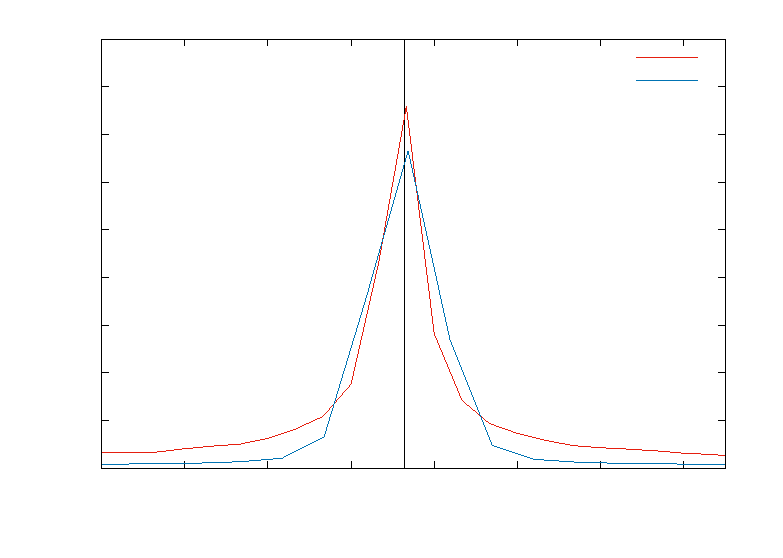
\includegraphics{plots/Pulsandcollect138_delay_25_voigt}}%
    \gplfronttext
  \end{picture}%
\endgroup

    \caption[]{ask: gauss or voigt. this is voigt}
    \label{fig:PulsandcollePulsandcollect138_delay_25_voigtctlangerdelay}
\end{figure}

\textcolor{red}{real and imaginary signal -> explain it}
% !TEX root = main.tex
\section{Longitudinal relaxation measurements T1}
\label{sec:LongitudinalrelaxationmeasurementsT1}
To measure the longitudinal spin lattice relaxation exist two possibilities. The first we want to have a closer look at is the measurement via $\tau_p$ (polarizing pulse duration). Therefore the computer program \textit{Prospa} applies a polarizing pulse orthogonal to the earths magentic field. Due to this polarizing pulse the spins align in the transversal plain and form a bulk magnetisation. By time the magnetisation becomes stronger, therefore the signal becomes stronger. This relation is visualized in the figure \ref{fig:BildT1}.

\begin{figure}[H]
    \centering
    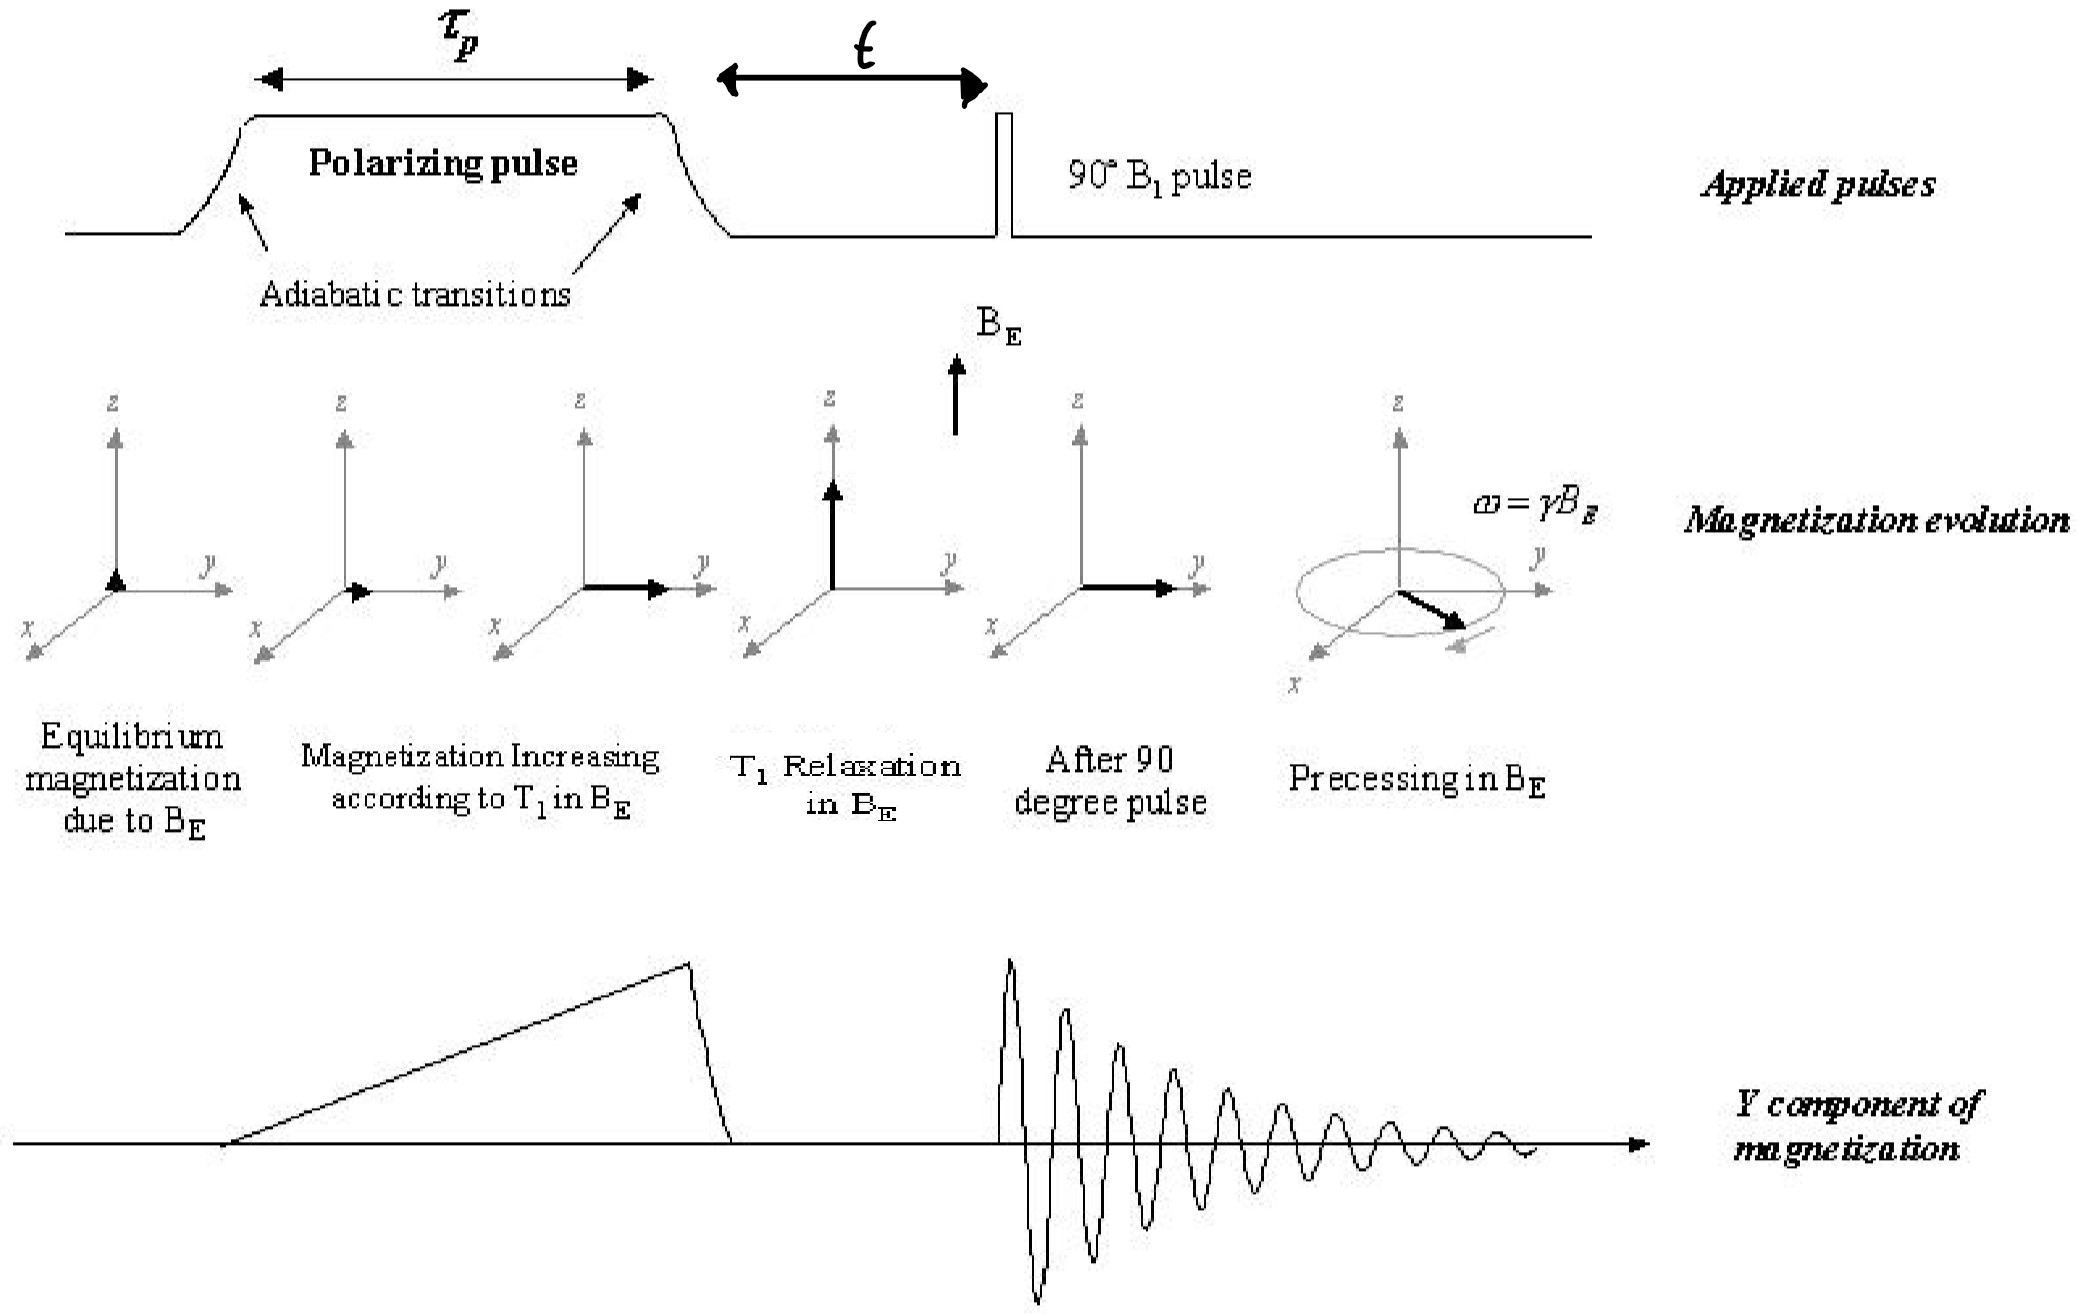
\includegraphics[width= \textwidth]{BildT1.png}   
    \caption[Sketch to show how T$_1$ can be measured. \cite{Bild}]{Sketch to show how T$_1$ can be measured. One way is by changing the polarizing pulse duration $\tau_p$ and the other way is by variy the time between the polarizing pulse and the \SI{90}{\degree} pulse. \cite{Bild}}
    \label{fig:BildT1}
\end{figure}

Due to the increasing magnetisation it is possible to calculate the T$_{1,p}$ relaxation. In order to do so the magnetisation time is increased step by step from \SI{500}{\milli \second} to \SI{4500}{\milli \second} in step sizes of \SI{500}{\milli \second} and in each configuration the signal maximum is calculated of the fourie transformed spectrum. Figure \ref{fig:T1Polarisationsfeldfeld} shows the attenuation of the signals normalized to the maximum peak E$_0$. The reason of that is that by applying a fit function as followed:
\begin{align}
    S(x)=S_0 \cdot [1-exp(\frac{-x}{T_{1,p}})] \ ,
    \label{eq: fitBp}
\end{align}
it is possible to calculate the relaxation time T$_{1,p}$. The exponential decay is a result of loss of phase coherence between the spins and will be used for every measurement of spin relaxation. In this case T$_{1,p}$ is \SI{2912.8800 \pm 0.0048}{\milli \second}.

\begin{figure}[H]
    \centering
    % GNUPLOT: LaTeX picture with Postscript
\begingroup
  % Encoding inside the plot.  In the header of your document, this encoding
  % should to defined, e.g., by using
  % \usepackage[cp1252,<other encodings>]{inputenc}
  \inputencoding{cp1252}%
  \makeatletter
  \providecommand\color[2][]{%
    \GenericError{(gnuplot) \space\space\space\@spaces}{%
      Package color not loaded in conjunction with
      terminal option `colourtext'%
    }{See the gnuplot documentation for explanation.%
    }{Either use 'blacktext' in gnuplot or load the package
      color.sty in LaTeX.}%
    \renewcommand\color[2][]{}%
  }%
  \providecommand\includegraphics[2][]{%
    \GenericError{(gnuplot) \space\space\space\@spaces}{%
      Package graphicx or graphics not loaded%
    }{See the gnuplot documentation for explanation.%
    }{The gnuplot epslatex terminal needs graphicx.sty or graphics.sty.}%
    \renewcommand\includegraphics[2][]{}%
  }%
  \providecommand\rotatebox[2]{#2}%
  \@ifundefined{ifGPcolor}{%
    \newif\ifGPcolor
    \GPcolorfalse
  }{}%
  \@ifundefined{ifGPblacktext}{%
    \newif\ifGPblacktext
    \GPblacktexttrue
  }{}%
  % define a \g@addto@macro without @ in the name:
  \let\gplgaddtomacro\g@addto@macro
  % define empty templates for all commands taking text:
  \gdef\gplbacktext{}%
  \gdef\gplfronttext{}%
  \makeatother
  \ifGPblacktext
    % no textcolor at all
    \def\colorrgb#1{}%
    \def\colorgray#1{}%
  \else
    % gray or color?
    \ifGPcolor
      \def\colorrgb#1{\color[rgb]{#1}}%
      \def\colorgray#1{\color[gray]{#1}}%
      \expandafter\def\csname LTw\endcsname{\color{white}}%
      \expandafter\def\csname LTb\endcsname{\color{black}}%
      \expandafter\def\csname LTa\endcsname{\color{black}}%
      \expandafter\def\csname LT0\endcsname{\color[rgb]{1,0,0}}%
      \expandafter\def\csname LT1\endcsname{\color[rgb]{0,1,0}}%
      \expandafter\def\csname LT2\endcsname{\color[rgb]{0,0,1}}%
      \expandafter\def\csname LT3\endcsname{\color[rgb]{1,0,1}}%
      \expandafter\def\csname LT4\endcsname{\color[rgb]{0,1,1}}%
      \expandafter\def\csname LT5\endcsname{\color[rgb]{1,1,0}}%
      \expandafter\def\csname LT6\endcsname{\color[rgb]{0,0,0}}%
      \expandafter\def\csname LT7\endcsname{\color[rgb]{1,0.3,0}}%
      \expandafter\def\csname LT8\endcsname{\color[rgb]{0.5,0.5,0.5}}%
    \else
      % gray
      \def\colorrgb#1{\color{black}}%
      \def\colorgray#1{\color[gray]{#1}}%
      \expandafter\def\csname LTw\endcsname{\color{white}}%
      \expandafter\def\csname LTb\endcsname{\color{black}}%
      \expandafter\def\csname LTa\endcsname{\color{black}}%
      \expandafter\def\csname LT0\endcsname{\color{black}}%
      \expandafter\def\csname LT1\endcsname{\color{black}}%
      \expandafter\def\csname LT2\endcsname{\color{black}}%
      \expandafter\def\csname LT3\endcsname{\color{black}}%
      \expandafter\def\csname LT4\endcsname{\color{black}}%
      \expandafter\def\csname LT5\endcsname{\color{black}}%
      \expandafter\def\csname LT6\endcsname{\color{black}}%
      \expandafter\def\csname LT7\endcsname{\color{black}}%
      \expandafter\def\csname LT8\endcsname{\color{black}}%
    \fi
  \fi
    \setlength{\unitlength}{0.0500bp}%
    \ifx\gptboxheight\undefined%
      \newlength{\gptboxheight}%
      \newlength{\gptboxwidth}%
      \newsavebox{\gptboxtext}%
    \fi%
    \setlength{\fboxrule}{0.5pt}%
    \setlength{\fboxsep}{1pt}%
\begin{picture}(7200.00,5040.00)%
    \gplgaddtomacro\gplbacktext{%
      \csname LTb\endcsname%%
      \put(814,704){\makebox(0,0)[r]{\strut{}$0$}}%
      \put(814,1527){\makebox(0,0)[r]{\strut{}$0.2$}}%
      \put(814,2350){\makebox(0,0)[r]{\strut{}$0.4$}}%
      \put(814,3173){\makebox(0,0)[r]{\strut{}$0.6$}}%
      \put(814,3996){\makebox(0,0)[r]{\strut{}$0.8$}}%
      \put(814,4819){\makebox(0,0)[r]{\strut{}$1$}}%
      \put(946,484){\makebox(0,0){\strut{}$0$}}%
      \put(1660,484){\makebox(0,0){\strut{}$500$}}%
      \put(2375,484){\makebox(0,0){\strut{}$1000$}}%
      \put(3089,484){\makebox(0,0){\strut{}$1500$}}%
      \put(3803,484){\makebox(0,0){\strut{}$2000$}}%
      \put(4517,484){\makebox(0,0){\strut{}$2500$}}%
      \put(5232,484){\makebox(0,0){\strut{}$3000$}}%
      \put(5946,484){\makebox(0,0){\strut{}$3500$}}%
      \put(6660,484){\makebox(0,0){\strut{}$4000$}}%
    }%
    \gplgaddtomacro\gplfronttext{%
      \csname LTb\endcsname%%
      \put(209,2761){\rotatebox{-270}{\makebox(0,0){\strut{}Attenuation $\frac{\text{E}}{\text{E}_0}$}}}%
      \put(3874,154){\makebox(0,0){\strut{}Time in $\si{\milli \second}$}}%
      \csname LTb\endcsname%%
      \put(5816,4646){\makebox(0,0)[r]{\strut{}measured values$ }}%
      \csname LTb\endcsname%%
      \put(5816,4426){\makebox(0,0)[r]{\strut{}attenuation-Fit}}%
    }%
    \gplbacktext
    \put(0,0){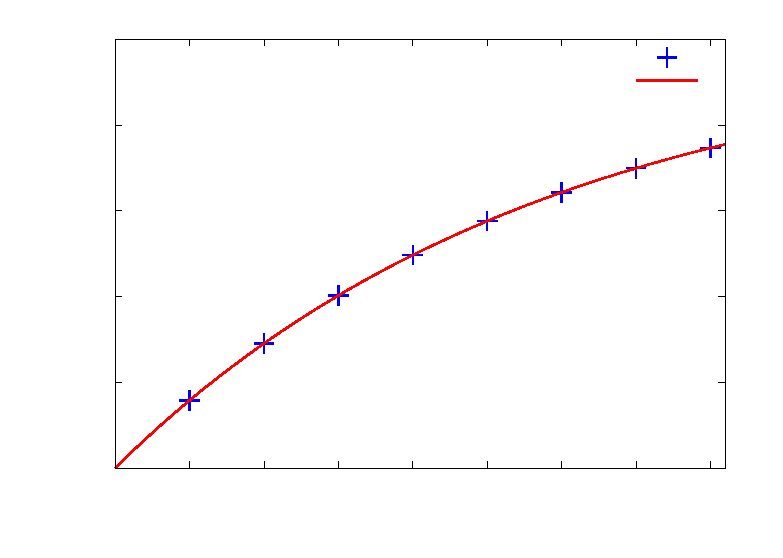
\includegraphics{plots/T1Polarisationsfeldfeld}}%
    \gplfronttext
  \end{picture}%
\endgroup

    \caption[T$_{1,p}$ measurement by variy $\tau_p$ and see how the attenuation $\frac{\text{E}}{\text{E}_0}$ evolves.]{T$_{1,p}$ measurement by variy $\tau_p$ and see how the attenuation $\frac{\text{E}}{\text{E}_0}$ evolves. The provided exponential fit results in a value for T$_{1,p}$ of \SI{2912.8800 \pm 0.0048}{\milli \second}.}
    \label{fig:T1Polarisationsfeldfeld}
\end{figure}

The second option is to calculate the spin lattice relaxation via the earths magneitc field B$_e$. In this case the index will be $e$ for the spin lattice relaxation. The procedure in this case is to change the time $t$ (pre-90 minimum delay) between the polarizing pulse ends and the \SI{90}{\degree} pulse beginns. This relation is also visualized in the figure \ref{fig:BildT1}. The pre-90 minimum delay is chosen as \SI{0}{\milli \second} and the pre-90 delay step size \SI{500}{\milli \second}. For every configuration the signal maximum is calculated again of the fourie transformed spectrum. Figure \ref{fig:T1Erdmagnetfeld} shows the attenuation of the signals normalized to the maximum peak E$_0$. This time the T$_{1,e}$ can be calculated by following fit function:
\begin{align}
    S(x) = S_0 \cdot exp(\frac{-x}{T_{1,e}}) \ .
    \label{eq: fitBe}
\end{align}
For our case T$_{1,e}$ is \SI{2753.0500 \pm 0.0012}{\milli \second}.\newline
In both ways the uncertainty of the T$_1$ values are really small. This is the result of really good align values to the fit function. Nevertheless T$_{1,p}$ and T$_{1,e}$ are not consistent even though the uncertainty is considered. This might be, due to the fact that those to measurements are based on two different methods and there can always be differences in the setup \textcolor{red}{genauer anschauen}. Even though they are not consistent, the values for T$_{1,p}$ and T$_{1,e}$ have the same magnitude.
\begin{figure}[H]
    \centering
    % GNUPLOT: LaTeX picture with Postscript
\begingroup
  % Encoding inside the plot.  In the header of your document, this encoding
  % should to defined, e.g., by using
  % \usepackage[cp1252,<other encodings>]{inputenc}
  \inputencoding{cp1252}%
  \makeatletter
  \providecommand\color[2][]{%
    \GenericError{(gnuplot) \space\space\space\@spaces}{%
      Package color not loaded in conjunction with
      terminal option `colourtext'%
    }{See the gnuplot documentation for explanation.%
    }{Either use 'blacktext' in gnuplot or load the package
      color.sty in LaTeX.}%
    \renewcommand\color[2][]{}%
  }%
  \providecommand\includegraphics[2][]{%
    \GenericError{(gnuplot) \space\space\space\@spaces}{%
      Package graphicx or graphics not loaded%
    }{See the gnuplot documentation for explanation.%
    }{The gnuplot epslatex terminal needs graphicx.sty or graphics.sty.}%
    \renewcommand\includegraphics[2][]{}%
  }%
  \providecommand\rotatebox[2]{#2}%
  \@ifundefined{ifGPcolor}{%
    \newif\ifGPcolor
    \GPcolorfalse
  }{}%
  \@ifundefined{ifGPblacktext}{%
    \newif\ifGPblacktext
    \GPblacktexttrue
  }{}%
  % define a \g@addto@macro without @ in the name:
  \let\gplgaddtomacro\g@addto@macro
  % define empty templates for all commands taking text:
  \gdef\gplbacktext{}%
  \gdef\gplfronttext{}%
  \makeatother
  \ifGPblacktext
    % no textcolor at all
    \def\colorrgb#1{}%
    \def\colorgray#1{}%
  \else
    % gray or color?
    \ifGPcolor
      \def\colorrgb#1{\color[rgb]{#1}}%
      \def\colorgray#1{\color[gray]{#1}}%
      \expandafter\def\csname LTw\endcsname{\color{white}}%
      \expandafter\def\csname LTb\endcsname{\color{black}}%
      \expandafter\def\csname LTa\endcsname{\color{black}}%
      \expandafter\def\csname LT0\endcsname{\color[rgb]{1,0,0}}%
      \expandafter\def\csname LT1\endcsname{\color[rgb]{0,1,0}}%
      \expandafter\def\csname LT2\endcsname{\color[rgb]{0,0,1}}%
      \expandafter\def\csname LT3\endcsname{\color[rgb]{1,0,1}}%
      \expandafter\def\csname LT4\endcsname{\color[rgb]{0,1,1}}%
      \expandafter\def\csname LT5\endcsname{\color[rgb]{1,1,0}}%
      \expandafter\def\csname LT6\endcsname{\color[rgb]{0,0,0}}%
      \expandafter\def\csname LT7\endcsname{\color[rgb]{1,0.3,0}}%
      \expandafter\def\csname LT8\endcsname{\color[rgb]{0.5,0.5,0.5}}%
    \else
      % gray
      \def\colorrgb#1{\color{black}}%
      \def\colorgray#1{\color[gray]{#1}}%
      \expandafter\def\csname LTw\endcsname{\color{white}}%
      \expandafter\def\csname LTb\endcsname{\color{black}}%
      \expandafter\def\csname LTa\endcsname{\color{black}}%
      \expandafter\def\csname LT0\endcsname{\color{black}}%
      \expandafter\def\csname LT1\endcsname{\color{black}}%
      \expandafter\def\csname LT2\endcsname{\color{black}}%
      \expandafter\def\csname LT3\endcsname{\color{black}}%
      \expandafter\def\csname LT4\endcsname{\color{black}}%
      \expandafter\def\csname LT5\endcsname{\color{black}}%
      \expandafter\def\csname LT6\endcsname{\color{black}}%
      \expandafter\def\csname LT7\endcsname{\color{black}}%
      \expandafter\def\csname LT8\endcsname{\color{black}}%
    \fi
  \fi
    \setlength{\unitlength}{0.0500bp}%
    \ifx\gptboxheight\undefined%
      \newlength{\gptboxheight}%
      \newlength{\gptboxwidth}%
      \newsavebox{\gptboxtext}%
    \fi%
    \setlength{\fboxrule}{0.5pt}%
    \setlength{\fboxsep}{1pt}%
\begin{picture}(7200.00,5040.00)%
    \gplgaddtomacro\gplbacktext{%
      \csname LTb\endcsname%%
      \put(814,704){\makebox(0,0)[r]{\strut{}$0$}}%
      \put(814,1527){\makebox(0,0)[r]{\strut{}$0.2$}}%
      \put(814,2350){\makebox(0,0)[r]{\strut{}$0.4$}}%
      \put(814,3173){\makebox(0,0)[r]{\strut{}$0.6$}}%
      \put(814,3996){\makebox(0,0)[r]{\strut{}$0.8$}}%
      \put(814,4819){\makebox(0,0)[r]{\strut{}$1$}}%
      \put(946,484){\makebox(0,0){\strut{}$0$}}%
      \put(1660,484){\makebox(0,0){\strut{}$500$}}%
      \put(2375,484){\makebox(0,0){\strut{}$1000$}}%
      \put(3089,484){\makebox(0,0){\strut{}$1500$}}%
      \put(3803,484){\makebox(0,0){\strut{}$2000$}}%
      \put(4517,484){\makebox(0,0){\strut{}$2500$}}%
      \put(5232,484){\makebox(0,0){\strut{}$3000$}}%
      \put(5946,484){\makebox(0,0){\strut{}$3500$}}%
      \put(6660,484){\makebox(0,0){\strut{}$4000$}}%
    }%
    \gplgaddtomacro\gplfronttext{%
      \csname LTb\endcsname%%
      \put(209,2761){\rotatebox{-270}{\makebox(0,0){\strut{}Attenuation $\frac{\text{E}}{\text{E}_0}$}}}%
      \put(3874,154){\makebox(0,0){\strut{}Time between pulses $t$ in $\si{\milli \second}$}}%
      \csname LTb\endcsname%%
      \put(5816,4646){\makebox(0,0)[r]{\strut{}measured values}}%
      \csname LTb\endcsname%%
      \put(5816,4426){\makebox(0,0)[r]{\strut{}attenuation-Fit}}%
    }%
    \gplbacktext
    \put(0,0){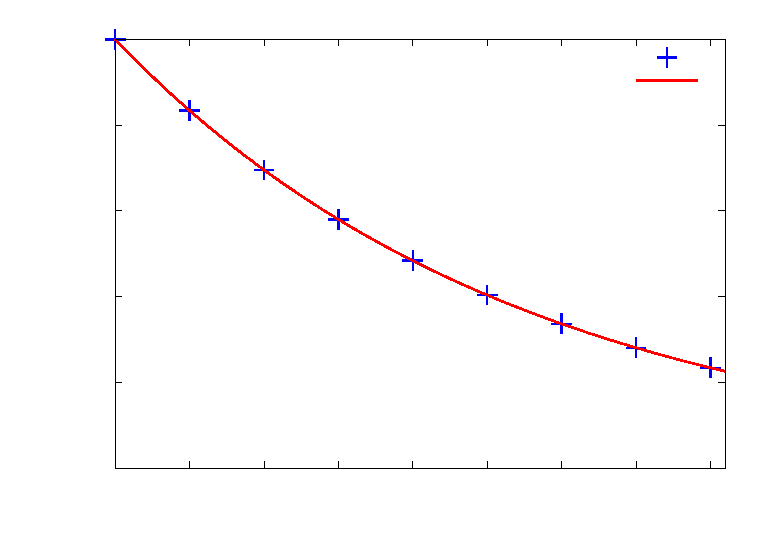
\includegraphics{plots/T1Erdmagnetfeld}}%
    \gplfronttext
  \end{picture}%
\endgroup

    \caption[T$_{1,e}$ measurement by variy $t$ and see how the attenuation $\frac{\text{E}}{\text{E}_0}$ evolves.]{T$_{1,e}$ measurement by variy $t$ and see how the attenuation $\frac{\text{E}}{\text{E}_0}$ evolves. The provided exponential fit results in a value for T$_{1,e}$ of \SI{2753.0500 \pm 0.0012}{\milli \second}.}
    \label{fig:T1Erdmagnetfeld}
\end{figure}

% !TEX root = main.tex
\section{Hahn echo}
\label{sec:Hahnecho}



\begin{figure}[H]
    \centering
    % GNUPLOT: LaTeX picture with Postscript
\begingroup
  % Encoding inside the plot.  In the header of your document, this encoding
  % should to defined, e.g., by using
  % \usepackage[cp1252,<other encodings>]{inputenc}
  \inputencoding{cp1252}%
  \makeatletter
  \providecommand\color[2][]{%
    \GenericError{(gnuplot) \space\space\space\@spaces}{%
      Package color not loaded in conjunction with
      terminal option `colourtext'%
    }{See the gnuplot documentation for explanation.%
    }{Either use 'blacktext' in gnuplot or load the package
      color.sty in LaTeX.}%
    \renewcommand\color[2][]{}%
  }%
  \providecommand\includegraphics[2][]{%
    \GenericError{(gnuplot) \space\space\space\@spaces}{%
      Package graphicx or graphics not loaded%
    }{See the gnuplot documentation for explanation.%
    }{The gnuplot epslatex terminal needs graphicx.sty or graphics.sty.}%
    \renewcommand\includegraphics[2][]{}%
  }%
  \providecommand\rotatebox[2]{#2}%
  \@ifundefined{ifGPcolor}{%
    \newif\ifGPcolor
    \GPcolorfalse
  }{}%
  \@ifundefined{ifGPblacktext}{%
    \newif\ifGPblacktext
    \GPblacktexttrue
  }{}%
  % define a \g@addto@macro without @ in the name:
  \let\gplgaddtomacro\g@addto@macro
  % define empty templates for all commands taking text:
  \gdef\gplbacktext{}%
  \gdef\gplfronttext{}%
  \makeatother
  \ifGPblacktext
    % no textcolor at all
    \def\colorrgb#1{}%
    \def\colorgray#1{}%
  \else
    % gray or color?
    \ifGPcolor
      \def\colorrgb#1{\color[rgb]{#1}}%
      \def\colorgray#1{\color[gray]{#1}}%
      \expandafter\def\csname LTw\endcsname{\color{white}}%
      \expandafter\def\csname LTb\endcsname{\color{black}}%
      \expandafter\def\csname LTa\endcsname{\color{black}}%
      \expandafter\def\csname LT0\endcsname{\color[rgb]{1,0,0}}%
      \expandafter\def\csname LT1\endcsname{\color[rgb]{0,1,0}}%
      \expandafter\def\csname LT2\endcsname{\color[rgb]{0,0,1}}%
      \expandafter\def\csname LT3\endcsname{\color[rgb]{1,0,1}}%
      \expandafter\def\csname LT4\endcsname{\color[rgb]{0,1,1}}%
      \expandafter\def\csname LT5\endcsname{\color[rgb]{1,1,0}}%
      \expandafter\def\csname LT6\endcsname{\color[rgb]{0,0,0}}%
      \expandafter\def\csname LT7\endcsname{\color[rgb]{1,0.3,0}}%
      \expandafter\def\csname LT8\endcsname{\color[rgb]{0.5,0.5,0.5}}%
    \else
      % gray
      \def\colorrgb#1{\color{black}}%
      \def\colorgray#1{\color[gray]{#1}}%
      \expandafter\def\csname LTw\endcsname{\color{white}}%
      \expandafter\def\csname LTb\endcsname{\color{black}}%
      \expandafter\def\csname LTa\endcsname{\color{black}}%
      \expandafter\def\csname LT0\endcsname{\color{black}}%
      \expandafter\def\csname LT1\endcsname{\color{black}}%
      \expandafter\def\csname LT2\endcsname{\color{black}}%
      \expandafter\def\csname LT3\endcsname{\color{black}}%
      \expandafter\def\csname LT4\endcsname{\color{black}}%
      \expandafter\def\csname LT5\endcsname{\color{black}}%
      \expandafter\def\csname LT6\endcsname{\color{black}}%
      \expandafter\def\csname LT7\endcsname{\color{black}}%
      \expandafter\def\csname LT8\endcsname{\color{black}}%
    \fi
  \fi
    \setlength{\unitlength}{0.0500bp}%
    \ifx\gptboxheight\undefined%
      \newlength{\gptboxheight}%
      \newlength{\gptboxwidth}%
      \newsavebox{\gptboxtext}%
    \fi%
    \setlength{\fboxrule}{0.5pt}%
    \setlength{\fboxsep}{1pt}%
\begin{picture}(7200.00,5040.00)%
    \gplgaddtomacro\gplbacktext{%
      \csname LTb\endcsname%%
      \put(814,704){\makebox(0,0)[r]{\strut{}$-60$}}%
      \put(814,1390){\makebox(0,0)[r]{\strut{}$-40$}}%
      \put(814,2076){\makebox(0,0)[r]{\strut{}$-20$}}%
      \put(814,2762){\makebox(0,0)[r]{\strut{}$0$}}%
      \put(814,3447){\makebox(0,0)[r]{\strut{}$20$}}%
      \put(814,4133){\makebox(0,0)[r]{\strut{}$40$}}%
      \put(814,4819){\makebox(0,0)[r]{\strut{}$60$}}%
      \put(946,484){\makebox(0,0){\strut{}$0$}}%
      \put(1727,484){\makebox(0,0){\strut{}$0.2$}}%
      \put(2508,484){\makebox(0,0){\strut{}$0.4$}}%
      \put(3289,484){\makebox(0,0){\strut{}$0.6$}}%
      \put(4070,484){\makebox(0,0){\strut{}$0.8$}}%
      \put(4851,484){\makebox(0,0){\strut{}$1$}}%
      \put(5632,484){\makebox(0,0){\strut{}$1.2$}}%
      \put(6413,484){\makebox(0,0){\strut{}$1.4$}}%
    }%
    \gplgaddtomacro\gplfronttext{%
      \csname LTb\endcsname%%
      \put(209,2761){\rotatebox{-270}{\makebox(0,0){\strut{}Amplitude in $\si{\mu \volt}$}}}%
      \put(3874,154){\makebox(0,0){\strut{}Time in $\si{\second}$}}%
      \csname LTb\endcsname%%
      \put(5816,4646){\makebox(0,0)[r]{\strut{}shimming value: $\SI{4.95}{\milli \ampere}$ along x-axis}}%
    }%
    \gplbacktext
    \put(0,0){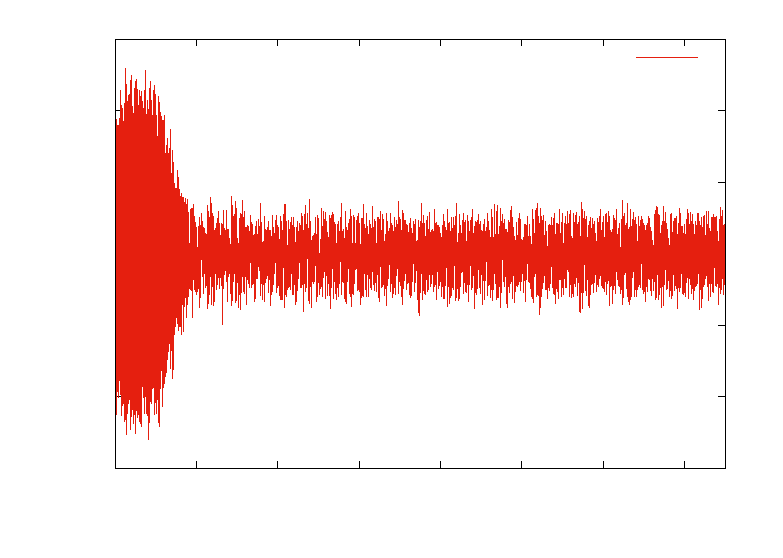
\includegraphics{plots/Echobeispeilsignal}}%
    \gplfronttext
  \end{picture}%
\endgroup

    \caption[]{ask: wie safed no data for differnet $\tau$, is it ok just to explain it that the amplitude will decrease and the maximum will be shifted to a different time? -> yes\\
    
    this is an example for a hahn echo with shimming value \SI{4.95}{x}.}
    \label{fig:Echobeispeilsignal}
\end{figure}
\begin{figure}[H]
    \centering
    % GNUPLOT: LaTeX picture with Postscript
\begingroup
  % Encoding inside the plot.  In the header of your document, this encoding
  % should to defined, e.g., by using
  % \usepackage[cp1252,<other encodings>]{inputenc}
  \inputencoding{cp1252}%
  \makeatletter
  \providecommand\color[2][]{%
    \GenericError{(gnuplot) \space\space\space\@spaces}{%
      Package color not loaded in conjunction with
      terminal option `colourtext'%
    }{See the gnuplot documentation for explanation.%
    }{Either use 'blacktext' in gnuplot or load the package
      color.sty in LaTeX.}%
    \renewcommand\color[2][]{}%
  }%
  \providecommand\includegraphics[2][]{%
    \GenericError{(gnuplot) \space\space\space\@spaces}{%
      Package graphicx or graphics not loaded%
    }{See the gnuplot documentation for explanation.%
    }{The gnuplot epslatex terminal needs graphicx.sty or graphics.sty.}%
    \renewcommand\includegraphics[2][]{}%
  }%
  \providecommand\rotatebox[2]{#2}%
  \@ifundefined{ifGPcolor}{%
    \newif\ifGPcolor
    \GPcolorfalse
  }{}%
  \@ifundefined{ifGPblacktext}{%
    \newif\ifGPblacktext
    \GPblacktexttrue
  }{}%
  % define a \g@addto@macro without @ in the name:
  \let\gplgaddtomacro\g@addto@macro
  % define empty templates for all commands taking text:
  \gdef\gplbacktext{}%
  \gdef\gplfronttext{}%
  \makeatother
  \ifGPblacktext
    % no textcolor at all
    \def\colorrgb#1{}%
    \def\colorgray#1{}%
  \else
    % gray or color?
    \ifGPcolor
      \def\colorrgb#1{\color[rgb]{#1}}%
      \def\colorgray#1{\color[gray]{#1}}%
      \expandafter\def\csname LTw\endcsname{\color{white}}%
      \expandafter\def\csname LTb\endcsname{\color{black}}%
      \expandafter\def\csname LTa\endcsname{\color{black}}%
      \expandafter\def\csname LT0\endcsname{\color[rgb]{1,0,0}}%
      \expandafter\def\csname LT1\endcsname{\color[rgb]{0,1,0}}%
      \expandafter\def\csname LT2\endcsname{\color[rgb]{0,0,1}}%
      \expandafter\def\csname LT3\endcsname{\color[rgb]{1,0,1}}%
      \expandafter\def\csname LT4\endcsname{\color[rgb]{0,1,1}}%
      \expandafter\def\csname LT5\endcsname{\color[rgb]{1,1,0}}%
      \expandafter\def\csname LT6\endcsname{\color[rgb]{0,0,0}}%
      \expandafter\def\csname LT7\endcsname{\color[rgb]{1,0.3,0}}%
      \expandafter\def\csname LT8\endcsname{\color[rgb]{0.5,0.5,0.5}}%
    \else
      % gray
      \def\colorrgb#1{\color{black}}%
      \def\colorgray#1{\color[gray]{#1}}%
      \expandafter\def\csname LTw\endcsname{\color{white}}%
      \expandafter\def\csname LTb\endcsname{\color{black}}%
      \expandafter\def\csname LTa\endcsname{\color{black}}%
      \expandafter\def\csname LT0\endcsname{\color{black}}%
      \expandafter\def\csname LT1\endcsname{\color{black}}%
      \expandafter\def\csname LT2\endcsname{\color{black}}%
      \expandafter\def\csname LT3\endcsname{\color{black}}%
      \expandafter\def\csname LT4\endcsname{\color{black}}%
      \expandafter\def\csname LT5\endcsname{\color{black}}%
      \expandafter\def\csname LT6\endcsname{\color{black}}%
      \expandafter\def\csname LT7\endcsname{\color{black}}%
      \expandafter\def\csname LT8\endcsname{\color{black}}%
    \fi
  \fi
    \setlength{\unitlength}{0.0500bp}%
    \ifx\gptboxheight\undefined%
      \newlength{\gptboxheight}%
      \newlength{\gptboxwidth}%
      \newsavebox{\gptboxtext}%
    \fi%
    \setlength{\fboxrule}{0.5pt}%
    \setlength{\fboxsep}{1pt}%
\begin{picture}(7200.00,5040.00)%
    \gplgaddtomacro\gplbacktext{%
      \csname LTb\endcsname%%
      \put(682,704){\makebox(0,0)[r]{\strut{}$0$}}%
      \put(682,1253){\makebox(0,0)[r]{\strut{}$2$}}%
      \put(682,1801){\makebox(0,0)[r]{\strut{}$4$}}%
      \put(682,2350){\makebox(0,0)[r]{\strut{}$6$}}%
      \put(682,2899){\makebox(0,0)[r]{\strut{}$8$}}%
      \put(682,3447){\makebox(0,0)[r]{\strut{}$10$}}%
      \put(682,3996){\makebox(0,0)[r]{\strut{}$12$}}%
      \put(682,4545){\makebox(0,0)[r]{\strut{}$14$}}%
      \put(814,484){\makebox(0,0){\strut{}$1800$}}%
      \put(1563,484){\makebox(0,0){\strut{}$1810$}}%
      \put(2311,484){\makebox(0,0){\strut{}$1820$}}%
      \put(3060,484){\makebox(0,0){\strut{}$1830$}}%
      \put(3809,484){\makebox(0,0){\strut{}$1840$}}%
      \put(4557,484){\makebox(0,0){\strut{}$1850$}}%
      \put(5306,484){\makebox(0,0){\strut{}$1860$}}%
      \put(6054,484){\makebox(0,0){\strut{}$1870$}}%
      \put(6803,484){\makebox(0,0){\strut{}$1880$}}%
    }%
    \gplgaddtomacro\gplfronttext{%
      \csname LTb\endcsname%%
      \put(209,2761){\rotatebox{-270}{\makebox(0,0){\strut{}FID amplitude}}}%
      \put(3808,154){\makebox(0,0){\strut{}Frequency in $\si{}{Hz}$}}%
      \csname LTb\endcsname%%
      \put(5816,4646){\makebox(0,0)[r]{\strut{}shimmin value $x = \si{0}{}}}%
      \csname LTb\endcsname%%
      \put(5816,4426){\makebox(0,0)[r]{\strut{}shimmin value $x = \si{4.95}{}}}%
    }%
    \gplbacktext
    \put(0,0){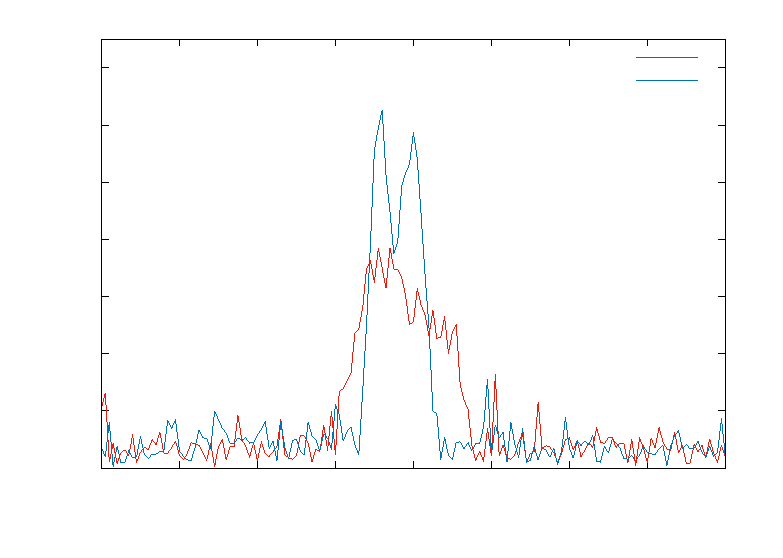
\includegraphics{plots/SpinEcho_4scans_ideal_Repetitiontime_0_shimming_150echo}}%
    \gplfronttext
  \end{picture}%
\endgroup

    \caption[]{ask: why are there different peaks a different shimming values?-> more frequency is sean (random) depends on position\newline
    which formula should we use to fit it? -> area under normalized spectrum should be the same; just discuss it -> narinder will send email\\
    
    for us: wieso signal schwächer-> mehr abweichung beim shimming (ursprünglich 10.11)-> abschwächung. integrale bei unterschiedlichen shimming; echo time 300ms bei beiden. }
    \label{fig:SpinEcho}
\end{figure}
We can measure T$_2$ when we don´t change the shimming values, because T$_2^*$ is dependent on a field inhomogeniousity. -> CPMG, Spin Hahn echo

% !TEX root = main.tex
\section{Multiple echo sequences}
\label{sec:Multipleechosequences}
Beside the \textit{Hahn} echo it is also possible to apply multiple \textit{Hahn} echos in one experimental measurement. This method is called \textit{Call-Purcell-Meiboom-Gill}-method (CPMG). Therefore the \SI{180}{\degree} pulse is applied every $2\tau$ and thus there accur many maximums in the signal every $2\tau$. The reason to use the CPMG method is that it is possible to measure the amplitude of two consecutiv maxima more often and therefore the measurement of T$_2$ is more precise. More about this will be discussed in the next chapter.\newline
To make the CPMG signals smoother in the time domain we do not use rectangular functions for the pulses, but smoothen them at the edge by a \textit{sine-bell-square} function. This is possible, due to the fact that it does not change the physical properties of our measurements, but will make them smoother.\newline
A main advantage of CMPG is that errors in the refocusing pulse can be vanished (minimize term of inhomogeneous magnetic field), by changing the phase between the B$_1$ excitation and the refocusing pulses. The program \textit{Prospa} profides a function called ''Constant 180 pulse phase''. This function keeps all the phases of the refocusing pulses equal. The second function \textit{Prospa} provides is ''Alternating 180 pulse phase''. This function compensates echo errors by alternating the refocusing pulses by \SI{180}{\degree}. In figure \ref{fig:180pulsephasedegree} it is visible what a change in the 180 pulse phase does to the signal. Unfortunately we only saved the signal vor 180 pulse phases of \SI{270}{\degree} and \SI{90}{\degree}. For those two values the signal does not change. That is also the reason why there is only one signal visible. The other one is just directly behind the other one and therefore not visible. If we would have saved a pulse phase of \SI{0}{\degree} or \SI{180}{\degree} the signal should change to a way faster decay and so the amplitude dies away really quickly.

\begin{figure}[H]
    \centering
    % GNUPLOT: LaTeX picture with Postscript
\begingroup
  % Encoding inside the plot.  In the header of your document, this encoding
  % should to defined, e.g., by using
  % \usepackage[cp1252,<other encodings>]{inputenc}
  \inputencoding{cp1252}%
  \makeatletter
  \providecommand\color[2][]{%
    \GenericError{(gnuplot) \space\space\space\@spaces}{%
      Package color not loaded in conjunction with
      terminal option `colourtext'%
    }{See the gnuplot documentation for explanation.%
    }{Either use 'blacktext' in gnuplot or load the package
      color.sty in LaTeX.}%
    \renewcommand\color[2][]{}%
  }%
  \providecommand\includegraphics[2][]{%
    \GenericError{(gnuplot) \space\space\space\@spaces}{%
      Package graphicx or graphics not loaded%
    }{See the gnuplot documentation for explanation.%
    }{The gnuplot epslatex terminal needs graphicx.sty or graphics.sty.}%
    \renewcommand\includegraphics[2][]{}%
  }%
  \providecommand\rotatebox[2]{#2}%
  \@ifundefined{ifGPcolor}{%
    \newif\ifGPcolor
    \GPcolorfalse
  }{}%
  \@ifundefined{ifGPblacktext}{%
    \newif\ifGPblacktext
    \GPblacktexttrue
  }{}%
  % define a \g@addto@macro without @ in the name:
  \let\gplgaddtomacro\g@addto@macro
  % define empty templates for all commands taking text:
  \gdef\gplbacktext{}%
  \gdef\gplfronttext{}%
  \makeatother
  \ifGPblacktext
    % no textcolor at all
    \def\colorrgb#1{}%
    \def\colorgray#1{}%
  \else
    % gray or color?
    \ifGPcolor
      \def\colorrgb#1{\color[rgb]{#1}}%
      \def\colorgray#1{\color[gray]{#1}}%
      \expandafter\def\csname LTw\endcsname{\color{white}}%
      \expandafter\def\csname LTb\endcsname{\color{black}}%
      \expandafter\def\csname LTa\endcsname{\color{black}}%
      \expandafter\def\csname LT0\endcsname{\color[rgb]{1,0,0}}%
      \expandafter\def\csname LT1\endcsname{\color[rgb]{0,1,0}}%
      \expandafter\def\csname LT2\endcsname{\color[rgb]{0,0,1}}%
      \expandafter\def\csname LT3\endcsname{\color[rgb]{1,0,1}}%
      \expandafter\def\csname LT4\endcsname{\color[rgb]{0,1,1}}%
      \expandafter\def\csname LT5\endcsname{\color[rgb]{1,1,0}}%
      \expandafter\def\csname LT6\endcsname{\color[rgb]{0,0,0}}%
      \expandafter\def\csname LT7\endcsname{\color[rgb]{1,0.3,0}}%
      \expandafter\def\csname LT8\endcsname{\color[rgb]{0.5,0.5,0.5}}%
    \else
      % gray
      \def\colorrgb#1{\color{black}}%
      \def\colorgray#1{\color[gray]{#1}}%
      \expandafter\def\csname LTw\endcsname{\color{white}}%
      \expandafter\def\csname LTb\endcsname{\color{black}}%
      \expandafter\def\csname LTa\endcsname{\color{black}}%
      \expandafter\def\csname LT0\endcsname{\color{black}}%
      \expandafter\def\csname LT1\endcsname{\color{black}}%
      \expandafter\def\csname LT2\endcsname{\color{black}}%
      \expandafter\def\csname LT3\endcsname{\color{black}}%
      \expandafter\def\csname LT4\endcsname{\color{black}}%
      \expandafter\def\csname LT5\endcsname{\color{black}}%
      \expandafter\def\csname LT6\endcsname{\color{black}}%
      \expandafter\def\csname LT7\endcsname{\color{black}}%
      \expandafter\def\csname LT8\endcsname{\color{black}}%
    \fi
  \fi
    \setlength{\unitlength}{0.0500bp}%
    \ifx\gptboxheight\undefined%
      \newlength{\gptboxheight}%
      \newlength{\gptboxwidth}%
      \newsavebox{\gptboxtext}%
    \fi%
    \setlength{\fboxrule}{0.5pt}%
    \setlength{\fboxsep}{1pt}%
\begin{picture}(7200.00,5040.00)%
    \gplgaddtomacro\gplbacktext{%
      \csname LTb\endcsname%%
      \put(814,704){\makebox(0,0)[r]{\strut{}$-60$}}%
      \put(814,1390){\makebox(0,0)[r]{\strut{}$-40$}}%
      \put(814,2076){\makebox(0,0)[r]{\strut{}$-20$}}%
      \put(814,2762){\makebox(0,0)[r]{\strut{}$0$}}%
      \put(814,3447){\makebox(0,0)[r]{\strut{}$20$}}%
      \put(814,4133){\makebox(0,0)[r]{\strut{}$40$}}%
      \put(814,4819){\makebox(0,0)[r]{\strut{}$60$}}%
      \put(946,484){\makebox(0,0){\strut{}$0$}}%
      \put(1783,484){\makebox(0,0){\strut{}$1000$}}%
      \put(2619,484){\makebox(0,0){\strut{}$2000$}}%
      \put(3456,484){\makebox(0,0){\strut{}$3000$}}%
      \put(4293,484){\makebox(0,0){\strut{}$4000$}}%
      \put(5130,484){\makebox(0,0){\strut{}$5000$}}%
      \put(5966,484){\makebox(0,0){\strut{}$6000$}}%
      \put(6803,484){\makebox(0,0){\strut{}$7000$}}%
    }%
    \gplgaddtomacro\gplfronttext{%
      \csname LTb\endcsname%%
      \put(209,2761){\rotatebox{-270}{\makebox(0,0){\strut{}Amplitude in $\si{\mu \volt}$}}}%
      \put(3874,154){\makebox(0,0){\strut{}Time in $\si{\second}$}}%
      \csname LTb\endcsname%%
      \put(5816,4646){\makebox(0,0)[r]{\strut{}180 pulse phase \SI{270}{\degree}}}%
      \csname LTb\endcsname%%
      \put(5816,4426){\makebox(0,0)[r]{\strut{}180 pulse phase \SI{90}{\degree}}}%
    }%
    \gplbacktext
    \put(0,0){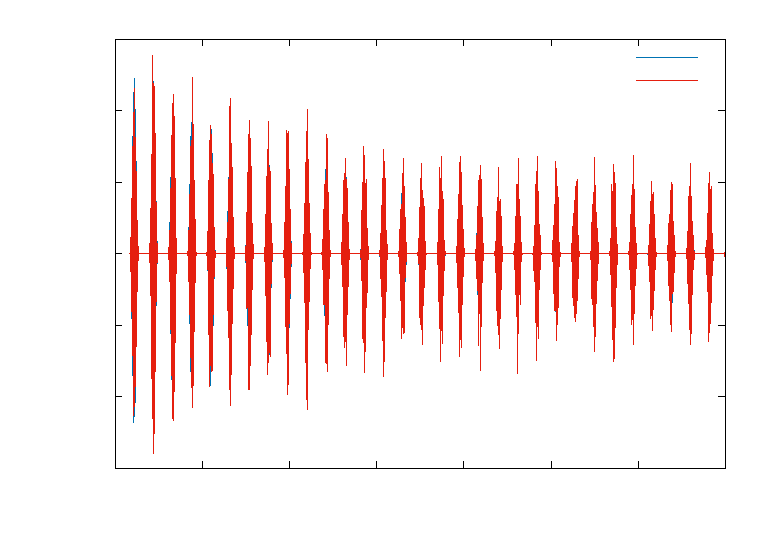
\includegraphics{plots/180pulsephasedegree}}%
    \gplfronttext
  \end{picture}%
\endgroup

    \caption[This figure shows the impact of the 180 pulse phase.]{This figure shows the impact of the 180 pulse phase. Unfortunately we only saved data for a 180 pulse phase of \SI{270}{\degree} and \SI{90}{\degree} and for those values it is correct that the signal does not change, but a signal for a 180 pulse phase of \SI{180}{\degree} would have shown a different signal.}
    \label{fig:180pulsephasedegree}
\end{figure}
 
% !TEX root = main.tex
\section{Transversal relaxation measurements}
\label{sec:Transversalrelaxationmeasurements}

\begin{figure}[H]
    \centering
    % GNUPLOT: LaTeX picture with Postscript
\begingroup
  % Encoding inside the plot.  In the header of your document, this encoding
  % should to defined, e.g., by using
  % \usepackage[cp1252,<other encodings>]{inputenc}
  \inputencoding{cp1252}%
  \makeatletter
  \providecommand\color[2][]{%
    \GenericError{(gnuplot) \space\space\space\@spaces}{%
      Package color not loaded in conjunction with
      terminal option `colourtext'%
    }{See the gnuplot documentation for explanation.%
    }{Either use 'blacktext' in gnuplot or load the package
      color.sty in LaTeX.}%
    \renewcommand\color[2][]{}%
  }%
  \providecommand\includegraphics[2][]{%
    \GenericError{(gnuplot) \space\space\space\@spaces}{%
      Package graphicx or graphics not loaded%
    }{See the gnuplot documentation for explanation.%
    }{The gnuplot epslatex terminal needs graphicx.sty or graphics.sty.}%
    \renewcommand\includegraphics[2][]{}%
  }%
  \providecommand\rotatebox[2]{#2}%
  \@ifundefined{ifGPcolor}{%
    \newif\ifGPcolor
    \GPcolorfalse
  }{}%
  \@ifundefined{ifGPblacktext}{%
    \newif\ifGPblacktext
    \GPblacktexttrue
  }{}%
  % define a \g@addto@macro without @ in the name:
  \let\gplgaddtomacro\g@addto@macro
  % define empty templates for all commands taking text:
  \gdef\gplbacktext{}%
  \gdef\gplfronttext{}%
  \makeatother
  \ifGPblacktext
    % no textcolor at all
    \def\colorrgb#1{}%
    \def\colorgray#1{}%
  \else
    % gray or color?
    \ifGPcolor
      \def\colorrgb#1{\color[rgb]{#1}}%
      \def\colorgray#1{\color[gray]{#1}}%
      \expandafter\def\csname LTw\endcsname{\color{white}}%
      \expandafter\def\csname LTb\endcsname{\color{black}}%
      \expandafter\def\csname LTa\endcsname{\color{black}}%
      \expandafter\def\csname LT0\endcsname{\color[rgb]{1,0,0}}%
      \expandafter\def\csname LT1\endcsname{\color[rgb]{0,1,0}}%
      \expandafter\def\csname LT2\endcsname{\color[rgb]{0,0,1}}%
      \expandafter\def\csname LT3\endcsname{\color[rgb]{1,0,1}}%
      \expandafter\def\csname LT4\endcsname{\color[rgb]{0,1,1}}%
      \expandafter\def\csname LT5\endcsname{\color[rgb]{1,1,0}}%
      \expandafter\def\csname LT6\endcsname{\color[rgb]{0,0,0}}%
      \expandafter\def\csname LT7\endcsname{\color[rgb]{1,0.3,0}}%
      \expandafter\def\csname LT8\endcsname{\color[rgb]{0.5,0.5,0.5}}%
    \else
      % gray
      \def\colorrgb#1{\color{black}}%
      \def\colorgray#1{\color[gray]{#1}}%
      \expandafter\def\csname LTw\endcsname{\color{white}}%
      \expandafter\def\csname LTb\endcsname{\color{black}}%
      \expandafter\def\csname LTa\endcsname{\color{black}}%
      \expandafter\def\csname LT0\endcsname{\color{black}}%
      \expandafter\def\csname LT1\endcsname{\color{black}}%
      \expandafter\def\csname LT2\endcsname{\color{black}}%
      \expandafter\def\csname LT3\endcsname{\color{black}}%
      \expandafter\def\csname LT4\endcsname{\color{black}}%
      \expandafter\def\csname LT5\endcsname{\color{black}}%
      \expandafter\def\csname LT6\endcsname{\color{black}}%
      \expandafter\def\csname LT7\endcsname{\color{black}}%
      \expandafter\def\csname LT8\endcsname{\color{black}}%
    \fi
  \fi
    \setlength{\unitlength}{0.0500bp}%
    \ifx\gptboxheight\undefined%
      \newlength{\gptboxheight}%
      \newlength{\gptboxwidth}%
      \newsavebox{\gptboxtext}%
    \fi%
    \setlength{\fboxrule}{0.5pt}%
    \setlength{\fboxsep}{1pt}%
\begin{picture}(7200.00,5040.00)%
    \gplgaddtomacro\gplbacktext{%
      \csname LTb\endcsname%%
      \put(814,704){\makebox(0,0)[r]{\strut{}$0$}}%
      \put(814,1527){\makebox(0,0)[r]{\strut{}$0.2$}}%
      \put(814,2350){\makebox(0,0)[r]{\strut{}$0.4$}}%
      \put(814,3173){\makebox(0,0)[r]{\strut{}$0.6$}}%
      \put(814,3996){\makebox(0,0)[r]{\strut{}$0.8$}}%
      \put(814,4819){\makebox(0,0)[r]{\strut{}$1$}}%
      \put(946,484){\makebox(0,0){\strut{}$0$}}%
      \put(1727,484){\makebox(0,0){\strut{}$1000$}}%
      \put(2508,484){\makebox(0,0){\strut{}$2000$}}%
      \put(3289,484){\makebox(0,0){\strut{}$3000$}}%
      \put(4070,484){\makebox(0,0){\strut{}$4000$}}%
      \put(4851,484){\makebox(0,0){\strut{}$5000$}}%
      \put(5632,484){\makebox(0,0){\strut{}$6000$}}%
      \put(6413,484){\makebox(0,0){\strut{}$7000$}}%
    }%
    \gplgaddtomacro\gplfronttext{%
      \csname LTb\endcsname%%
      \put(209,2761){\rotatebox{-270}{\makebox(0,0){\strut{}Attenuation $\frac{\text{E}}{\text{E}_0}$}}}%
      \put(3874,154){\makebox(0,0){\strut{}Time in $\si{\milli \second}$}}%
      \csname LTb\endcsname%%
      \put(5816,4646){\makebox(0,0)[r]{\strut{}measured data}}%
      \csname LTb\endcsname%%
      \put(5816,4426){\makebox(0,0)[r]{\strut{}attenuation Fit}}%
    }%
    \gplbacktext
    \put(0,0){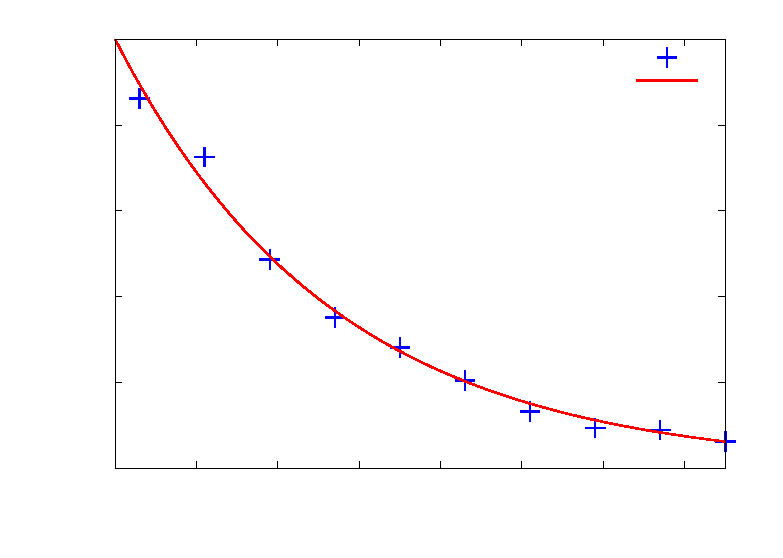
\includegraphics{plots/T2}}%
    \gplfronttext
  \end{picture}%
\endgroup

    \caption[]{ask: why are two peaks visible in the magnitude spectrum?\\
    normal FID-> T$_2$\newline
     $M(x)=M_0 \cdot exp(-x/T_2)$ with $T_2=\si{2691.06}{ms}$}
    \label{fig:T2}
\end{figure}

\begin{figure}[H]
    \centering
    % GNUPLOT: LaTeX picture with Postscript
\begingroup
  % Encoding inside the plot.  In the header of your document, this encoding
  % should to defined, e.g., by using
  % \usepackage[cp1252,<other encodings>]{inputenc}
  \inputencoding{cp1252}%
  \makeatletter
  \providecommand\color[2][]{%
    \GenericError{(gnuplot) \space\space\space\@spaces}{%
      Package color not loaded in conjunction with
      terminal option `colourtext'%
    }{See the gnuplot documentation for explanation.%
    }{Either use 'blacktext' in gnuplot or load the package
      color.sty in LaTeX.}%
    \renewcommand\color[2][]{}%
  }%
  \providecommand\includegraphics[2][]{%
    \GenericError{(gnuplot) \space\space\space\@spaces}{%
      Package graphicx or graphics not loaded%
    }{See the gnuplot documentation for explanation.%
    }{The gnuplot epslatex terminal needs graphicx.sty or graphics.sty.}%
    \renewcommand\includegraphics[2][]{}%
  }%
  \providecommand\rotatebox[2]{#2}%
  \@ifundefined{ifGPcolor}{%
    \newif\ifGPcolor
    \GPcolorfalse
  }{}%
  \@ifundefined{ifGPblacktext}{%
    \newif\ifGPblacktext
    \GPblacktexttrue
  }{}%
  % define a \g@addto@macro without @ in the name:
  \let\gplgaddtomacro\g@addto@macro
  % define empty templates for all commands taking text:
  \gdef\gplbacktext{}%
  \gdef\gplfronttext{}%
  \makeatother
  \ifGPblacktext
    % no textcolor at all
    \def\colorrgb#1{}%
    \def\colorgray#1{}%
  \else
    % gray or color?
    \ifGPcolor
      \def\colorrgb#1{\color[rgb]{#1}}%
      \def\colorgray#1{\color[gray]{#1}}%
      \expandafter\def\csname LTw\endcsname{\color{white}}%
      \expandafter\def\csname LTb\endcsname{\color{black}}%
      \expandafter\def\csname LTa\endcsname{\color{black}}%
      \expandafter\def\csname LT0\endcsname{\color[rgb]{1,0,0}}%
      \expandafter\def\csname LT1\endcsname{\color[rgb]{0,1,0}}%
      \expandafter\def\csname LT2\endcsname{\color[rgb]{0,0,1}}%
      \expandafter\def\csname LT3\endcsname{\color[rgb]{1,0,1}}%
      \expandafter\def\csname LT4\endcsname{\color[rgb]{0,1,1}}%
      \expandafter\def\csname LT5\endcsname{\color[rgb]{1,1,0}}%
      \expandafter\def\csname LT6\endcsname{\color[rgb]{0,0,0}}%
      \expandafter\def\csname LT7\endcsname{\color[rgb]{1,0.3,0}}%
      \expandafter\def\csname LT8\endcsname{\color[rgb]{0.5,0.5,0.5}}%
    \else
      % gray
      \def\colorrgb#1{\color{black}}%
      \def\colorgray#1{\color[gray]{#1}}%
      \expandafter\def\csname LTw\endcsname{\color{white}}%
      \expandafter\def\csname LTb\endcsname{\color{black}}%
      \expandafter\def\csname LTa\endcsname{\color{black}}%
      \expandafter\def\csname LT0\endcsname{\color{black}}%
      \expandafter\def\csname LT1\endcsname{\color{black}}%
      \expandafter\def\csname LT2\endcsname{\color{black}}%
      \expandafter\def\csname LT3\endcsname{\color{black}}%
      \expandafter\def\csname LT4\endcsname{\color{black}}%
      \expandafter\def\csname LT5\endcsname{\color{black}}%
      \expandafter\def\csname LT6\endcsname{\color{black}}%
      \expandafter\def\csname LT7\endcsname{\color{black}}%
      \expandafter\def\csname LT8\endcsname{\color{black}}%
    \fi
  \fi
    \setlength{\unitlength}{0.0500bp}%
    \ifx\gptboxheight\undefined%
      \newlength{\gptboxheight}%
      \newlength{\gptboxwidth}%
      \newsavebox{\gptboxtext}%
    \fi%
    \setlength{\fboxrule}{0.5pt}%
    \setlength{\fboxsep}{1pt}%
\begin{picture}(7200.00,5040.00)%
    \gplgaddtomacro\gplbacktext{%
      \csname LTb\endcsname%%
      \put(814,704){\makebox(0,0)[r]{\strut{}$0$}}%
      \put(814,1527){\makebox(0,0)[r]{\strut{}$0.2$}}%
      \put(814,2350){\makebox(0,0)[r]{\strut{}$0.4$}}%
      \put(814,3173){\makebox(0,0)[r]{\strut{}$0.6$}}%
      \put(814,3996){\makebox(0,0)[r]{\strut{}$0.8$}}%
      \put(814,4819){\makebox(0,0)[r]{\strut{}$1$}}%
      \put(1754,484){\makebox(0,0){\strut{}$1000$}}%
      \put(2764,484){\makebox(0,0){\strut{}$2000$}}%
      \put(3774,484){\makebox(0,0){\strut{}$3000$}}%
      \put(4783,484){\makebox(0,0){\strut{}$4000$}}%
      \put(5793,484){\makebox(0,0){\strut{}$5000$}}%
      \put(6803,484){\makebox(0,0){\strut{}$6000$}}%
    }%
    \gplgaddtomacro\gplfronttext{%
      \csname LTb\endcsname%%
      \put(209,2761){\rotatebox{-270}{\makebox(0,0){\strut{}Amplitude $\frac{\text{E}}{\text{E}_0}$}}}%
      \put(3874,154){\makebox(0,0){\strut{}Time in $\si{\milli \second}$}}%
      \csname LTb\endcsname%%
      \put(5816,4646){\makebox(0,0)[r]{\strut{}measured data}}%
      \csname LTb\endcsname%%
      \put(5816,4426){\makebox(0,0)[r]{\strut{}attenuation-Fit}}%
    }%
    \gplbacktext
    \put(0,0){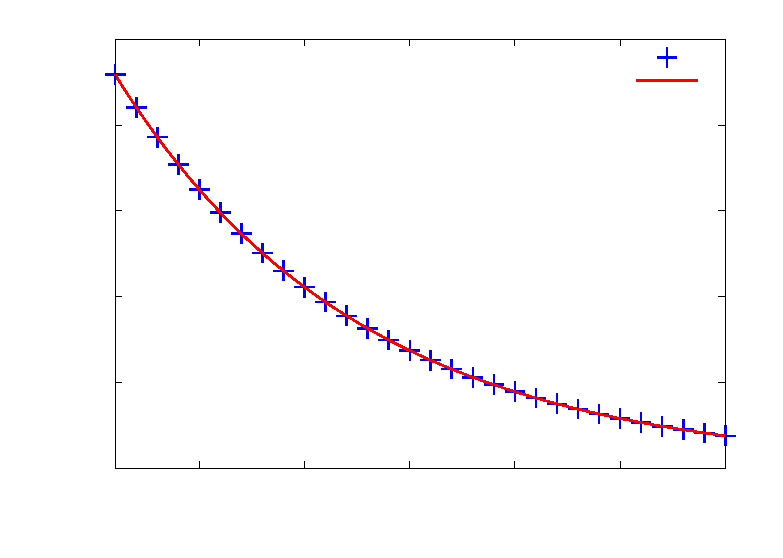
\includegraphics{plots/CPMG045shimming}}%
    \gplfronttext
  \end{picture}%
\endgroup

    \caption[]{This is an CPMG with changeed values in the shimming; shimming value \SI{0.45}{x} -> T$_2^*$.\newline
    Good to see that the T$_2^*$ is here shorter than in the previous picture, due to inhomogeniousity of the magnetic field.\\
    $M(x)=M_0 \cdot exp(-x/T_2)$ with $T_2=\SI{2317.76}{\milli \second}$}
    \label{fig:CPMG}
\end{figure}

\selectlanguage{ngerman}
% !TEX root = main.tex
\section{Fourietrafo der Messungen mit unterschieldicheer Polarisationszeit}
\begin{figure}[H]
    \centering
    % !TEX root = main.tex
\section{Fourietrafo der Messungen mit unterschieldicheer Polarisationszeit}
\begin{figure}[H]
    \centering
    % !TEX root = main.tex
\section{Fourietrafo der Messungen mit unterschieldicheer Polarisationszeit}
\begin{figure}[H]
    \centering
    \input{plots/Polarisationszeit.tex}
    \caption{Amplitude in abhängigkeit von zwei verschiedenen Piolarisatiosnzeiten}
\end{figure}
    \caption{Amplitude in abhängigkeit von zwei verschiedenen Piolarisatiosnzeiten}
\end{figure}
    \caption{Amplitude in abhängigkeit von zwei verschiedenen Piolarisatiosnzeiten}
\end{figure}
% !TEX root = main.tex
\section{T1 und T2 Relaxationszeit für Wasser und mit Zusatzmitteln}
\begin{figure}[H]
    \centering
    % GNUPLOT: LaTeX picture with Postscript
\begingroup
  % Encoding inside the plot.  In the header of your document, this encoding
  % should to defined, e.g., by using
  % \usepackage[cp1252,<other encodings>]{inputenc}
  \inputencoding{cp1252}%
  \makeatletter
  \providecommand\color[2][]{%
    \GenericError{(gnuplot) \space\space\space\@spaces}{%
      Package color not loaded in conjunction with
      terminal option `colourtext'%
    }{See the gnuplot documentation for explanation.%
    }{Either use 'blacktext' in gnuplot or load the package
      color.sty in LaTeX.}%
    \renewcommand\color[2][]{}%
  }%
  \providecommand\includegraphics[2][]{%
    \GenericError{(gnuplot) \space\space\space\@spaces}{%
      Package graphicx or graphics not loaded%
    }{See the gnuplot documentation for explanation.%
    }{The gnuplot epslatex terminal needs graphicx.sty or graphics.sty.}%
    \renewcommand\includegraphics[2][]{}%
  }%
  \providecommand\rotatebox[2]{#2}%
  \@ifundefined{ifGPcolor}{%
    \newif\ifGPcolor
    \GPcolorfalse
  }{}%
  \@ifundefined{ifGPblacktext}{%
    \newif\ifGPblacktext
    \GPblacktexttrue
  }{}%
  % define a \g@addto@macro without @ in the name:
  \let\gplgaddtomacro\g@addto@macro
  % define empty templates for all commands taking text:
  \gdef\gplbacktext{}%
  \gdef\gplfronttext{}%
  \makeatother
  \ifGPblacktext
    % no textcolor at all
    \def\colorrgb#1{}%
    \def\colorgray#1{}%
  \else
    % gray or color?
    \ifGPcolor
      \def\colorrgb#1{\color[rgb]{#1}}%
      \def\colorgray#1{\color[gray]{#1}}%
      \expandafter\def\csname LTw\endcsname{\color{white}}%
      \expandafter\def\csname LTb\endcsname{\color{black}}%
      \expandafter\def\csname LTa\endcsname{\color{black}}%
      \expandafter\def\csname LT0\endcsname{\color[rgb]{1,0,0}}%
      \expandafter\def\csname LT1\endcsname{\color[rgb]{0,1,0}}%
      \expandafter\def\csname LT2\endcsname{\color[rgb]{0,0,1}}%
      \expandafter\def\csname LT3\endcsname{\color[rgb]{1,0,1}}%
      \expandafter\def\csname LT4\endcsname{\color[rgb]{0,1,1}}%
      \expandafter\def\csname LT5\endcsname{\color[rgb]{1,1,0}}%
      \expandafter\def\csname LT6\endcsname{\color[rgb]{0,0,0}}%
      \expandafter\def\csname LT7\endcsname{\color[rgb]{1,0.3,0}}%
      \expandafter\def\csname LT8\endcsname{\color[rgb]{0.5,0.5,0.5}}%
    \else
      % gray
      \def\colorrgb#1{\color{black}}%
      \def\colorgray#1{\color[gray]{#1}}%
      \expandafter\def\csname LTw\endcsname{\color{white}}%
      \expandafter\def\csname LTb\endcsname{\color{black}}%
      \expandafter\def\csname LTa\endcsname{\color{black}}%
      \expandafter\def\csname LT0\endcsname{\color{black}}%
      \expandafter\def\csname LT1\endcsname{\color{black}}%
      \expandafter\def\csname LT2\endcsname{\color{black}}%
      \expandafter\def\csname LT3\endcsname{\color{black}}%
      \expandafter\def\csname LT4\endcsname{\color{black}}%
      \expandafter\def\csname LT5\endcsname{\color{black}}%
      \expandafter\def\csname LT6\endcsname{\color{black}}%
      \expandafter\def\csname LT7\endcsname{\color{black}}%
      \expandafter\def\csname LT8\endcsname{\color{black}}%
    \fi
  \fi
    \setlength{\unitlength}{0.0500bp}%
    \ifx\gptboxheight\undefined%
      \newlength{\gptboxheight}%
      \newlength{\gptboxwidth}%
      \newsavebox{\gptboxtext}%
    \fi%
    \setlength{\fboxrule}{0.5pt}%
    \setlength{\fboxsep}{1pt}%
\begin{picture}(7200.00,5040.00)%
    \gplgaddtomacro\gplbacktext{%
      \csname LTb\endcsname%%
      \put(814,704){\makebox(0,0)[r]{\strut{}$0$}}%
      \put(814,1527){\makebox(0,0)[r]{\strut{}$0.2$}}%
      \put(814,2350){\makebox(0,0)[r]{\strut{}$0.4$}}%
      \put(814,3173){\makebox(0,0)[r]{\strut{}$0.6$}}%
      \put(814,3996){\makebox(0,0)[r]{\strut{}$0.8$}}%
      \put(814,4819){\makebox(0,0)[r]{\strut{}$1$}}%
      \put(946,484){\makebox(0,0){\strut{}$0$}}%
      \put(1660,484){\makebox(0,0){\strut{}$500$}}%
      \put(2375,484){\makebox(0,0){\strut{}$1000$}}%
      \put(3089,484){\makebox(0,0){\strut{}$1500$}}%
      \put(3803,484){\makebox(0,0){\strut{}$2000$}}%
      \put(4517,484){\makebox(0,0){\strut{}$2500$}}%
      \put(5232,484){\makebox(0,0){\strut{}$3000$}}%
      \put(5946,484){\makebox(0,0){\strut{}$3500$}}%
      \put(6660,484){\makebox(0,0){\strut{}$4000$}}%
    }%
    \gplgaddtomacro\gplfronttext{%
      \csname LTb\endcsname%%
      \put(308,2761){\rotatebox{-270}{\makebox(0,0){\strut{}D\"ampfung $\frac{\text{E}}{\text{E}_0}$}}}%
      \put(3874,154){\makebox(0,0){\strut{}Zeit zwischen den Pulsen $t$ in $\si{\milli \second}$}}%
      \csname LTb\endcsname%%
      \put(5860,4606){\makebox(0,0)[r]{\strut{}gemessene Datenpunkte f\"ur Wasser}}%
      \csname LTb\endcsname%%
      \put(5860,4386){\makebox(0,0)[r]{\strut{}exponentieller Fit}}%
    }%
    \gplbacktext
    \put(0,0){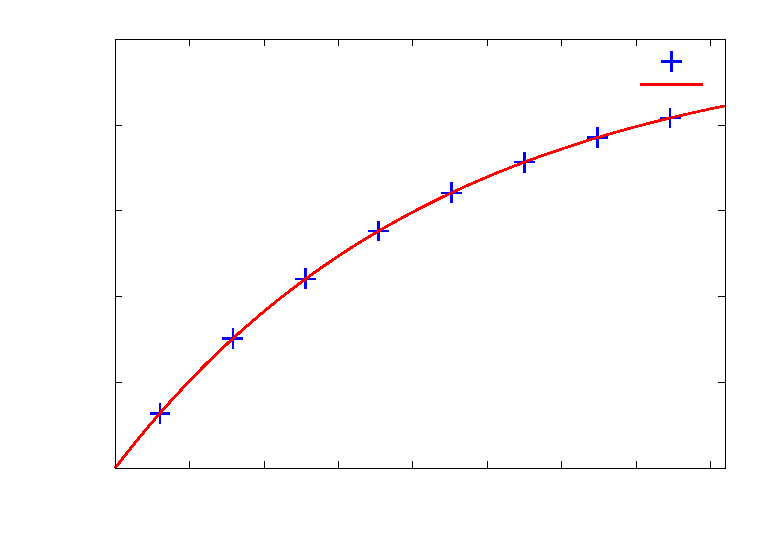
\includegraphics{plots/T1Wasser}}%
    \gplfronttext
  \end{picture}%
\endgroup

    \caption{T1 Messung von Wasser}
\end{figure}

\begin{figure}[H]
    \centering
    % GNUPLOT: LaTeX picture with Postscript
\begingroup
  % Encoding inside the plot.  In the header of your document, this encoding
  % should to defined, e.g., by using
  % \usepackage[cp1252,<other encodings>]{inputenc}
  \inputencoding{cp1252}%
  \makeatletter
  \providecommand\color[2][]{%
    \GenericError{(gnuplot) \space\space\space\@spaces}{%
      Package color not loaded in conjunction with
      terminal option `colourtext'%
    }{See the gnuplot documentation for explanation.%
    }{Either use 'blacktext' in gnuplot or load the package
      color.sty in LaTeX.}%
    \renewcommand\color[2][]{}%
  }%
  \providecommand\includegraphics[2][]{%
    \GenericError{(gnuplot) \space\space\space\@spaces}{%
      Package graphicx or graphics not loaded%
    }{See the gnuplot documentation for explanation.%
    }{The gnuplot epslatex terminal needs graphicx.sty or graphics.sty.}%
    \renewcommand\includegraphics[2][]{}%
  }%
  \providecommand\rotatebox[2]{#2}%
  \@ifundefined{ifGPcolor}{%
    \newif\ifGPcolor
    \GPcolorfalse
  }{}%
  \@ifundefined{ifGPblacktext}{%
    \newif\ifGPblacktext
    \GPblacktexttrue
  }{}%
  % define a \g@addto@macro without @ in the name:
  \let\gplgaddtomacro\g@addto@macro
  % define empty templates for all commands taking text:
  \gdef\gplbacktext{}%
  \gdef\gplfronttext{}%
  \makeatother
  \ifGPblacktext
    % no textcolor at all
    \def\colorrgb#1{}%
    \def\colorgray#1{}%
  \else
    % gray or color?
    \ifGPcolor
      \def\colorrgb#1{\color[rgb]{#1}}%
      \def\colorgray#1{\color[gray]{#1}}%
      \expandafter\def\csname LTw\endcsname{\color{white}}%
      \expandafter\def\csname LTb\endcsname{\color{black}}%
      \expandafter\def\csname LTa\endcsname{\color{black}}%
      \expandafter\def\csname LT0\endcsname{\color[rgb]{1,0,0}}%
      \expandafter\def\csname LT1\endcsname{\color[rgb]{0,1,0}}%
      \expandafter\def\csname LT2\endcsname{\color[rgb]{0,0,1}}%
      \expandafter\def\csname LT3\endcsname{\color[rgb]{1,0,1}}%
      \expandafter\def\csname LT4\endcsname{\color[rgb]{0,1,1}}%
      \expandafter\def\csname LT5\endcsname{\color[rgb]{1,1,0}}%
      \expandafter\def\csname LT6\endcsname{\color[rgb]{0,0,0}}%
      \expandafter\def\csname LT7\endcsname{\color[rgb]{1,0.3,0}}%
      \expandafter\def\csname LT8\endcsname{\color[rgb]{0.5,0.5,0.5}}%
    \else
      % gray
      \def\colorrgb#1{\color{black}}%
      \def\colorgray#1{\color[gray]{#1}}%
      \expandafter\def\csname LTw\endcsname{\color{white}}%
      \expandafter\def\csname LTb\endcsname{\color{black}}%
      \expandafter\def\csname LTa\endcsname{\color{black}}%
      \expandafter\def\csname LT0\endcsname{\color{black}}%
      \expandafter\def\csname LT1\endcsname{\color{black}}%
      \expandafter\def\csname LT2\endcsname{\color{black}}%
      \expandafter\def\csname LT3\endcsname{\color{black}}%
      \expandafter\def\csname LT4\endcsname{\color{black}}%
      \expandafter\def\csname LT5\endcsname{\color{black}}%
      \expandafter\def\csname LT6\endcsname{\color{black}}%
      \expandafter\def\csname LT7\endcsname{\color{black}}%
      \expandafter\def\csname LT8\endcsname{\color{black}}%
    \fi
  \fi
    \setlength{\unitlength}{0.0500bp}%
    \ifx\gptboxheight\undefined%
      \newlength{\gptboxheight}%
      \newlength{\gptboxwidth}%
      \newsavebox{\gptboxtext}%
    \fi%
    \setlength{\fboxrule}{0.5pt}%
    \setlength{\fboxsep}{1pt}%
\begin{picture}(7200.00,5040.00)%
    \gplgaddtomacro\gplbacktext{%
      \csname LTb\endcsname%%
      \put(814,704){\makebox(0,0)[r]{\strut{}$0$}}%
      \put(814,1527){\makebox(0,0)[r]{\strut{}$0.2$}}%
      \put(814,2350){\makebox(0,0)[r]{\strut{}$0.4$}}%
      \put(814,3173){\makebox(0,0)[r]{\strut{}$0.6$}}%
      \put(814,3996){\makebox(0,0)[r]{\strut{}$0.8$}}%
      \put(814,4819){\makebox(0,0)[r]{\strut{}$1$}}%
      \put(946,484){\makebox(0,0){\strut{}$0$}}%
      \put(1922,484){\makebox(0,0){\strut{}$1000$}}%
      \put(2898,484){\makebox(0,0){\strut{}$2000$}}%
      \put(3875,484){\makebox(0,0){\strut{}$3000$}}%
      \put(4851,484){\makebox(0,0){\strut{}$4000$}}%
      \put(5827,484){\makebox(0,0){\strut{}$5000$}}%
      \put(6803,484){\makebox(0,0){\strut{}$6000$}}%
    }%
    \gplgaddtomacro\gplfronttext{%
      \csname LTb\endcsname%%
      \put(308,2761){\rotatebox{-270}{\makebox(0,0){\strut{}Dämpfung $\frac{\text{E}}{\text{E}_0}$}}}%
      \put(3874,154){\makebox(0,0){\strut{}Zeit in $\si{\milli \second}$}}%
      \csname LTb\endcsname%%
      \put(5860,4606){\makebox(0,0)[r]{\strut{}gemessene Datenpunkte für Wasser}}%
      \csname LTb\endcsname%%
      \put(5860,4386){\makebox(0,0)[r]{\strut{}Dämpfungsfit Fit}}%
    }%
    \gplbacktext
    \put(0,0){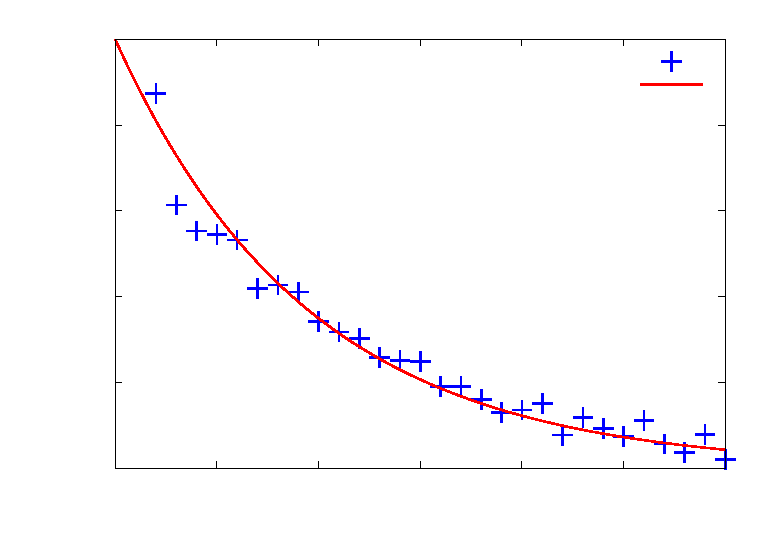
\includegraphics{plots/T2Wasser}}%
    \gplfronttext
  \end{picture}%
\endgroup

    \caption{T2 Messung von Wasser}
\end{figure}

% \begin{figure}[H]
%     \centering
%     % GNUPLOT: LaTeX picture with Postscript
\begingroup
  % Encoding inside the plot.  In the header of your document, this encoding
  % should to defined, e.g., by using
  % \usepackage[cp1252,<other encodings>]{inputenc}
  \inputencoding{cp1252}%
  \makeatletter
  \providecommand\color[2][]{%
    \GenericError{(gnuplot) \space\space\space\@spaces}{%
      Package color not loaded in conjunction with
      terminal option `colourtext'%
    }{See the gnuplot documentation for explanation.%
    }{Either use 'blacktext' in gnuplot or load the package
      color.sty in LaTeX.}%
    \renewcommand\color[2][]{}%
  }%
  \providecommand\includegraphics[2][]{%
    \GenericError{(gnuplot) \space\space\space\@spaces}{%
      Package graphicx or graphics not loaded%
    }{See the gnuplot documentation for explanation.%
    }{The gnuplot epslatex terminal needs graphicx.sty or graphics.sty.}%
    \renewcommand\includegraphics[2][]{}%
  }%
  \providecommand\rotatebox[2]{#2}%
  \@ifundefined{ifGPcolor}{%
    \newif\ifGPcolor
    \GPcolorfalse
  }{}%
  \@ifundefined{ifGPblacktext}{%
    \newif\ifGPblacktext
    \GPblacktexttrue
  }{}%
  % define a \g@addto@macro without @ in the name:
  \let\gplgaddtomacro\g@addto@macro
  % define empty templates for all commands taking text:
  \gdef\gplbacktext{}%
  \gdef\gplfronttext{}%
  \makeatother
  \ifGPblacktext
    % no textcolor at all
    \def\colorrgb#1{}%
    \def\colorgray#1{}%
  \else
    % gray or color?
    \ifGPcolor
      \def\colorrgb#1{\color[rgb]{#1}}%
      \def\colorgray#1{\color[gray]{#1}}%
      \expandafter\def\csname LTw\endcsname{\color{white}}%
      \expandafter\def\csname LTb\endcsname{\color{black}}%
      \expandafter\def\csname LTa\endcsname{\color{black}}%
      \expandafter\def\csname LT0\endcsname{\color[rgb]{1,0,0}}%
      \expandafter\def\csname LT1\endcsname{\color[rgb]{0,1,0}}%
      \expandafter\def\csname LT2\endcsname{\color[rgb]{0,0,1}}%
      \expandafter\def\csname LT3\endcsname{\color[rgb]{1,0,1}}%
      \expandafter\def\csname LT4\endcsname{\color[rgb]{0,1,1}}%
      \expandafter\def\csname LT5\endcsname{\color[rgb]{1,1,0}}%
      \expandafter\def\csname LT6\endcsname{\color[rgb]{0,0,0}}%
      \expandafter\def\csname LT7\endcsname{\color[rgb]{1,0.3,0}}%
      \expandafter\def\csname LT8\endcsname{\color[rgb]{0.5,0.5,0.5}}%
    \else
      % gray
      \def\colorrgb#1{\color{black}}%
      \def\colorgray#1{\color[gray]{#1}}%
      \expandafter\def\csname LTw\endcsname{\color{white}}%
      \expandafter\def\csname LTb\endcsname{\color{black}}%
      \expandafter\def\csname LTa\endcsname{\color{black}}%
      \expandafter\def\csname LT0\endcsname{\color{black}}%
      \expandafter\def\csname LT1\endcsname{\color{black}}%
      \expandafter\def\csname LT2\endcsname{\color{black}}%
      \expandafter\def\csname LT3\endcsname{\color{black}}%
      \expandafter\def\csname LT4\endcsname{\color{black}}%
      \expandafter\def\csname LT5\endcsname{\color{black}}%
      \expandafter\def\csname LT6\endcsname{\color{black}}%
      \expandafter\def\csname LT7\endcsname{\color{black}}%
      \expandafter\def\csname LT8\endcsname{\color{black}}%
    \fi
  \fi
    \setlength{\unitlength}{0.0500bp}%
    \ifx\gptboxheight\undefined%
      \newlength{\gptboxheight}%
      \newlength{\gptboxwidth}%
      \newsavebox{\gptboxtext}%
    \fi%
    \setlength{\fboxrule}{0.5pt}%
    \setlength{\fboxsep}{1pt}%
\begin{picture}(7200.00,5040.00)%
    \gplgaddtomacro\gplbacktext{%
      \csname LTb\endcsname%%
      \put(814,704){\makebox(0,0)[r]{\strut{}$0$}}%
      \put(814,1527){\makebox(0,0)[r]{\strut{}$0.2$}}%
      \put(814,2350){\makebox(0,0)[r]{\strut{}$0.4$}}%
      \put(814,3173){\makebox(0,0)[r]{\strut{}$0.6$}}%
      \put(814,3996){\makebox(0,0)[r]{\strut{}$0.8$}}%
      \put(814,4819){\makebox(0,0)[r]{\strut{}$1$}}%
      \put(946,484){\makebox(0,0){\strut{}$0$}}%
      \put(1563,484){\makebox(0,0){\strut{}$500$}}%
      \put(2179,484){\makebox(0,0){\strut{}$1000$}}%
      \put(2796,484){\makebox(0,0){\strut{}$1500$}}%
      \put(3412,484){\makebox(0,0){\strut{}$2000$}}%
      \put(4029,484){\makebox(0,0){\strut{}$2500$}}%
      \put(4645,484){\makebox(0,0){\strut{}$3000$}}%
      \put(5262,484){\makebox(0,0){\strut{}$3500$}}%
      \put(5878,484){\makebox(0,0){\strut{}$4000$}}%
      \put(6495,484){\makebox(0,0){\strut{}$4500$}}%
    }%
    \gplgaddtomacro\gplfronttext{%
      \csname LTb\endcsname%%
      \put(308,2761){\rotatebox{-270}{\makebox(0,0){\strut{}D\"ampfung $\frac{\text{E}}{\text{E}_0}$}}}%
      \put(3874,154){\makebox(0,0){\strut{}Zeit zwischen den Pulsen $t$ in $\si{\milli \second}$}}%
      \csname LTb\endcsname%%
      \put(5860,4606){\makebox(0,0)[r]{\strut{}gemessene Datenpunkte f\"ur $Cu^{2+} \SI{250}{\micro\mole}$}}%
      \csname LTb\endcsname%%
      \put(5860,4386){\makebox(0,0)[r]{\strut{}exponentieller Fit}}%
    }%
    \gplbacktext
    \put(0,0){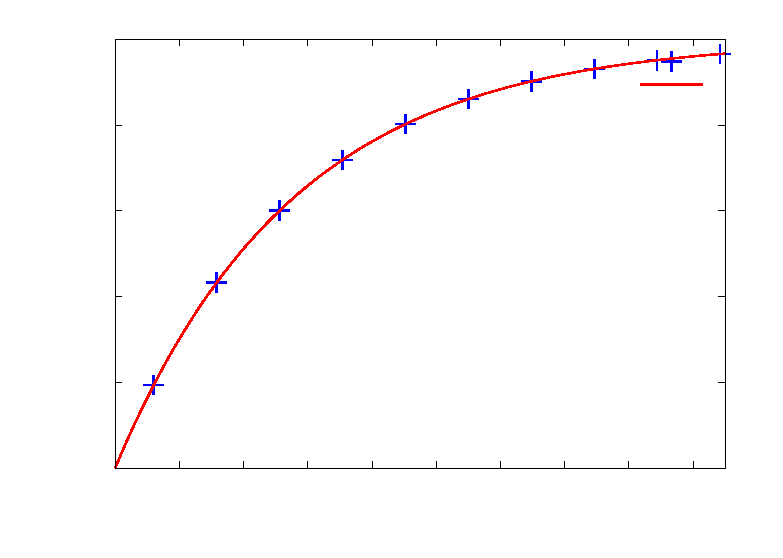
\includegraphics{plots/T1Kupfer250}}%
    \gplfronttext
  \end{picture}%
\endgroup

%     \caption{T1 Messung Kupfer $Cu^{2+} \SI{250}{\micro\mole}$}
% \end{figure}

% \begin{figure}[H]
%     \centering
%     % GNUPLOT: LaTeX picture with Postscript
\begingroup
  % Encoding inside the plot.  In the header of your document, this encoding
  % should to defined, e.g., by using
  % \usepackage[cp1252,<other encodings>]{inputenc}
  \inputencoding{cp1252}%
  \makeatletter
  \providecommand\color[2][]{%
    \GenericError{(gnuplot) \space\space\space\@spaces}{%
      Package color not loaded in conjunction with
      terminal option `colourtext'%
    }{See the gnuplot documentation for explanation.%
    }{Either use 'blacktext' in gnuplot or load the package
      color.sty in LaTeX.}%
    \renewcommand\color[2][]{}%
  }%
  \providecommand\includegraphics[2][]{%
    \GenericError{(gnuplot) \space\space\space\@spaces}{%
      Package graphicx or graphics not loaded%
    }{See the gnuplot documentation for explanation.%
    }{The gnuplot epslatex terminal needs graphicx.sty or graphics.sty.}%
    \renewcommand\includegraphics[2][]{}%
  }%
  \providecommand\rotatebox[2]{#2}%
  \@ifundefined{ifGPcolor}{%
    \newif\ifGPcolor
    \GPcolorfalse
  }{}%
  \@ifundefined{ifGPblacktext}{%
    \newif\ifGPblacktext
    \GPblacktexttrue
  }{}%
  % define a \g@addto@macro without @ in the name:
  \let\gplgaddtomacro\g@addto@macro
  % define empty templates for all commands taking text:
  \gdef\gplbacktext{}%
  \gdef\gplfronttext{}%
  \makeatother
  \ifGPblacktext
    % no textcolor at all
    \def\colorrgb#1{}%
    \def\colorgray#1{}%
  \else
    % gray or color?
    \ifGPcolor
      \def\colorrgb#1{\color[rgb]{#1}}%
      \def\colorgray#1{\color[gray]{#1}}%
      \expandafter\def\csname LTw\endcsname{\color{white}}%
      \expandafter\def\csname LTb\endcsname{\color{black}}%
      \expandafter\def\csname LTa\endcsname{\color{black}}%
      \expandafter\def\csname LT0\endcsname{\color[rgb]{1,0,0}}%
      \expandafter\def\csname LT1\endcsname{\color[rgb]{0,1,0}}%
      \expandafter\def\csname LT2\endcsname{\color[rgb]{0,0,1}}%
      \expandafter\def\csname LT3\endcsname{\color[rgb]{1,0,1}}%
      \expandafter\def\csname LT4\endcsname{\color[rgb]{0,1,1}}%
      \expandafter\def\csname LT5\endcsname{\color[rgb]{1,1,0}}%
      \expandafter\def\csname LT6\endcsname{\color[rgb]{0,0,0}}%
      \expandafter\def\csname LT7\endcsname{\color[rgb]{1,0.3,0}}%
      \expandafter\def\csname LT8\endcsname{\color[rgb]{0.5,0.5,0.5}}%
    \else
      % gray
      \def\colorrgb#1{\color{black}}%
      \def\colorgray#1{\color[gray]{#1}}%
      \expandafter\def\csname LTw\endcsname{\color{white}}%
      \expandafter\def\csname LTb\endcsname{\color{black}}%
      \expandafter\def\csname LTa\endcsname{\color{black}}%
      \expandafter\def\csname LT0\endcsname{\color{black}}%
      \expandafter\def\csname LT1\endcsname{\color{black}}%
      \expandafter\def\csname LT2\endcsname{\color{black}}%
      \expandafter\def\csname LT3\endcsname{\color{black}}%
      \expandafter\def\csname LT4\endcsname{\color{black}}%
      \expandafter\def\csname LT5\endcsname{\color{black}}%
      \expandafter\def\csname LT6\endcsname{\color{black}}%
      \expandafter\def\csname LT7\endcsname{\color{black}}%
      \expandafter\def\csname LT8\endcsname{\color{black}}%
    \fi
  \fi
    \setlength{\unitlength}{0.0500bp}%
    \ifx\gptboxheight\undefined%
      \newlength{\gptboxheight}%
      \newlength{\gptboxwidth}%
      \newsavebox{\gptboxtext}%
    \fi%
    \setlength{\fboxrule}{0.5pt}%
    \setlength{\fboxsep}{1pt}%
\begin{picture}(7200.00,5040.00)%
    \gplgaddtomacro\gplbacktext{%
      \csname LTb\endcsname%%
      \put(814,704){\makebox(0,0)[r]{\strut{}$0$}}%
      \put(814,1527){\makebox(0,0)[r]{\strut{}$0.2$}}%
      \put(814,2350){\makebox(0,0)[r]{\strut{}$0.4$}}%
      \put(814,3173){\makebox(0,0)[r]{\strut{}$0.6$}}%
      \put(814,3996){\makebox(0,0)[r]{\strut{}$0.8$}}%
      \put(814,4819){\makebox(0,0)[r]{\strut{}$1$}}%
      \put(946,484){\makebox(0,0){\strut{}$0$}}%
      \put(1922,484){\makebox(0,0){\strut{}$1000$}}%
      \put(2898,484){\makebox(0,0){\strut{}$2000$}}%
      \put(3875,484){\makebox(0,0){\strut{}$3000$}}%
      \put(4851,484){\makebox(0,0){\strut{}$4000$}}%
      \put(5827,484){\makebox(0,0){\strut{}$5000$}}%
      \put(6803,484){\makebox(0,0){\strut{}$6000$}}%
    }%
    \gplgaddtomacro\gplfronttext{%
      \csname LTb\endcsname%%
      \put(308,2761){\rotatebox{-270}{\makebox(0,0){\strut{}Dämpfung $\frac{\text{E}}{\text{E}_0}$}}}%
      \put(3874,154){\makebox(0,0){\strut{}Zeit in $\si{\milli \second}$}}%
      \csname LTb\endcsname%%
      \put(5816,4646){\makebox(0,0)[r]{\strut{}gemessene Datenpunkte für $Cu^{2+} \SI{250}{\micro\mole}$}}%
      \csname LTb\endcsname%%
      \put(5816,4426){\makebox(0,0)[r]{\strut{}Dämpfungsfit Fit}}%
    }%
    \gplbacktext
    \put(0,0){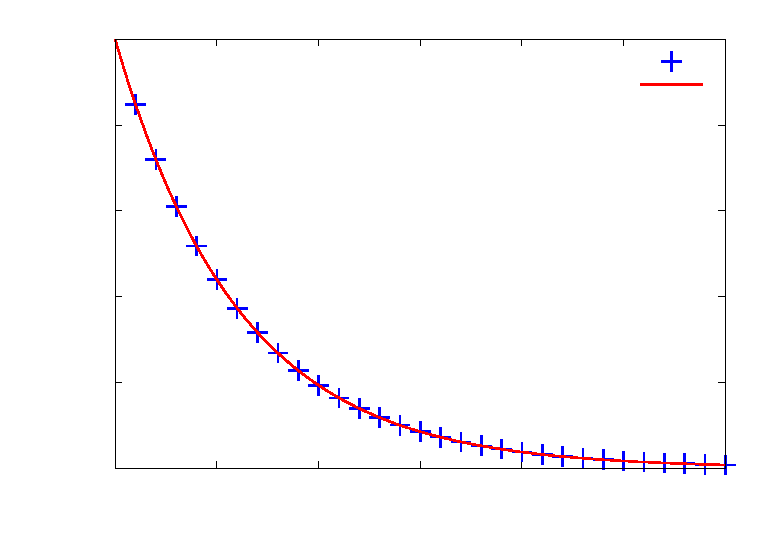
\includegraphics{plots/T2Kupfer250}}%
    \gplfronttext
  \end{picture}%
\endgroup

%     \caption{T2 Messung Kupfer $Cu^{2+} \SI{250}{\micro\mole}$}
% \end{figure}
% \begin{figure}[H]
%     \centering
%     % GNUPLOT: LaTeX picture with Postscript
\begingroup
  % Encoding inside the plot.  In the header of your document, this encoding
  % should to defined, e.g., by using
  % \usepackage[cp1252,<other encodings>]{inputenc}
  \inputencoding{cp1252}%
  \makeatletter
  \providecommand\color[2][]{%
    \GenericError{(gnuplot) \space\space\space\@spaces}{%
      Package color not loaded in conjunction with
      terminal option `colourtext'%
    }{See the gnuplot documentation for explanation.%
    }{Either use 'blacktext' in gnuplot or load the package
      color.sty in LaTeX.}%
    \renewcommand\color[2][]{}%
  }%
  \providecommand\includegraphics[2][]{%
    \GenericError{(gnuplot) \space\space\space\@spaces}{%
      Package graphicx or graphics not loaded%
    }{See the gnuplot documentation for explanation.%
    }{The gnuplot epslatex terminal needs graphicx.sty or graphics.sty.}%
    \renewcommand\includegraphics[2][]{}%
  }%
  \providecommand\rotatebox[2]{#2}%
  \@ifundefined{ifGPcolor}{%
    \newif\ifGPcolor
    \GPcolorfalse
  }{}%
  \@ifundefined{ifGPblacktext}{%
    \newif\ifGPblacktext
    \GPblacktexttrue
  }{}%
  % define a \g@addto@macro without @ in the name:
  \let\gplgaddtomacro\g@addto@macro
  % define empty templates for all commands taking text:
  \gdef\gplbacktext{}%
  \gdef\gplfronttext{}%
  \makeatother
  \ifGPblacktext
    % no textcolor at all
    \def\colorrgb#1{}%
    \def\colorgray#1{}%
  \else
    % gray or color?
    \ifGPcolor
      \def\colorrgb#1{\color[rgb]{#1}}%
      \def\colorgray#1{\color[gray]{#1}}%
      \expandafter\def\csname LTw\endcsname{\color{white}}%
      \expandafter\def\csname LTb\endcsname{\color{black}}%
      \expandafter\def\csname LTa\endcsname{\color{black}}%
      \expandafter\def\csname LT0\endcsname{\color[rgb]{1,0,0}}%
      \expandafter\def\csname LT1\endcsname{\color[rgb]{0,1,0}}%
      \expandafter\def\csname LT2\endcsname{\color[rgb]{0,0,1}}%
      \expandafter\def\csname LT3\endcsname{\color[rgb]{1,0,1}}%
      \expandafter\def\csname LT4\endcsname{\color[rgb]{0,1,1}}%
      \expandafter\def\csname LT5\endcsname{\color[rgb]{1,1,0}}%
      \expandafter\def\csname LT6\endcsname{\color[rgb]{0,0,0}}%
      \expandafter\def\csname LT7\endcsname{\color[rgb]{1,0.3,0}}%
      \expandafter\def\csname LT8\endcsname{\color[rgb]{0.5,0.5,0.5}}%
    \else
      % gray
      \def\colorrgb#1{\color{black}}%
      \def\colorgray#1{\color[gray]{#1}}%
      \expandafter\def\csname LTw\endcsname{\color{white}}%
      \expandafter\def\csname LTb\endcsname{\color{black}}%
      \expandafter\def\csname LTa\endcsname{\color{black}}%
      \expandafter\def\csname LT0\endcsname{\color{black}}%
      \expandafter\def\csname LT1\endcsname{\color{black}}%
      \expandafter\def\csname LT2\endcsname{\color{black}}%
      \expandafter\def\csname LT3\endcsname{\color{black}}%
      \expandafter\def\csname LT4\endcsname{\color{black}}%
      \expandafter\def\csname LT5\endcsname{\color{black}}%
      \expandafter\def\csname LT6\endcsname{\color{black}}%
      \expandafter\def\csname LT7\endcsname{\color{black}}%
      \expandafter\def\csname LT8\endcsname{\color{black}}%
    \fi
  \fi
    \setlength{\unitlength}{0.0500bp}%
    \ifx\gptboxheight\undefined%
      \newlength{\gptboxheight}%
      \newlength{\gptboxwidth}%
      \newsavebox{\gptboxtext}%
    \fi%
    \setlength{\fboxrule}{0.5pt}%
    \setlength{\fboxsep}{1pt}%
\begin{picture}(7200.00,5040.00)%
    \gplgaddtomacro\gplbacktext{%
      \csname LTb\endcsname%%
      \put(814,704){\makebox(0,0)[r]{\strut{}$0$}}%
      \put(814,1527){\makebox(0,0)[r]{\strut{}$0.2$}}%
      \put(814,2350){\makebox(0,0)[r]{\strut{}$0.4$}}%
      \put(814,3173){\makebox(0,0)[r]{\strut{}$0.6$}}%
      \put(814,3996){\makebox(0,0)[r]{\strut{}$0.8$}}%
      \put(814,4819){\makebox(0,0)[r]{\strut{}$1$}}%
      \put(946,484){\makebox(0,0){\strut{}$0$}}%
      \put(1563,484){\makebox(0,0){\strut{}$500$}}%
      \put(2179,484){\makebox(0,0){\strut{}$1000$}}%
      \put(2796,484){\makebox(0,0){\strut{}$1500$}}%
      \put(3412,484){\makebox(0,0){\strut{}$2000$}}%
      \put(4029,484){\makebox(0,0){\strut{}$2500$}}%
      \put(4645,484){\makebox(0,0){\strut{}$3000$}}%
      \put(5262,484){\makebox(0,0){\strut{}$3500$}}%
      \put(5878,484){\makebox(0,0){\strut{}$4000$}}%
      \put(6495,484){\makebox(0,0){\strut{}$4500$}}%
    }%
    \gplgaddtomacro\gplfronttext{%
      \csname LTb\endcsname%%
      \put(308,2761){\rotatebox{-270}{\makebox(0,0){\strut{}D\"ampfung $\frac{\text{E}}{\text{E}_0}$}}}%
      \put(3874,154){\makebox(0,0){\strut{}Zeit zwischen den Pulsen $t$ in $\si{\milli \second}$}}%
      \csname LTb\endcsname%%
      \put(5860,4606){\makebox(0,0)[r]{\strut{}gemessene Datenpunkte f\"ur $Cu^{2+} \SI{250}{\micro\mole}$}}%
      \csname LTb\endcsname%%
      \put(5860,4386){\makebox(0,0)[r]{\strut{}exponentieller Fit}}%
    }%
    \gplbacktext
    \put(0,0){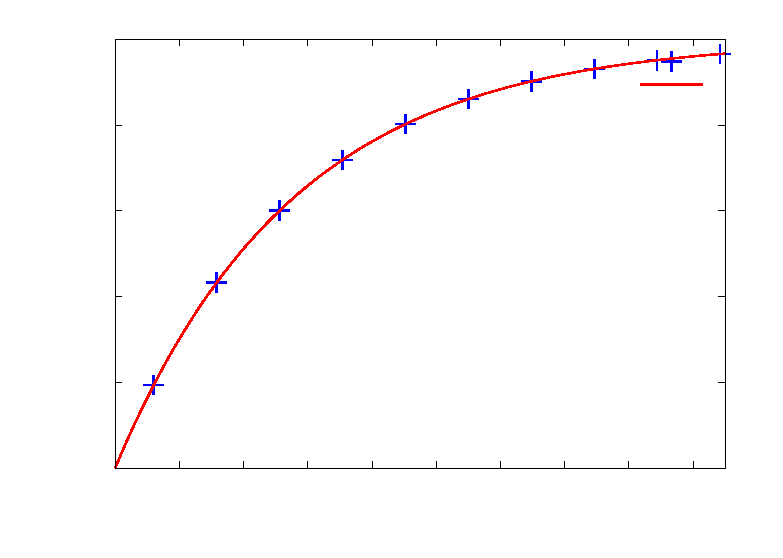
\includegraphics{plots/T1Kupfer250}}%
    \gplfronttext
  \end{picture}%
\endgroup

%     \caption{T1 Messung Kupfer $Cu^{2+} \SI{500}{\micro\mole}$}
% \end{figure}

% \begin{figure}[H]
%     \centering
%     % GNUPLOT: LaTeX picture with Postscript
\begingroup
  % Encoding inside the plot.  In the header of your document, this encoding
  % should to defined, e.g., by using
  % \usepackage[cp1252,<other encodings>]{inputenc}
  \inputencoding{cp1252}%
  \makeatletter
  \providecommand\color[2][]{%
    \GenericError{(gnuplot) \space\space\space\@spaces}{%
      Package color not loaded in conjunction with
      terminal option `colourtext'%
    }{See the gnuplot documentation for explanation.%
    }{Either use 'blacktext' in gnuplot or load the package
      color.sty in LaTeX.}%
    \renewcommand\color[2][]{}%
  }%
  \providecommand\includegraphics[2][]{%
    \GenericError{(gnuplot) \space\space\space\@spaces}{%
      Package graphicx or graphics not loaded%
    }{See the gnuplot documentation for explanation.%
    }{The gnuplot epslatex terminal needs graphicx.sty or graphics.sty.}%
    \renewcommand\includegraphics[2][]{}%
  }%
  \providecommand\rotatebox[2]{#2}%
  \@ifundefined{ifGPcolor}{%
    \newif\ifGPcolor
    \GPcolorfalse
  }{}%
  \@ifundefined{ifGPblacktext}{%
    \newif\ifGPblacktext
    \GPblacktexttrue
  }{}%
  % define a \g@addto@macro without @ in the name:
  \let\gplgaddtomacro\g@addto@macro
  % define empty templates for all commands taking text:
  \gdef\gplbacktext{}%
  \gdef\gplfronttext{}%
  \makeatother
  \ifGPblacktext
    % no textcolor at all
    \def\colorrgb#1{}%
    \def\colorgray#1{}%
  \else
    % gray or color?
    \ifGPcolor
      \def\colorrgb#1{\color[rgb]{#1}}%
      \def\colorgray#1{\color[gray]{#1}}%
      \expandafter\def\csname LTw\endcsname{\color{white}}%
      \expandafter\def\csname LTb\endcsname{\color{black}}%
      \expandafter\def\csname LTa\endcsname{\color{black}}%
      \expandafter\def\csname LT0\endcsname{\color[rgb]{1,0,0}}%
      \expandafter\def\csname LT1\endcsname{\color[rgb]{0,1,0}}%
      \expandafter\def\csname LT2\endcsname{\color[rgb]{0,0,1}}%
      \expandafter\def\csname LT3\endcsname{\color[rgb]{1,0,1}}%
      \expandafter\def\csname LT4\endcsname{\color[rgb]{0,1,1}}%
      \expandafter\def\csname LT5\endcsname{\color[rgb]{1,1,0}}%
      \expandafter\def\csname LT6\endcsname{\color[rgb]{0,0,0}}%
      \expandafter\def\csname LT7\endcsname{\color[rgb]{1,0.3,0}}%
      \expandafter\def\csname LT8\endcsname{\color[rgb]{0.5,0.5,0.5}}%
    \else
      % gray
      \def\colorrgb#1{\color{black}}%
      \def\colorgray#1{\color[gray]{#1}}%
      \expandafter\def\csname LTw\endcsname{\color{white}}%
      \expandafter\def\csname LTb\endcsname{\color{black}}%
      \expandafter\def\csname LTa\endcsname{\color{black}}%
      \expandafter\def\csname LT0\endcsname{\color{black}}%
      \expandafter\def\csname LT1\endcsname{\color{black}}%
      \expandafter\def\csname LT2\endcsname{\color{black}}%
      \expandafter\def\csname LT3\endcsname{\color{black}}%
      \expandafter\def\csname LT4\endcsname{\color{black}}%
      \expandafter\def\csname LT5\endcsname{\color{black}}%
      \expandafter\def\csname LT6\endcsname{\color{black}}%
      \expandafter\def\csname LT7\endcsname{\color{black}}%
      \expandafter\def\csname LT8\endcsname{\color{black}}%
    \fi
  \fi
    \setlength{\unitlength}{0.0500bp}%
    \ifx\gptboxheight\undefined%
      \newlength{\gptboxheight}%
      \newlength{\gptboxwidth}%
      \newsavebox{\gptboxtext}%
    \fi%
    \setlength{\fboxrule}{0.5pt}%
    \setlength{\fboxsep}{1pt}%
\begin{picture}(7200.00,5040.00)%
    \gplgaddtomacro\gplbacktext{%
      \csname LTb\endcsname%%
      \put(814,704){\makebox(0,0)[r]{\strut{}$0$}}%
      \put(814,1527){\makebox(0,0)[r]{\strut{}$0.2$}}%
      \put(814,2350){\makebox(0,0)[r]{\strut{}$0.4$}}%
      \put(814,3173){\makebox(0,0)[r]{\strut{}$0.6$}}%
      \put(814,3996){\makebox(0,0)[r]{\strut{}$0.8$}}%
      \put(814,4819){\makebox(0,0)[r]{\strut{}$1$}}%
      \put(946,484){\makebox(0,0){\strut{}$0$}}%
      \put(1922,484){\makebox(0,0){\strut{}$1000$}}%
      \put(2898,484){\makebox(0,0){\strut{}$2000$}}%
      \put(3875,484){\makebox(0,0){\strut{}$3000$}}%
      \put(4851,484){\makebox(0,0){\strut{}$4000$}}%
      \put(5827,484){\makebox(0,0){\strut{}$5000$}}%
      \put(6803,484){\makebox(0,0){\strut{}$6000$}}%
    }%
    \gplgaddtomacro\gplfronttext{%
      \csname LTb\endcsname%%
      \put(308,2761){\rotatebox{-270}{\makebox(0,0){\strut{}Dämpfung $\frac{\text{E}}{\text{E}_0}$}}}%
      \put(3874,154){\makebox(0,0){\strut{}Zeit in $\si{\milli \second}$}}%
      \csname LTb\endcsname%%
      \put(5816,4646){\makebox(0,0)[r]{\strut{}gemessene Datenpunkte für $Cu^{2+} \SI{250}{\micro\mole}$}}%
      \csname LTb\endcsname%%
      \put(5816,4426){\makebox(0,0)[r]{\strut{}Dämpfungsfit Fit}}%
    }%
    \gplbacktext
    \put(0,0){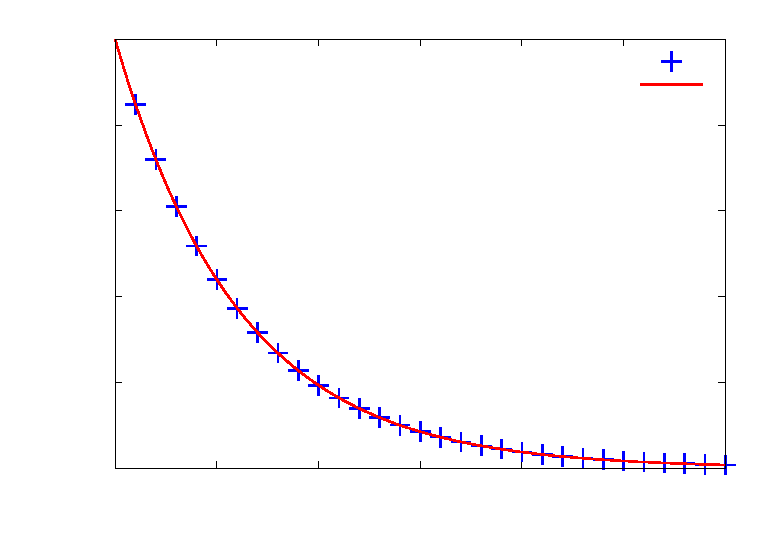
\includegraphics{plots/T2Kupfer250}}%
    \gplfronttext
  \end{picture}%
\endgroup

%     \caption{T2 Messung Kupfer $Cu^{2+} \SI{500}{\micro\mole}$}
% \end{figure}
% \begin{figure}[H]
%     \centering
%     % GNUPLOT: LaTeX picture with Postscript
\begingroup
  % Encoding inside the plot.  In the header of your document, this encoding
  % should to defined, e.g., by using
  % \usepackage[cp1252,<other encodings>]{inputenc}
  \inputencoding{cp1252}%
  \makeatletter
  \providecommand\color[2][]{%
    \GenericError{(gnuplot) \space\space\space\@spaces}{%
      Package color not loaded in conjunction with
      terminal option `colourtext'%
    }{See the gnuplot documentation for explanation.%
    }{Either use 'blacktext' in gnuplot or load the package
      color.sty in LaTeX.}%
    \renewcommand\color[2][]{}%
  }%
  \providecommand\includegraphics[2][]{%
    \GenericError{(gnuplot) \space\space\space\@spaces}{%
      Package graphicx or graphics not loaded%
    }{See the gnuplot documentation for explanation.%
    }{The gnuplot epslatex terminal needs graphicx.sty or graphics.sty.}%
    \renewcommand\includegraphics[2][]{}%
  }%
  \providecommand\rotatebox[2]{#2}%
  \@ifundefined{ifGPcolor}{%
    \newif\ifGPcolor
    \GPcolorfalse
  }{}%
  \@ifundefined{ifGPblacktext}{%
    \newif\ifGPblacktext
    \GPblacktexttrue
  }{}%
  % define a \g@addto@macro without @ in the name:
  \let\gplgaddtomacro\g@addto@macro
  % define empty templates for all commands taking text:
  \gdef\gplbacktext{}%
  \gdef\gplfronttext{}%
  \makeatother
  \ifGPblacktext
    % no textcolor at all
    \def\colorrgb#1{}%
    \def\colorgray#1{}%
  \else
    % gray or color?
    \ifGPcolor
      \def\colorrgb#1{\color[rgb]{#1}}%
      \def\colorgray#1{\color[gray]{#1}}%
      \expandafter\def\csname LTw\endcsname{\color{white}}%
      \expandafter\def\csname LTb\endcsname{\color{black}}%
      \expandafter\def\csname LTa\endcsname{\color{black}}%
      \expandafter\def\csname LT0\endcsname{\color[rgb]{1,0,0}}%
      \expandafter\def\csname LT1\endcsname{\color[rgb]{0,1,0}}%
      \expandafter\def\csname LT2\endcsname{\color[rgb]{0,0,1}}%
      \expandafter\def\csname LT3\endcsname{\color[rgb]{1,0,1}}%
      \expandafter\def\csname LT4\endcsname{\color[rgb]{0,1,1}}%
      \expandafter\def\csname LT5\endcsname{\color[rgb]{1,1,0}}%
      \expandafter\def\csname LT6\endcsname{\color[rgb]{0,0,0}}%
      \expandafter\def\csname LT7\endcsname{\color[rgb]{1,0.3,0}}%
      \expandafter\def\csname LT8\endcsname{\color[rgb]{0.5,0.5,0.5}}%
    \else
      % gray
      \def\colorrgb#1{\color{black}}%
      \def\colorgray#1{\color[gray]{#1}}%
      \expandafter\def\csname LTw\endcsname{\color{white}}%
      \expandafter\def\csname LTb\endcsname{\color{black}}%
      \expandafter\def\csname LTa\endcsname{\color{black}}%
      \expandafter\def\csname LT0\endcsname{\color{black}}%
      \expandafter\def\csname LT1\endcsname{\color{black}}%
      \expandafter\def\csname LT2\endcsname{\color{black}}%
      \expandafter\def\csname LT3\endcsname{\color{black}}%
      \expandafter\def\csname LT4\endcsname{\color{black}}%
      \expandafter\def\csname LT5\endcsname{\color{black}}%
      \expandafter\def\csname LT6\endcsname{\color{black}}%
      \expandafter\def\csname LT7\endcsname{\color{black}}%
      \expandafter\def\csname LT8\endcsname{\color{black}}%
    \fi
  \fi
    \setlength{\unitlength}{0.0500bp}%
    \ifx\gptboxheight\undefined%
      \newlength{\gptboxheight}%
      \newlength{\gptboxwidth}%
      \newsavebox{\gptboxtext}%
    \fi%
    \setlength{\fboxrule}{0.5pt}%
    \setlength{\fboxsep}{1pt}%
\begin{picture}(7200.00,5040.00)%
    \gplgaddtomacro\gplbacktext{%
      \csname LTb\endcsname%%
      \put(814,704){\makebox(0,0)[r]{\strut{}$0$}}%
      \put(814,1527){\makebox(0,0)[r]{\strut{}$0.2$}}%
      \put(814,2350){\makebox(0,0)[r]{\strut{}$0.4$}}%
      \put(814,3173){\makebox(0,0)[r]{\strut{}$0.6$}}%
      \put(814,3996){\makebox(0,0)[r]{\strut{}$0.8$}}%
      \put(814,4819){\makebox(0,0)[r]{\strut{}$1$}}%
      \put(946,484){\makebox(0,0){\strut{}$0$}}%
      \put(1563,484){\makebox(0,0){\strut{}$500$}}%
      \put(2179,484){\makebox(0,0){\strut{}$1000$}}%
      \put(2796,484){\makebox(0,0){\strut{}$1500$}}%
      \put(3412,484){\makebox(0,0){\strut{}$2000$}}%
      \put(4029,484){\makebox(0,0){\strut{}$2500$}}%
      \put(4645,484){\makebox(0,0){\strut{}$3000$}}%
      \put(5262,484){\makebox(0,0){\strut{}$3500$}}%
      \put(5878,484){\makebox(0,0){\strut{}$4000$}}%
      \put(6495,484){\makebox(0,0){\strut{}$4500$}}%
    }%
    \gplgaddtomacro\gplfronttext{%
      \csname LTb\endcsname%%
      \put(308,2761){\rotatebox{-270}{\makebox(0,0){\strut{}D\"ampfung $\frac{\text{E}}{\text{E}_0}$}}}%
      \put(3874,154){\makebox(0,0){\strut{}Zeit zwischen den Pulsen $t$ in $\si{\milli \second}$}}%
      \csname LTb\endcsname%%
      \put(5860,4606){\makebox(0,0)[r]{\strut{}gemessene Datenpunkte f\"ur $Cu^{2+} \SI{250}{\micro\mole}$}}%
      \csname LTb\endcsname%%
      \put(5860,4386){\makebox(0,0)[r]{\strut{}exponentieller Fit}}%
    }%
    \gplbacktext
    \put(0,0){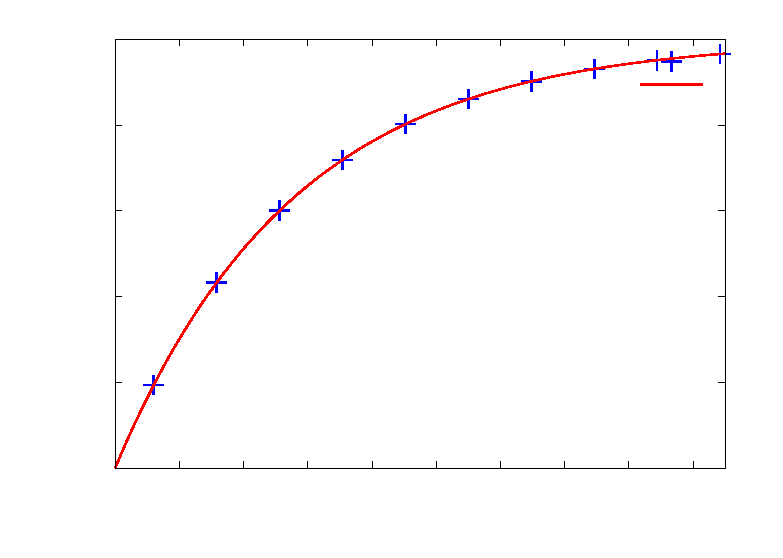
\includegraphics{plots/T1Kupfer250}}%
    \gplfronttext
  \end{picture}%
\endgroup

%     \caption{T1 Messung Kupfer $Cu^{2+} \SI{1000}{\micro\mole}$}
% \end{figure}

% \begin{figure}[H]
%     \centering
%     % GNUPLOT: LaTeX picture with Postscript
\begingroup
  % Encoding inside the plot.  In the header of your document, this encoding
  % should to defined, e.g., by using
  % \usepackage[cp1252,<other encodings>]{inputenc}
  \inputencoding{cp1252}%
  \makeatletter
  \providecommand\color[2][]{%
    \GenericError{(gnuplot) \space\space\space\@spaces}{%
      Package color not loaded in conjunction with
      terminal option `colourtext'%
    }{See the gnuplot documentation for explanation.%
    }{Either use 'blacktext' in gnuplot or load the package
      color.sty in LaTeX.}%
    \renewcommand\color[2][]{}%
  }%
  \providecommand\includegraphics[2][]{%
    \GenericError{(gnuplot) \space\space\space\@spaces}{%
      Package graphicx or graphics not loaded%
    }{See the gnuplot documentation for explanation.%
    }{The gnuplot epslatex terminal needs graphicx.sty or graphics.sty.}%
    \renewcommand\includegraphics[2][]{}%
  }%
  \providecommand\rotatebox[2]{#2}%
  \@ifundefined{ifGPcolor}{%
    \newif\ifGPcolor
    \GPcolorfalse
  }{}%
  \@ifundefined{ifGPblacktext}{%
    \newif\ifGPblacktext
    \GPblacktexttrue
  }{}%
  % define a \g@addto@macro without @ in the name:
  \let\gplgaddtomacro\g@addto@macro
  % define empty templates for all commands taking text:
  \gdef\gplbacktext{}%
  \gdef\gplfronttext{}%
  \makeatother
  \ifGPblacktext
    % no textcolor at all
    \def\colorrgb#1{}%
    \def\colorgray#1{}%
  \else
    % gray or color?
    \ifGPcolor
      \def\colorrgb#1{\color[rgb]{#1}}%
      \def\colorgray#1{\color[gray]{#1}}%
      \expandafter\def\csname LTw\endcsname{\color{white}}%
      \expandafter\def\csname LTb\endcsname{\color{black}}%
      \expandafter\def\csname LTa\endcsname{\color{black}}%
      \expandafter\def\csname LT0\endcsname{\color[rgb]{1,0,0}}%
      \expandafter\def\csname LT1\endcsname{\color[rgb]{0,1,0}}%
      \expandafter\def\csname LT2\endcsname{\color[rgb]{0,0,1}}%
      \expandafter\def\csname LT3\endcsname{\color[rgb]{1,0,1}}%
      \expandafter\def\csname LT4\endcsname{\color[rgb]{0,1,1}}%
      \expandafter\def\csname LT5\endcsname{\color[rgb]{1,1,0}}%
      \expandafter\def\csname LT6\endcsname{\color[rgb]{0,0,0}}%
      \expandafter\def\csname LT7\endcsname{\color[rgb]{1,0.3,0}}%
      \expandafter\def\csname LT8\endcsname{\color[rgb]{0.5,0.5,0.5}}%
    \else
      % gray
      \def\colorrgb#1{\color{black}}%
      \def\colorgray#1{\color[gray]{#1}}%
      \expandafter\def\csname LTw\endcsname{\color{white}}%
      \expandafter\def\csname LTb\endcsname{\color{black}}%
      \expandafter\def\csname LTa\endcsname{\color{black}}%
      \expandafter\def\csname LT0\endcsname{\color{black}}%
      \expandafter\def\csname LT1\endcsname{\color{black}}%
      \expandafter\def\csname LT2\endcsname{\color{black}}%
      \expandafter\def\csname LT3\endcsname{\color{black}}%
      \expandafter\def\csname LT4\endcsname{\color{black}}%
      \expandafter\def\csname LT5\endcsname{\color{black}}%
      \expandafter\def\csname LT6\endcsname{\color{black}}%
      \expandafter\def\csname LT7\endcsname{\color{black}}%
      \expandafter\def\csname LT8\endcsname{\color{black}}%
    \fi
  \fi
    \setlength{\unitlength}{0.0500bp}%
    \ifx\gptboxheight\undefined%
      \newlength{\gptboxheight}%
      \newlength{\gptboxwidth}%
      \newsavebox{\gptboxtext}%
    \fi%
    \setlength{\fboxrule}{0.5pt}%
    \setlength{\fboxsep}{1pt}%
\begin{picture}(7200.00,5040.00)%
    \gplgaddtomacro\gplbacktext{%
      \csname LTb\endcsname%%
      \put(814,704){\makebox(0,0)[r]{\strut{}$0$}}%
      \put(814,1527){\makebox(0,0)[r]{\strut{}$0.2$}}%
      \put(814,2350){\makebox(0,0)[r]{\strut{}$0.4$}}%
      \put(814,3173){\makebox(0,0)[r]{\strut{}$0.6$}}%
      \put(814,3996){\makebox(0,0)[r]{\strut{}$0.8$}}%
      \put(814,4819){\makebox(0,0)[r]{\strut{}$1$}}%
      \put(946,484){\makebox(0,0){\strut{}$0$}}%
      \put(1922,484){\makebox(0,0){\strut{}$1000$}}%
      \put(2898,484){\makebox(0,0){\strut{}$2000$}}%
      \put(3875,484){\makebox(0,0){\strut{}$3000$}}%
      \put(4851,484){\makebox(0,0){\strut{}$4000$}}%
      \put(5827,484){\makebox(0,0){\strut{}$5000$}}%
      \put(6803,484){\makebox(0,0){\strut{}$6000$}}%
    }%
    \gplgaddtomacro\gplfronttext{%
      \csname LTb\endcsname%%
      \put(308,2761){\rotatebox{-270}{\makebox(0,0){\strut{}Dämpfung $\frac{\text{E}}{\text{E}_0}$}}}%
      \put(3874,154){\makebox(0,0){\strut{}Zeit in $\si{\milli \second}$}}%
      \csname LTb\endcsname%%
      \put(5816,4646){\makebox(0,0)[r]{\strut{}gemessene Datenpunkte für $Cu^{2+} \SI{250}{\micro\mole}$}}%
      \csname LTb\endcsname%%
      \put(5816,4426){\makebox(0,0)[r]{\strut{}Dämpfungsfit Fit}}%
    }%
    \gplbacktext
    \put(0,0){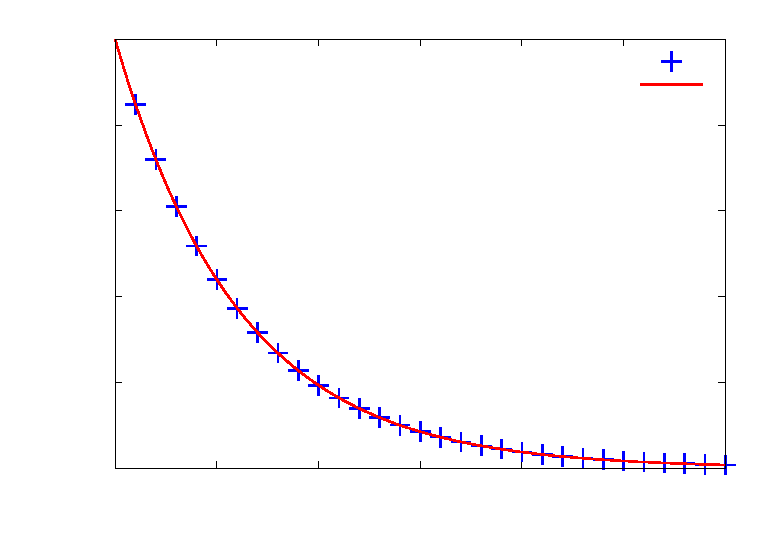
\includegraphics{plots/T2Kupfer250}}%
    \gplfronttext
  \end{picture}%
\endgroup

%     \caption{T2 Messung Kupfer $Cu^{2+} \SI{1000}{\micro\mole}$}
% \end{figure}

\begin{figure}[H]
    \centering
    % GNUPLOT: LaTeX picture with Postscript
\begingroup
  % Encoding inside the plot.  In the header of your document, this encoding
  % should to defined, e.g., by using
  % \usepackage[cp1252,<other encodings>]{inputenc}
  \inputencoding{cp1252}%
  \makeatletter
  \providecommand\color[2][]{%
    \GenericError{(gnuplot) \space\space\space\@spaces}{%
      Package color not loaded in conjunction with
      terminal option `colourtext'%
    }{See the gnuplot documentation for explanation.%
    }{Either use 'blacktext' in gnuplot or load the package
      color.sty in LaTeX.}%
    \renewcommand\color[2][]{}%
  }%
  \providecommand\includegraphics[2][]{%
    \GenericError{(gnuplot) \space\space\space\@spaces}{%
      Package graphicx or graphics not loaded%
    }{See the gnuplot documentation for explanation.%
    }{The gnuplot epslatex terminal needs graphicx.sty or graphics.sty.}%
    \renewcommand\includegraphics[2][]{}%
  }%
  \providecommand\rotatebox[2]{#2}%
  \@ifundefined{ifGPcolor}{%
    \newif\ifGPcolor
    \GPcolorfalse
  }{}%
  \@ifundefined{ifGPblacktext}{%
    \newif\ifGPblacktext
    \GPblacktexttrue
  }{}%
  % define a \g@addto@macro without @ in the name:
  \let\gplgaddtomacro\g@addto@macro
  % define empty templates for all commands taking text:
  \gdef\gplbacktext{}%
  \gdef\gplfronttext{}%
  \makeatother
  \ifGPblacktext
    % no textcolor at all
    \def\colorrgb#1{}%
    \def\colorgray#1{}%
  \else
    % gray or color?
    \ifGPcolor
      \def\colorrgb#1{\color[rgb]{#1}}%
      \def\colorgray#1{\color[gray]{#1}}%
      \expandafter\def\csname LTw\endcsname{\color{white}}%
      \expandafter\def\csname LTb\endcsname{\color{black}}%
      \expandafter\def\csname LTa\endcsname{\color{black}}%
      \expandafter\def\csname LT0\endcsname{\color[rgb]{1,0,0}}%
      \expandafter\def\csname LT1\endcsname{\color[rgb]{0,1,0}}%
      \expandafter\def\csname LT2\endcsname{\color[rgb]{0,0,1}}%
      \expandafter\def\csname LT3\endcsname{\color[rgb]{1,0,1}}%
      \expandafter\def\csname LT4\endcsname{\color[rgb]{0,1,1}}%
      \expandafter\def\csname LT5\endcsname{\color[rgb]{1,1,0}}%
      \expandafter\def\csname LT6\endcsname{\color[rgb]{0,0,0}}%
      \expandafter\def\csname LT7\endcsname{\color[rgb]{1,0.3,0}}%
      \expandafter\def\csname LT8\endcsname{\color[rgb]{0.5,0.5,0.5}}%
    \else
      % gray
      \def\colorrgb#1{\color{black}}%
      \def\colorgray#1{\color[gray]{#1}}%
      \expandafter\def\csname LTw\endcsname{\color{white}}%
      \expandafter\def\csname LTb\endcsname{\color{black}}%
      \expandafter\def\csname LTa\endcsname{\color{black}}%
      \expandafter\def\csname LT0\endcsname{\color{black}}%
      \expandafter\def\csname LT1\endcsname{\color{black}}%
      \expandafter\def\csname LT2\endcsname{\color{black}}%
      \expandafter\def\csname LT3\endcsname{\color{black}}%
      \expandafter\def\csname LT4\endcsname{\color{black}}%
      \expandafter\def\csname LT5\endcsname{\color{black}}%
      \expandafter\def\csname LT6\endcsname{\color{black}}%
      \expandafter\def\csname LT7\endcsname{\color{black}}%
      \expandafter\def\csname LT8\endcsname{\color{black}}%
    \fi
  \fi
    \setlength{\unitlength}{0.0500bp}%
    \ifx\gptboxheight\undefined%
      \newlength{\gptboxheight}%
      \newlength{\gptboxwidth}%
      \newsavebox{\gptboxtext}%
    \fi%
    \setlength{\fboxrule}{0.5pt}%
    \setlength{\fboxsep}{1pt}%
\begin{picture}(7200.00,5040.00)%
    \gplgaddtomacro\gplbacktext{%
      \csname LTb\endcsname%%
      \put(814,704){\makebox(0,0)[r]{\strut{}$0$}}%
      \put(814,1527){\makebox(0,0)[r]{\strut{}$0.2$}}%
      \put(814,2350){\makebox(0,0)[r]{\strut{}$0.4$}}%
      \put(814,3173){\makebox(0,0)[r]{\strut{}$0.6$}}%
      \put(814,3996){\makebox(0,0)[r]{\strut{}$0.8$}}%
      \put(814,4819){\makebox(0,0)[r]{\strut{}$1$}}%
      \put(946,484){\makebox(0,0){\strut{}$0$}}%
      \put(1922,484){\makebox(0,0){\strut{}$1000$}}%
      \put(2898,484){\makebox(0,0){\strut{}$2000$}}%
      \put(3875,484){\makebox(0,0){\strut{}$3000$}}%
      \put(4851,484){\makebox(0,0){\strut{}$4000$}}%
      \put(5827,484){\makebox(0,0){\strut{}$5000$}}%
      \put(6803,484){\makebox(0,0){\strut{}$6000$}}%
    }%
    \gplgaddtomacro\gplfronttext{%
      \csname LTb\endcsname%%
      \put(308,2761){\rotatebox{-270}{\makebox(0,0){\strut{}Dämpfung $\frac{\text{E}}{\text{E}_0}$}}}%
      \put(3874,154){\makebox(0,0){\strut{}Zeit in $\si{\milli \second}$}}%
      \csname LTb\endcsname%%
      \put(5889,3886){\makebox(0,0)[r]{\strut{}$Cu^{2+} \SI{250}{\micro\mole}$}}%
      \csname LTb\endcsname%%
      \put(5889,3666){\makebox(0,0)[r]{\strut{}$Cu^{2+} \SI{500}{\micro\mole}$}}%
      \csname LTb\endcsname%%
      \put(5889,3446){\makebox(0,0)[r]{\strut{}$Cu^{2+} \SI{1000}{\micro\mole}$}}%
      \csname LTb\endcsname%%
      \put(5889,3226){\makebox(0,0)[r]{\strut{}$Cu^{2+} \SI{2000}{\micro\mole}$}}%
      \csname LTb\endcsname%%
      \put(5889,3006){\makebox(0,0)[r]{\strut{}Wasser}}%
    }%
    \gplbacktext
    \put(0,0){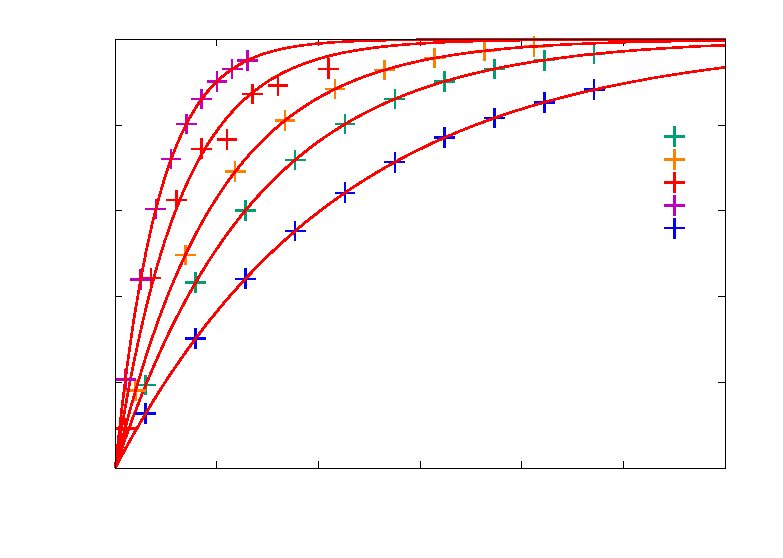
\includegraphics{plots/KupferalleT1}}%
    \gplfronttext
  \end{picture}%
\endgroup

    \caption{Alle Messungen T1 Cu2+}
\end{figure}
\begin{figure}[H]
    \centering
    % GNUPLOT: LaTeX picture with Postscript
\begingroup
  % Encoding inside the plot.  In the header of your document, this encoding
  % should to defined, e.g., by using
  % \usepackage[cp1252,<other encodings>]{inputenc}
  \inputencoding{cp1252}%
  \makeatletter
  \providecommand\color[2][]{%
    \GenericError{(gnuplot) \space\space\space\@spaces}{%
      Package color not loaded in conjunction with
      terminal option `colourtext'%
    }{See the gnuplot documentation for explanation.%
    }{Either use 'blacktext' in gnuplot or load the package
      color.sty in LaTeX.}%
    \renewcommand\color[2][]{}%
  }%
  \providecommand\includegraphics[2][]{%
    \GenericError{(gnuplot) \space\space\space\@spaces}{%
      Package graphicx or graphics not loaded%
    }{See the gnuplot documentation for explanation.%
    }{The gnuplot epslatex terminal needs graphicx.sty or graphics.sty.}%
    \renewcommand\includegraphics[2][]{}%
  }%
  \providecommand\rotatebox[2]{#2}%
  \@ifundefined{ifGPcolor}{%
    \newif\ifGPcolor
    \GPcolorfalse
  }{}%
  \@ifundefined{ifGPblacktext}{%
    \newif\ifGPblacktext
    \GPblacktexttrue
  }{}%
  % define a \g@addto@macro without @ in the name:
  \let\gplgaddtomacro\g@addto@macro
  % define empty templates for all commands taking text:
  \gdef\gplbacktext{}%
  \gdef\gplfronttext{}%
  \makeatother
  \ifGPblacktext
    % no textcolor at all
    \def\colorrgb#1{}%
    \def\colorgray#1{}%
  \else
    % gray or color?
    \ifGPcolor
      \def\colorrgb#1{\color[rgb]{#1}}%
      \def\colorgray#1{\color[gray]{#1}}%
      \expandafter\def\csname LTw\endcsname{\color{white}}%
      \expandafter\def\csname LTb\endcsname{\color{black}}%
      \expandafter\def\csname LTa\endcsname{\color{black}}%
      \expandafter\def\csname LT0\endcsname{\color[rgb]{1,0,0}}%
      \expandafter\def\csname LT1\endcsname{\color[rgb]{0,1,0}}%
      \expandafter\def\csname LT2\endcsname{\color[rgb]{0,0,1}}%
      \expandafter\def\csname LT3\endcsname{\color[rgb]{1,0,1}}%
      \expandafter\def\csname LT4\endcsname{\color[rgb]{0,1,1}}%
      \expandafter\def\csname LT5\endcsname{\color[rgb]{1,1,0}}%
      \expandafter\def\csname LT6\endcsname{\color[rgb]{0,0,0}}%
      \expandafter\def\csname LT7\endcsname{\color[rgb]{1,0.3,0}}%
      \expandafter\def\csname LT8\endcsname{\color[rgb]{0.5,0.5,0.5}}%
    \else
      % gray
      \def\colorrgb#1{\color{black}}%
      \def\colorgray#1{\color[gray]{#1}}%
      \expandafter\def\csname LTw\endcsname{\color{white}}%
      \expandafter\def\csname LTb\endcsname{\color{black}}%
      \expandafter\def\csname LTa\endcsname{\color{black}}%
      \expandafter\def\csname LT0\endcsname{\color{black}}%
      \expandafter\def\csname LT1\endcsname{\color{black}}%
      \expandafter\def\csname LT2\endcsname{\color{black}}%
      \expandafter\def\csname LT3\endcsname{\color{black}}%
      \expandafter\def\csname LT4\endcsname{\color{black}}%
      \expandafter\def\csname LT5\endcsname{\color{black}}%
      \expandafter\def\csname LT6\endcsname{\color{black}}%
      \expandafter\def\csname LT7\endcsname{\color{black}}%
      \expandafter\def\csname LT8\endcsname{\color{black}}%
    \fi
  \fi
    \setlength{\unitlength}{0.0500bp}%
    \ifx\gptboxheight\undefined%
      \newlength{\gptboxheight}%
      \newlength{\gptboxwidth}%
      \newsavebox{\gptboxtext}%
    \fi%
    \setlength{\fboxrule}{0.5pt}%
    \setlength{\fboxsep}{1pt}%
\begin{picture}(7200.00,5040.00)%
    \gplgaddtomacro\gplbacktext{%
      \csname LTb\endcsname%%
      \put(814,704){\makebox(0,0)[r]{\strut{}$0$}}%
      \put(814,1527){\makebox(0,0)[r]{\strut{}$0.2$}}%
      \put(814,2350){\makebox(0,0)[r]{\strut{}$0.4$}}%
      \put(814,3173){\makebox(0,0)[r]{\strut{}$0.6$}}%
      \put(814,3996){\makebox(0,0)[r]{\strut{}$0.8$}}%
      \put(814,4819){\makebox(0,0)[r]{\strut{}$1$}}%
      \put(946,484){\makebox(0,0){\strut{}$0$}}%
      \put(1922,484){\makebox(0,0){\strut{}$1000$}}%
      \put(2898,484){\makebox(0,0){\strut{}$2000$}}%
      \put(3875,484){\makebox(0,0){\strut{}$3000$}}%
      \put(4851,484){\makebox(0,0){\strut{}$4000$}}%
      \put(5827,484){\makebox(0,0){\strut{}$5000$}}%
      \put(6803,484){\makebox(0,0){\strut{}$6000$}}%
    }%
    \gplgaddtomacro\gplfronttext{%
      \csname LTb\endcsname%%
      \put(308,2761){\rotatebox{-270}{\makebox(0,0){\strut{}D\"ampfung $\frac{\text{E}}{\text{E}_0}$}}}%
      \put(3874,154){\makebox(0,0){\strut{}Zeit in $\si{\milli \second}$}}%
      \csname LTb\endcsname%%
      \put(5860,4606){\makebox(0,0)[r]{\strut{}$Cu^{2+} \SI{250}{\micro\mole}$}}%
      \csname LTb\endcsname%%
      \put(5860,4386){\makebox(0,0)[r]{\strut{}$Cu^{2+} \SI{1000}{\micro\mole}$}}%
      \csname LTb\endcsname%%
      \put(5860,4166){\makebox(0,0)[r]{\strut{}$Cu^{2+} \SI{250}{\micro\mole}$}}%
      \csname LTb\endcsname%%
      \put(5860,3946){\makebox(0,0)[r]{\strut{}$Cu^{2+} \SI{2000}{\micro\mole}$}}%
      \csname LTb\endcsname%%
      \put(5860,3726){\makebox(0,0)[r]{\strut{}Wasser}}%
    }%
    \gplbacktext
    \put(0,0){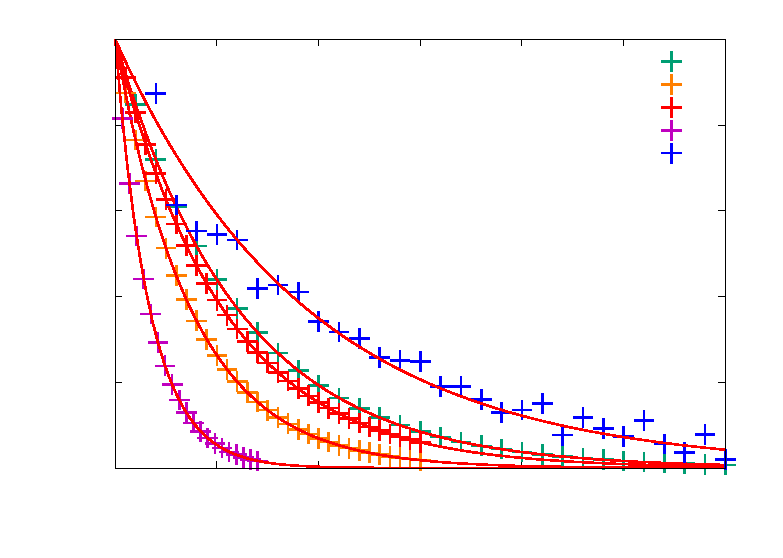
\includegraphics{plots/KupferalleT2}}%
    \gplfronttext
  \end{picture}%
\endgroup

    \caption{Alle Messungen T2Cu2+}
\end{figure}
\begin{figure}[H]
    \centering
    % GNUPLOT: LaTeX picture with Postscript
\begingroup
  % Encoding inside the plot.  In the header of your document, this encoding
  % should to defined, e.g., by using
  % \usepackage[cp1252,<other encodings>]{inputenc}
  \inputencoding{cp1252}%
  \makeatletter
  \providecommand\color[2][]{%
    \GenericError{(gnuplot) \space\space\space\@spaces}{%
      Package color not loaded in conjunction with
      terminal option `colourtext'%
    }{See the gnuplot documentation for explanation.%
    }{Either use 'blacktext' in gnuplot or load the package
      color.sty in LaTeX.}%
    \renewcommand\color[2][]{}%
  }%
  \providecommand\includegraphics[2][]{%
    \GenericError{(gnuplot) \space\space\space\@spaces}{%
      Package graphicx or graphics not loaded%
    }{See the gnuplot documentation for explanation.%
    }{The gnuplot epslatex terminal needs graphicx.sty or graphics.sty.}%
    \renewcommand\includegraphics[2][]{}%
  }%
  \providecommand\rotatebox[2]{#2}%
  \@ifundefined{ifGPcolor}{%
    \newif\ifGPcolor
    \GPcolorfalse
  }{}%
  \@ifundefined{ifGPblacktext}{%
    \newif\ifGPblacktext
    \GPblacktexttrue
  }{}%
  % define a \g@addto@macro without @ in the name:
  \let\gplgaddtomacro\g@addto@macro
  % define empty templates for all commands taking text:
  \gdef\gplbacktext{}%
  \gdef\gplfronttext{}%
  \makeatother
  \ifGPblacktext
    % no textcolor at all
    \def\colorrgb#1{}%
    \def\colorgray#1{}%
  \else
    % gray or color?
    \ifGPcolor
      \def\colorrgb#1{\color[rgb]{#1}}%
      \def\colorgray#1{\color[gray]{#1}}%
      \expandafter\def\csname LTw\endcsname{\color{white}}%
      \expandafter\def\csname LTb\endcsname{\color{black}}%
      \expandafter\def\csname LTa\endcsname{\color{black}}%
      \expandafter\def\csname LT0\endcsname{\color[rgb]{1,0,0}}%
      \expandafter\def\csname LT1\endcsname{\color[rgb]{0,1,0}}%
      \expandafter\def\csname LT2\endcsname{\color[rgb]{0,0,1}}%
      \expandafter\def\csname LT3\endcsname{\color[rgb]{1,0,1}}%
      \expandafter\def\csname LT4\endcsname{\color[rgb]{0,1,1}}%
      \expandafter\def\csname LT5\endcsname{\color[rgb]{1,1,0}}%
      \expandafter\def\csname LT6\endcsname{\color[rgb]{0,0,0}}%
      \expandafter\def\csname LT7\endcsname{\color[rgb]{1,0.3,0}}%
      \expandafter\def\csname LT8\endcsname{\color[rgb]{0.5,0.5,0.5}}%
    \else
      % gray
      \def\colorrgb#1{\color{black}}%
      \def\colorgray#1{\color[gray]{#1}}%
      \expandafter\def\csname LTw\endcsname{\color{white}}%
      \expandafter\def\csname LTb\endcsname{\color{black}}%
      \expandafter\def\csname LTa\endcsname{\color{black}}%
      \expandafter\def\csname LT0\endcsname{\color{black}}%
      \expandafter\def\csname LT1\endcsname{\color{black}}%
      \expandafter\def\csname LT2\endcsname{\color{black}}%
      \expandafter\def\csname LT3\endcsname{\color{black}}%
      \expandafter\def\csname LT4\endcsname{\color{black}}%
      \expandafter\def\csname LT5\endcsname{\color{black}}%
      \expandafter\def\csname LT6\endcsname{\color{black}}%
      \expandafter\def\csname LT7\endcsname{\color{black}}%
      \expandafter\def\csname LT8\endcsname{\color{black}}%
    \fi
  \fi
    \setlength{\unitlength}{0.0500bp}%
    \ifx\gptboxheight\undefined%
      \newlength{\gptboxheight}%
      \newlength{\gptboxwidth}%
      \newsavebox{\gptboxtext}%
    \fi%
    \setlength{\fboxrule}{0.5pt}%
    \setlength{\fboxsep}{1pt}%
\begin{picture}(7200.00,5040.00)%
    \gplgaddtomacro\gplbacktext{%
      \csname LTb\endcsname%%
      \put(814,704){\makebox(0,0)[r]{\strut{}$0$}}%
      \put(814,1527){\makebox(0,0)[r]{\strut{}$0.2$}}%
      \put(814,2350){\makebox(0,0)[r]{\strut{}$0.4$}}%
      \put(814,3173){\makebox(0,0)[r]{\strut{}$0.6$}}%
      \put(814,3996){\makebox(0,0)[r]{\strut{}$0.8$}}%
      \put(814,4819){\makebox(0,0)[r]{\strut{}$1$}}%
      \put(946,484){\makebox(0,0){\strut{}$0$}}%
      \put(1922,484){\makebox(0,0){\strut{}$1000$}}%
      \put(2898,484){\makebox(0,0){\strut{}$2000$}}%
      \put(3875,484){\makebox(0,0){\strut{}$3000$}}%
      \put(4851,484){\makebox(0,0){\strut{}$4000$}}%
      \put(5827,484){\makebox(0,0){\strut{}$5000$}}%
      \put(6803,484){\makebox(0,0){\strut{}$6000$}}%
    }%
    \gplgaddtomacro\gplfronttext{%
      \csname LTb\endcsname%%
      \put(198,2761){\rotatebox{-270}{\makebox(0,0){\strut{}D\"ampfung $\frac{\text{E}}{\text{E}_0}$}}}%
      \put(3874,154){\makebox(0,0){\strut{}Zeit in $\si{\milli \second}$}}%
      \csname LTb\endcsname%%
      \put(5860,3680){\makebox(0,0)[r]{\strut{}$Mn^{2+} \SI{25}{\micro\mole}$}}%
      \csname LTb\endcsname%%
      \put(5860,3460){\makebox(0,0)[r]{\strut{}$Mn^{2+} \SI{50}{\micro\mole}$}}%
      \csname LTb\endcsname%%
      \put(5860,3240){\makebox(0,0)[r]{\strut{}$Mn^{2+} \SI{100}{\micro\mole}$}}%
      \csname LTb\endcsname%%
      \put(5860,3020){\makebox(0,0)[r]{\strut{}$Mn^{2+} \SI{200}{\micro\mole}$}}%
      \csname LTb\endcsname%%
      \put(5860,2800){\makebox(0,0)[r]{\strut{}Wasser}}%
    }%
    \gplbacktext
    \put(0,0){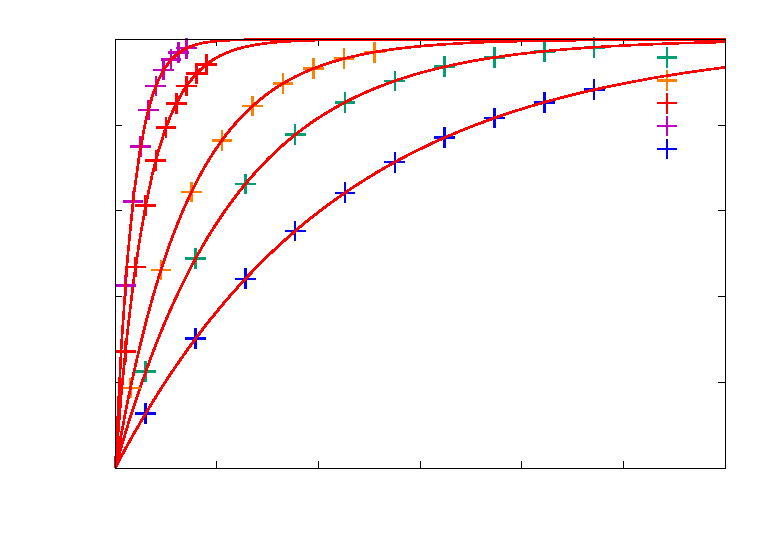
\includegraphics{plots/ManganalleT1}}%
    \gplfronttext
  \end{picture}%
\endgroup

    \caption{Alle Messungen T1Mn2+}
\end{figure}
\begin{figure}[H]
    \centering
    % GNUPLOT: LaTeX picture with Postscript
\begingroup
  % Encoding inside the plot.  In the header of your document, this encoding
  % should to defined, e.g., by using
  % \usepackage[cp1252,<other encodings>]{inputenc}
  \inputencoding{cp1252}%
  \makeatletter
  \providecommand\color[2][]{%
    \GenericError{(gnuplot) \space\space\space\@spaces}{%
      Package color not loaded in conjunction with
      terminal option `colourtext'%
    }{See the gnuplot documentation for explanation.%
    }{Either use 'blacktext' in gnuplot or load the package
      color.sty in LaTeX.}%
    \renewcommand\color[2][]{}%
  }%
  \providecommand\includegraphics[2][]{%
    \GenericError{(gnuplot) \space\space\space\@spaces}{%
      Package graphicx or graphics not loaded%
    }{See the gnuplot documentation for explanation.%
    }{The gnuplot epslatex terminal needs graphicx.sty or graphics.sty.}%
    \renewcommand\includegraphics[2][]{}%
  }%
  \providecommand\rotatebox[2]{#2}%
  \@ifundefined{ifGPcolor}{%
    \newif\ifGPcolor
    \GPcolorfalse
  }{}%
  \@ifundefined{ifGPblacktext}{%
    \newif\ifGPblacktext
    \GPblacktexttrue
  }{}%
  % define a \g@addto@macro without @ in the name:
  \let\gplgaddtomacro\g@addto@macro
  % define empty templates for all commands taking text:
  \gdef\gplbacktext{}%
  \gdef\gplfronttext{}%
  \makeatother
  \ifGPblacktext
    % no textcolor at all
    \def\colorrgb#1{}%
    \def\colorgray#1{}%
  \else
    % gray or color?
    \ifGPcolor
      \def\colorrgb#1{\color[rgb]{#1}}%
      \def\colorgray#1{\color[gray]{#1}}%
      \expandafter\def\csname LTw\endcsname{\color{white}}%
      \expandafter\def\csname LTb\endcsname{\color{black}}%
      \expandafter\def\csname LTa\endcsname{\color{black}}%
      \expandafter\def\csname LT0\endcsname{\color[rgb]{1,0,0}}%
      \expandafter\def\csname LT1\endcsname{\color[rgb]{0,1,0}}%
      \expandafter\def\csname LT2\endcsname{\color[rgb]{0,0,1}}%
      \expandafter\def\csname LT3\endcsname{\color[rgb]{1,0,1}}%
      \expandafter\def\csname LT4\endcsname{\color[rgb]{0,1,1}}%
      \expandafter\def\csname LT5\endcsname{\color[rgb]{1,1,0}}%
      \expandafter\def\csname LT6\endcsname{\color[rgb]{0,0,0}}%
      \expandafter\def\csname LT7\endcsname{\color[rgb]{1,0.3,0}}%
      \expandafter\def\csname LT8\endcsname{\color[rgb]{0.5,0.5,0.5}}%
    \else
      % gray
      \def\colorrgb#1{\color{black}}%
      \def\colorgray#1{\color[gray]{#1}}%
      \expandafter\def\csname LTw\endcsname{\color{white}}%
      \expandafter\def\csname LTb\endcsname{\color{black}}%
      \expandafter\def\csname LTa\endcsname{\color{black}}%
      \expandafter\def\csname LT0\endcsname{\color{black}}%
      \expandafter\def\csname LT1\endcsname{\color{black}}%
      \expandafter\def\csname LT2\endcsname{\color{black}}%
      \expandafter\def\csname LT3\endcsname{\color{black}}%
      \expandafter\def\csname LT4\endcsname{\color{black}}%
      \expandafter\def\csname LT5\endcsname{\color{black}}%
      \expandafter\def\csname LT6\endcsname{\color{black}}%
      \expandafter\def\csname LT7\endcsname{\color{black}}%
      \expandafter\def\csname LT8\endcsname{\color{black}}%
    \fi
  \fi
    \setlength{\unitlength}{0.0500bp}%
    \ifx\gptboxheight\undefined%
      \newlength{\gptboxheight}%
      \newlength{\gptboxwidth}%
      \newsavebox{\gptboxtext}%
    \fi%
    \setlength{\fboxrule}{0.5pt}%
    \setlength{\fboxsep}{1pt}%
\begin{picture}(7200.00,5040.00)%
    \gplgaddtomacro\gplbacktext{%
      \csname LTb\endcsname%%
      \put(814,704){\makebox(0,0)[r]{\strut{}$0$}}%
      \put(814,1527){\makebox(0,0)[r]{\strut{}$0.2$}}%
      \put(814,2350){\makebox(0,0)[r]{\strut{}$0.4$}}%
      \put(814,3173){\makebox(0,0)[r]{\strut{}$0.6$}}%
      \put(814,3996){\makebox(0,0)[r]{\strut{}$0.8$}}%
      \put(814,4819){\makebox(0,0)[r]{\strut{}$1$}}%
      \put(946,484){\makebox(0,0){\strut{}$0$}}%
      \put(1922,484){\makebox(0,0){\strut{}$1000$}}%
      \put(2898,484){\makebox(0,0){\strut{}$2000$}}%
      \put(3875,484){\makebox(0,0){\strut{}$3000$}}%
      \put(4851,484){\makebox(0,0){\strut{}$4000$}}%
      \put(5827,484){\makebox(0,0){\strut{}$5000$}}%
      \put(6803,484){\makebox(0,0){\strut{}$6000$}}%
    }%
    \gplgaddtomacro\gplfronttext{%
      \csname LTb\endcsname%%
      \put(198,2761){\rotatebox{-270}{\makebox(0,0){\strut{}D\"ampfung $\frac{\text{E}}{\text{E}_0}$}}}%
      \put(3874,154){\makebox(0,0){\strut{}Zeit in $\si{\milli \second}$}}%
      \csname LTb\endcsname%%
      \put(5860,4606){\makebox(0,0)[r]{\strut{}$Mn^{2+} \SI{25}{\micro\mole}$}}%
      \csname LTb\endcsname%%
      \put(5860,4386){\makebox(0,0)[r]{\strut{}$Mn^{2+} \SI{100}{\micro\mole}$}}%
      \csname LTb\endcsname%%
      \put(5860,4166){\makebox(0,0)[r]{\strut{}$Mn^{2+} \SI{25}{\micro\mole}$}}%
      \csname LTb\endcsname%%
      \put(5860,3946){\makebox(0,0)[r]{\strut{}$Mn^{2+} \SI{200}{\micro\mole}$}}%
      \csname LTb\endcsname%%
      \put(5860,3726){\makebox(0,0)[r]{\strut{}Wasser}}%
    }%
    \gplbacktext
    \put(0,0){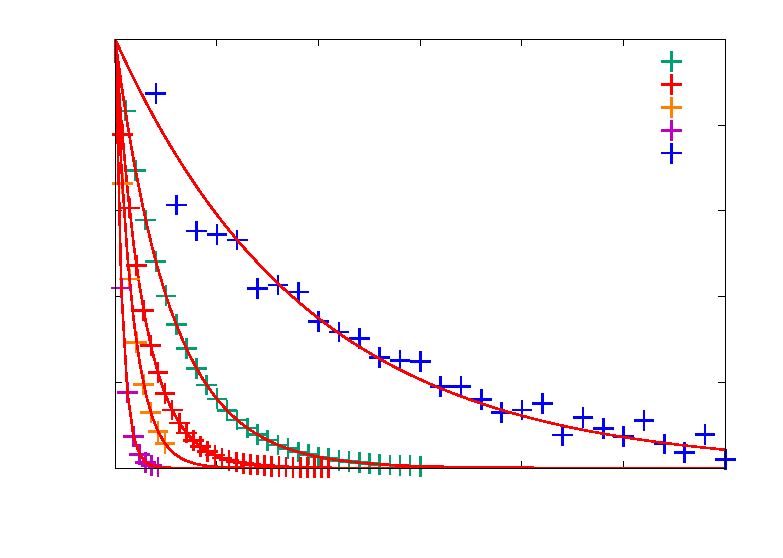
\includegraphics{plots/ManganalleT2}}%
    \gplfronttext
  \end{picture}%
\endgroup

    \caption{Alle Messungen T2MN2+}
\end{figure}

\begin{table}[H]
    \centering]
    \begin{tabular}{lllll}
    \hline
    \multicolumn{1}{|l|}{}            & \multicolumn{1}{l|}{T1}      & \multicolumn{1}{l|}{U(T1)-Fit} & \multicolumn{1}{l|}{T2}      & \multicolumn{1}{l|}{U(T2)-Fit}  \\ \hline
    \multicolumn{1}{|l|}{Cu2    250}  & \multicolumn{1}{l|}{1394,84} & \multicolumn{1}{l|}{0,001055}  & \multicolumn{1}{l|}{1215,51} & \multicolumn{1}{l|}{0,0002529}  \\ \hline
    \multicolumn{1}{|l|}{Cu2    500}  & \multicolumn{1}{l|}{1003,4}  & \multicolumn{1}{l|}{0,0004851} & \multicolumn{1}{l|}{1066,44} & \multicolumn{1}{l|}{0,0002621}  \\ \hline
    \multicolumn{1}{|l|}{Cu2    1000} & \multicolumn{1}{l|}{646,849} & \multicolumn{1}{l|}{71,54}     & \multicolumn{1}{l|}{748,404} & \multicolumn{1}{l|}{0,0001937}  \\ \hline
    \multicolumn{1}{|l|}{Cu2    2000} & \multicolumn{1}{l|}{431,268} & \multicolumn{1}{l|}{0,0002906} & \multicolumn{1}{l|}{341,83}  & \multicolumn{1}{l|}{0,0001228}  \\ \hline
                                      &                              &                                &                              &                                 \\ \hline
    \multicolumn{1}{|l|}{}            & \multicolumn{1}{l|}{T1}      & \multicolumn{1}{l|}{U(T1)-Fit} & \multicolumn{1}{l|}{T2}      & \multicolumn{1}{l|}{U(T2)-Fit}  \\ \hline
    \multicolumn{1}{|l|}{Wasser}      & \multicolumn{1}{l|}{2199,46} & \multicolumn{1}{l|}{0,003027}  & \multicolumn{1}{l|}{1901,06} & \multicolumn{1}{l|}{89,83}      \\ \hline
                                      &                              &                                &                              &                                 \\
                                      &                              &                                &                              &                                 \\ \hline
    \multicolumn{1}{|l|}{}            & \multicolumn{1}{l|}{T1}      & \multicolumn{1}{l|}{U(T1)-Fit} & \multicolumn{1}{l|}{T2}      & \multicolumn{1}{l|}{U(T2)-Fit}  \\ \hline
    \multicolumn{1}{|l|}{Mn 2 25}     & \multicolumn{1}{l|}{1178,28} & \multicolumn{1}{l|}{0,0009801} & \multicolumn{1}{l|}{548,337} & \multicolumn{1}{l|}{0,0001258}  \\ \hline
    \multicolumn{1}{|l|}{Mn 2 50}     & \multicolumn{1}{l|}{725,857} & \multicolumn{1}{l|}{0,0006027} & \multicolumn{1}{l|}{279,858} & \multicolumn{1}{l|}{0,00008179} \\ \hline
    \multicolumn{1}{|l|}{Mn 2 100}    & \multicolumn{1}{l|}{316,085} & \multicolumn{1}{l|}{0,0003079} & \multicolumn{1}{l|}{170,996} & \multicolumn{1}{l|}{0,0001182}  \\ \hline
    \multicolumn{1}{|l|}{Mn 2 200}    & \multicolumn{1}{l|}{180,244} & \multicolumn{1}{l|}{0,0001274} & \multicolumn{1}{l|}{69,1512} & \multicolumn{1}{l|}{0,0000547}  \\ \hline
    \end{tabular}
    \caption{T1- und T2- abhängig von den Stoffen und der Konzentration}
    \end{table}
% GNUPLOT: LaTeX picture with Postscript
\begingroup
  % Encoding inside the plot.  In the header of your document, this encoding
  % should to defined, e.g., by using
  % \usepackage[cp1252,<other encodings>]{inputenc}
  \inputencoding{cp1252}%
  \makeatletter
  \providecommand\color[2][]{%
    \GenericError{(gnuplot) \space\space\space\@spaces}{%
      Package color not loaded in conjunction with
      terminal option `colourtext'%
    }{See the gnuplot documentation for explanation.%
    }{Either use 'blacktext' in gnuplot or load the package
      color.sty in LaTeX.}%
    \renewcommand\color[2][]{}%
  }%
  \providecommand\includegraphics[2][]{%
    \GenericError{(gnuplot) \space\space\space\@spaces}{%
      Package graphicx or graphics not loaded%
    }{See the gnuplot documentation for explanation.%
    }{The gnuplot epslatex terminal needs graphicx.sty or graphics.sty.}%
    \renewcommand\includegraphics[2][]{}%
  }%
  \providecommand\rotatebox[2]{#2}%
  \@ifundefined{ifGPcolor}{%
    \newif\ifGPcolor
    \GPcolorfalse
  }{}%
  \@ifundefined{ifGPblacktext}{%
    \newif\ifGPblacktext
    \GPblacktexttrue
  }{}%
  % define a \g@addto@macro without @ in the name:
  \let\gplgaddtomacro\g@addto@macro
  % define empty templates for all commands taking text:
  \gdef\gplbacktext{}%
  \gdef\gplfronttext{}%
  \makeatother
  \ifGPblacktext
    % no textcolor at all
    \def\colorrgb#1{}%
    \def\colorgray#1{}%
  \else
    % gray or color?
    \ifGPcolor
      \def\colorrgb#1{\color[rgb]{#1}}%
      \def\colorgray#1{\color[gray]{#1}}%
      \expandafter\def\csname LTw\endcsname{\color{white}}%
      \expandafter\def\csname LTb\endcsname{\color{black}}%
      \expandafter\def\csname LTa\endcsname{\color{black}}%
      \expandafter\def\csname LT0\endcsname{\color[rgb]{1,0,0}}%
      \expandafter\def\csname LT1\endcsname{\color[rgb]{0,1,0}}%
      \expandafter\def\csname LT2\endcsname{\color[rgb]{0,0,1}}%
      \expandafter\def\csname LT3\endcsname{\color[rgb]{1,0,1}}%
      \expandafter\def\csname LT4\endcsname{\color[rgb]{0,1,1}}%
      \expandafter\def\csname LT5\endcsname{\color[rgb]{1,1,0}}%
      \expandafter\def\csname LT6\endcsname{\color[rgb]{0,0,0}}%
      \expandafter\def\csname LT7\endcsname{\color[rgb]{1,0.3,0}}%
      \expandafter\def\csname LT8\endcsname{\color[rgb]{0.5,0.5,0.5}}%
    \else
      % gray
      \def\colorrgb#1{\color{black}}%
      \def\colorgray#1{\color[gray]{#1}}%
      \expandafter\def\csname LTw\endcsname{\color{white}}%
      \expandafter\def\csname LTb\endcsname{\color{black}}%
      \expandafter\def\csname LTa\endcsname{\color{black}}%
      \expandafter\def\csname LT0\endcsname{\color{black}}%
      \expandafter\def\csname LT1\endcsname{\color{black}}%
      \expandafter\def\csname LT2\endcsname{\color{black}}%
      \expandafter\def\csname LT3\endcsname{\color{black}}%
      \expandafter\def\csname LT4\endcsname{\color{black}}%
      \expandafter\def\csname LT5\endcsname{\color{black}}%
      \expandafter\def\csname LT6\endcsname{\color{black}}%
      \expandafter\def\csname LT7\endcsname{\color{black}}%
      \expandafter\def\csname LT8\endcsname{\color{black}}%
    \fi
  \fi
    \setlength{\unitlength}{0.0500bp}%
    \ifx\gptboxheight\undefined%
      \newlength{\gptboxheight}%
      \newlength{\gptboxwidth}%
      \newsavebox{\gptboxtext}%
    \fi%
    \setlength{\fboxrule}{0.5pt}%
    \setlength{\fboxsep}{1pt}%
\begin{picture}(7200.00,5040.00)%
    \gplgaddtomacro\gplbacktext{%
      \csname LTb\endcsname%%
      \put(1078,704){\makebox(0,0)[r]{\strut{}$0$}}%
      \put(1078,1292){\makebox(0,0)[r]{\strut{}$5000$}}%
      \put(1078,1880){\makebox(0,0)[r]{\strut{}$10000$}}%
      \put(1078,2468){\makebox(0,0)[r]{\strut{}$15000$}}%
      \put(1078,3055){\makebox(0,0)[r]{\strut{}$20000$}}%
      \put(1078,3643){\makebox(0,0)[r]{\strut{}$25000$}}%
      \put(1078,4231){\makebox(0,0)[r]{\strut{}$30000$}}%
      \put(1078,4819){\makebox(0,0)[r]{\strut{}$35000$}}%
      \put(1385,484){\makebox(0,0){\strut{}$-30$}}%
      \put(2259,484){\makebox(0,0){\strut{}$-20$}}%
      \put(3133,484){\makebox(0,0){\strut{}$-10$}}%
      \put(4007,484){\makebox(0,0){\strut{}$0$}}%
      \put(4880,484){\makebox(0,0){\strut{}$10$}}%
      \put(5754,484){\makebox(0,0){\strut{}$20$}}%
      \put(6628,484){\makebox(0,0){\strut{}$30$}}%
    }%
    \gplgaddtomacro\gplfronttext{%
      \csname LTb\endcsname%%
      \put(198,2761){\rotatebox{-270}{\makebox(0,0){\strut{}Amplitude in $\si{\milli \second}$}}}%
      \put(4006,154){\makebox(0,0){\strut{}Frequenz in $\si{\hertz}$}}%
      \csname LTb\endcsname%%
      \put(5816,4646){\makebox(0,0)[r]{\strut{}1D-MRI Messung, angepasste FOV und Bandbreite  }}%
    }%
    \gplbacktext
    \put(0,0){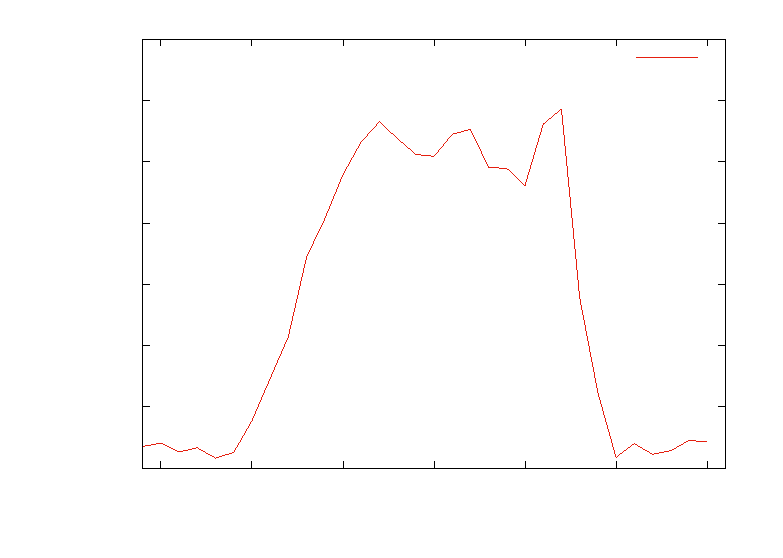
\includegraphics{plots/1DMRI}}%
    \gplfronttext
  \end{picture}%
\endgroup

% !TEX root = main.tex
\section{2D MRI}
\begin{figure}[H]
    \centering
    % GNUPLOT: LaTeX picture with Postscript
\begingroup
  % Encoding inside the plot.  In the header of your document, this encoding
  % should to defined, e.g., by using
  % \usepackage[cp1252,<other encodings>]{inputenc}
  \inputencoding{cp1252}%
  \makeatletter
  \providecommand\color[2][]{%
    \GenericError{(gnuplot) \space\space\space\@spaces}{%
      Package color not loaded in conjunction with
      terminal option `colourtext'%
    }{See the gnuplot documentation for explanation.%
    }{Either use 'blacktext' in gnuplot or load the package
      color.sty in LaTeX.}%
    \renewcommand\color[2][]{}%
  }%
  \providecommand\includegraphics[2][]{%
    \GenericError{(gnuplot) \space\space\space\@spaces}{%
      Package graphicx or graphics not loaded%
    }{See the gnuplot documentation for explanation.%
    }{The gnuplot epslatex terminal needs graphicx.sty or graphics.sty.}%
    \renewcommand\includegraphics[2][]{}%
  }%
  \providecommand\rotatebox[2]{#2}%
  \@ifundefined{ifGPcolor}{%
    \newif\ifGPcolor
    \GPcolorfalse
  }{}%
  \@ifundefined{ifGPblacktext}{%
    \newif\ifGPblacktext
    \GPblacktexttrue
  }{}%
  % define a \g@addto@macro without @ in the name:
  \let\gplgaddtomacro\g@addto@macro
  % define empty templates for all commands taking text:
  \gdef\gplbacktext{}%
  \gdef\gplfronttext{}%
  \makeatother
  \ifGPblacktext
    % no textcolor at all
    \def\colorrgb#1{}%
    \def\colorgray#1{}%
  \else
    % gray or color?
    \ifGPcolor
      \def\colorrgb#1{\color[rgb]{#1}}%
      \def\colorgray#1{\color[gray]{#1}}%
      \expandafter\def\csname LTw\endcsname{\color{white}}%
      \expandafter\def\csname LTb\endcsname{\color{black}}%
      \expandafter\def\csname LTa\endcsname{\color{black}}%
      \expandafter\def\csname LT0\endcsname{\color[rgb]{1,0,0}}%
      \expandafter\def\csname LT1\endcsname{\color[rgb]{0,1,0}}%
      \expandafter\def\csname LT2\endcsname{\color[rgb]{0,0,1}}%
      \expandafter\def\csname LT3\endcsname{\color[rgb]{1,0,1}}%
      \expandafter\def\csname LT4\endcsname{\color[rgb]{0,1,1}}%
      \expandafter\def\csname LT5\endcsname{\color[rgb]{1,1,0}}%
      \expandafter\def\csname LT6\endcsname{\color[rgb]{0,0,0}}%
      \expandafter\def\csname LT7\endcsname{\color[rgb]{1,0.3,0}}%
      \expandafter\def\csname LT8\endcsname{\color[rgb]{0.5,0.5,0.5}}%
    \else
      % gray
      \def\colorrgb#1{\color{black}}%
      \def\colorgray#1{\color[gray]{#1}}%
      \expandafter\def\csname LTw\endcsname{\color{white}}%
      \expandafter\def\csname LTb\endcsname{\color{black}}%
      \expandafter\def\csname LTa\endcsname{\color{black}}%
      \expandafter\def\csname LT0\endcsname{\color{black}}%
      \expandafter\def\csname LT1\endcsname{\color{black}}%
      \expandafter\def\csname LT2\endcsname{\color{black}}%
      \expandafter\def\csname LT3\endcsname{\color{black}}%
      \expandafter\def\csname LT4\endcsname{\color{black}}%
      \expandafter\def\csname LT5\endcsname{\color{black}}%
      \expandafter\def\csname LT6\endcsname{\color{black}}%
      \expandafter\def\csname LT7\endcsname{\color{black}}%
      \expandafter\def\csname LT8\endcsname{\color{black}}%
    \fi
  \fi
    \setlength{\unitlength}{0.0500bp}%
    \ifx\gptboxheight\undefined%
      \newlength{\gptboxheight}%
      \newlength{\gptboxwidth}%
      \newsavebox{\gptboxtext}%
    \fi%
    \setlength{\fboxrule}{0.5pt}%
    \setlength{\fboxsep}{1pt}%
\begin{picture}(7200.00,5040.00)%
    \gplgaddtomacro\gplbacktext{%
      \csname LTb\endcsname%%
      \put(682,704){\makebox(0,0)[r]{\strut{}$0$}}%
      \put(682,1527){\makebox(0,0)[r]{\strut{}$2$}}%
      \put(682,2350){\makebox(0,0)[r]{\strut{}$4$}}%
      \put(682,3173){\makebox(0,0)[r]{\strut{}$6$}}%
      \put(682,3996){\makebox(0,0)[r]{\strut{}$8$}}%
      \put(682,4819){\makebox(0,0)[r]{\strut{}$10$}}%
      \put(814,484){\makebox(0,0){\strut{}$1820$}}%
      \put(1563,484){\makebox(0,0){\strut{}$1825$}}%
      \put(2311,484){\makebox(0,0){\strut{}$1830$}}%
      \put(3060,484){\makebox(0,0){\strut{}$1835$}}%
      \put(3809,484){\makebox(0,0){\strut{}$1840$}}%
      \put(4557,484){\makebox(0,0){\strut{}$1845$}}%
      \put(5306,484){\makebox(0,0){\strut{}$1850$}}%
      \put(6054,484){\makebox(0,0){\strut{}$1855$}}%
      \put(6803,484){\makebox(0,0){\strut{}$1860$}}%
    }%
    \gplgaddtomacro\gplfronttext{%
      \csname LTb\endcsname%%
      \put(198,2761){\rotatebox{-270}{\makebox(0,0){\strut{}Amplitude in $\si{\milli \second}$}}}%
      \put(3808,154){\makebox(0,0){\strut{}Frequenz in $\si{\hertz}$}}%
      \csname LTb\endcsname%%
      \put(5816,4646){\makebox(0,0)[r]{\strut{}Puls and Collect Experiment zur Feinjustierung der 2D Messung}}%
    }%
    \gplbacktext
    \put(0,0){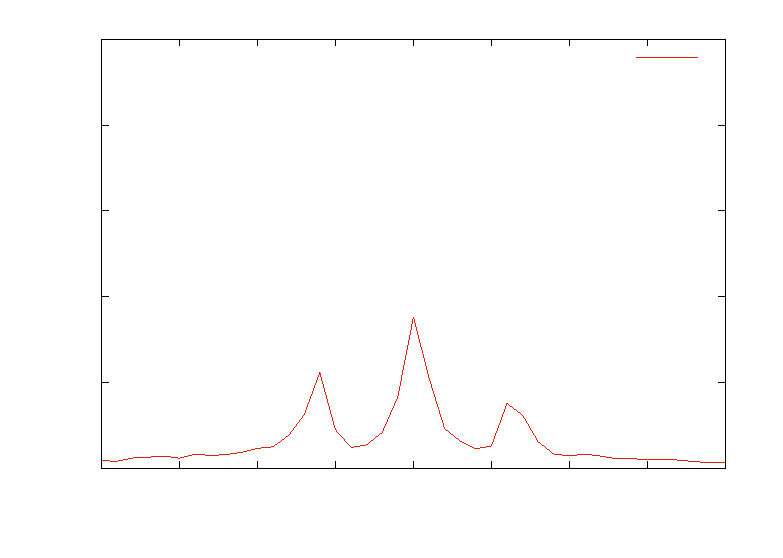
\includegraphics{plots/Tunensignalpulsandcollect}}%
    \gplfronttext
  \end{picture}%
\endgroup

    \caption{Zum tunen benutzte Daten des Puls and collect Experiments; Man soll noch die Integrale berechnen der einzelnen Peaks(aus den Integralen bekommt man dann das Verhältnuis von 1:2:3:3:2:1 oder so halt); Diese Peaks fitten bzw den abstand der Maximas berechnen=< daraus dann die Kopplungaskostante}
\end{figure}

\begin{figure}[H]
    \centering
    % GNUPLOT: LaTeX picture with Postscript
\begingroup
  % Encoding inside the plot.  In the header of your document, this encoding
  % should to defined, e.g., by using
  % \usepackage[cp1252,<other encodings>]{inputenc}
  \inputencoding{cp1252}%
  \makeatletter
  \providecommand\color[2][]{%
    \GenericError{(gnuplot) \space\space\space\@spaces}{%
      Package color not loaded in conjunction with
      terminal option `colourtext'%
    }{See the gnuplot documentation for explanation.%
    }{Either use 'blacktext' in gnuplot or load the package
      color.sty in LaTeX.}%
    \renewcommand\color[2][]{}%
  }%
  \providecommand\includegraphics[2][]{%
    \GenericError{(gnuplot) \space\space\space\@spaces}{%
      Package graphicx or graphics not loaded%
    }{See the gnuplot documentation for explanation.%
    }{The gnuplot epslatex terminal needs graphicx.sty or graphics.sty.}%
    \renewcommand\includegraphics[2][]{}%
  }%
  \providecommand\rotatebox[2]{#2}%
  \@ifundefined{ifGPcolor}{%
    \newif\ifGPcolor
    \GPcolorfalse
  }{}%
  \@ifundefined{ifGPblacktext}{%
    \newif\ifGPblacktext
    \GPblacktexttrue
  }{}%
  % define a \g@addto@macro without @ in the name:
  \let\gplgaddtomacro\g@addto@macro
  % define empty templates for all commands taking text:
  \gdef\gplbacktext{}%
  \gdef\gplfronttext{}%
  \makeatother
  \ifGPblacktext
    % no textcolor at all
    \def\colorrgb#1{}%
    \def\colorgray#1{}%
  \else
    % gray or color?
    \ifGPcolor
      \def\colorrgb#1{\color[rgb]{#1}}%
      \def\colorgray#1{\color[gray]{#1}}%
      \expandafter\def\csname LTw\endcsname{\color{white}}%
      \expandafter\def\csname LTb\endcsname{\color{black}}%
      \expandafter\def\csname LTa\endcsname{\color{black}}%
      \expandafter\def\csname LT0\endcsname{\color[rgb]{1,0,0}}%
      \expandafter\def\csname LT1\endcsname{\color[rgb]{0,1,0}}%
      \expandafter\def\csname LT2\endcsname{\color[rgb]{0,0,1}}%
      \expandafter\def\csname LT3\endcsname{\color[rgb]{1,0,1}}%
      \expandafter\def\csname LT4\endcsname{\color[rgb]{0,1,1}}%
      \expandafter\def\csname LT5\endcsname{\color[rgb]{1,1,0}}%
      \expandafter\def\csname LT6\endcsname{\color[rgb]{0,0,0}}%
      \expandafter\def\csname LT7\endcsname{\color[rgb]{1,0.3,0}}%
      \expandafter\def\csname LT8\endcsname{\color[rgb]{0.5,0.5,0.5}}%
    \else
      % gray
      \def\colorrgb#1{\color{black}}%
      \def\colorgray#1{\color[gray]{#1}}%
      \expandafter\def\csname LTw\endcsname{\color{white}}%
      \expandafter\def\csname LTb\endcsname{\color{black}}%
      \expandafter\def\csname LTa\endcsname{\color{black}}%
      \expandafter\def\csname LT0\endcsname{\color{black}}%
      \expandafter\def\csname LT1\endcsname{\color{black}}%
      \expandafter\def\csname LT2\endcsname{\color{black}}%
      \expandafter\def\csname LT3\endcsname{\color{black}}%
      \expandafter\def\csname LT4\endcsname{\color{black}}%
      \expandafter\def\csname LT5\endcsname{\color{black}}%
      \expandafter\def\csname LT6\endcsname{\color{black}}%
      \expandafter\def\csname LT7\endcsname{\color{black}}%
      \expandafter\def\csname LT8\endcsname{\color{black}}%
    \fi
  \fi
    \setlength{\unitlength}{0.0500bp}%
    \ifx\gptboxheight\undefined%
      \newlength{\gptboxheight}%
      \newlength{\gptboxwidth}%
      \newsavebox{\gptboxtext}%
    \fi%
    \setlength{\fboxrule}{0.5pt}%
    \setlength{\fboxsep}{1pt}%
\begin{picture}(7200.00,5040.00)%
    \gplgaddtomacro\gplbacktext{%
    }%
    \gplgaddtomacro\gplfronttext{%
      \csname LTb\endcsname%%
      \put(936,688){\makebox(0,0){\strut{}$0$}}%
      \put(1824,688){\makebox(0,0){\strut{}$20$}}%
      \put(2712,688){\makebox(0,0){\strut{}$40$}}%
      \put(3600,688){\makebox(0,0){\strut{}$60$}}%
      \put(4488,688){\makebox(0,0){\strut{}$80$}}%
      \put(5376,688){\makebox(0,0){\strut{}$100$}}%
      \put(6264,688){\makebox(0,0){\strut{}$120$}}%
      \put(3600,358){\makebox(0,0){\strut{}Y in $\si{\milli \meter}$}}%
      \put(700,938){\makebox(0,0)[r]{\strut{}$0$}}%
      \put(700,1502){\makebox(0,0)[r]{\strut{}$20$}}%
      \put(700,2066){\makebox(0,0)[r]{\strut{}$40$}}%
      \put(700,2630){\makebox(0,0)[r]{\strut{}$60$}}%
      \put(700,3194){\makebox(0,0)[r]{\strut{}$80$}}%
      \put(700,3758){\makebox(0,0)[r]{\strut{}$100$}}%
      \put(700,4322){\makebox(0,0)[r]{\strut{}$120$}}%
      \put(238,2630){\rotatebox{-270}{\makebox(0,0){\strut{}Z in $\si{\milli \meter}$}}}%
      \put(6795,938){\makebox(0,0)[l]{\strut{}$0$}}%
      \put(6795,1421){\makebox(0,0)[l]{\strut{}$5000$}}%
      \put(6795,1904){\makebox(0,0)[l]{\strut{}$10000$}}%
      \put(6795,2388){\makebox(0,0)[l]{\strut{}$15000$}}%
      \put(6795,2871){\makebox(0,0)[l]{\strut{}$20000$}}%
      \put(6795,3355){\makebox(0,0)[l]{\strut{}$25000$}}%
      \put(6795,3838){\makebox(0,0)[l]{\strut{}$30000$}}%
      \put(6795,4322){\makebox(0,0)[l]{\strut{}$35000$}}%
    }%
    \gplbacktext
    \put(0,0){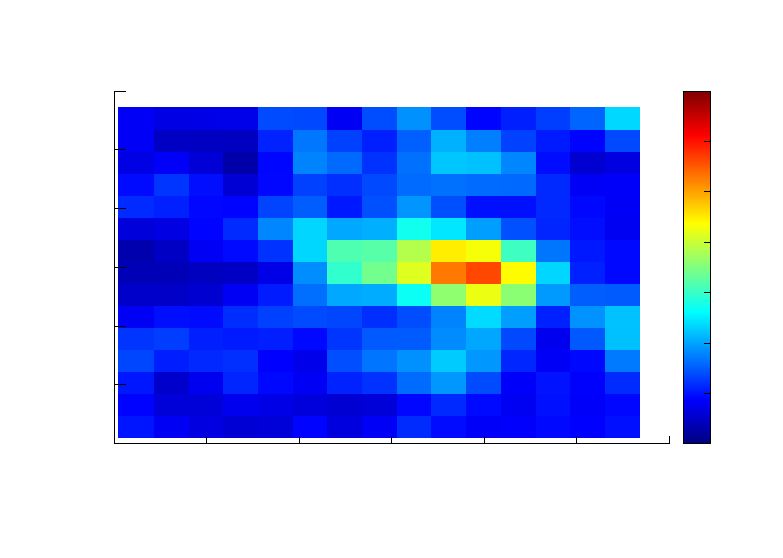
\includegraphics{plots/2DMRI600}}%
    \gplfronttext
  \end{picture}%
\endgroup

    \caption{2D MRI mit T1 $\SI{600}{\milli\second}$}
\end{figure}

\begin{figure}[H]
    \centering
    % GNUPLOT: LaTeX picture with Postscript
\begingroup
  % Encoding inside the plot.  In the header of your document, this encoding
  % should to defined, e.g., by using
  % \usepackage[cp1252,<other encodings>]{inputenc}
  \inputencoding{cp1252}%
  \makeatletter
  \providecommand\color[2][]{%
    \GenericError{(gnuplot) \space\space\space\@spaces}{%
      Package color not loaded in conjunction with
      terminal option `colourtext'%
    }{See the gnuplot documentation for explanation.%
    }{Either use 'blacktext' in gnuplot or load the package
      color.sty in LaTeX.}%
    \renewcommand\color[2][]{}%
  }%
  \providecommand\includegraphics[2][]{%
    \GenericError{(gnuplot) \space\space\space\@spaces}{%
      Package graphicx or graphics not loaded%
    }{See the gnuplot documentation for explanation.%
    }{The gnuplot epslatex terminal needs graphicx.sty or graphics.sty.}%
    \renewcommand\includegraphics[2][]{}%
  }%
  \providecommand\rotatebox[2]{#2}%
  \@ifundefined{ifGPcolor}{%
    \newif\ifGPcolor
    \GPcolorfalse
  }{}%
  \@ifundefined{ifGPblacktext}{%
    \newif\ifGPblacktext
    \GPblacktexttrue
  }{}%
  % define a \g@addto@macro without @ in the name:
  \let\gplgaddtomacro\g@addto@macro
  % define empty templates for all commands taking text:
  \gdef\gplbacktext{}%
  \gdef\gplfronttext{}%
  \makeatother
  \ifGPblacktext
    % no textcolor at all
    \def\colorrgb#1{}%
    \def\colorgray#1{}%
  \else
    % gray or color?
    \ifGPcolor
      \def\colorrgb#1{\color[rgb]{#1}}%
      \def\colorgray#1{\color[gray]{#1}}%
      \expandafter\def\csname LTw\endcsname{\color{white}}%
      \expandafter\def\csname LTb\endcsname{\color{black}}%
      \expandafter\def\csname LTa\endcsname{\color{black}}%
      \expandafter\def\csname LT0\endcsname{\color[rgb]{1,0,0}}%
      \expandafter\def\csname LT1\endcsname{\color[rgb]{0,1,0}}%
      \expandafter\def\csname LT2\endcsname{\color[rgb]{0,0,1}}%
      \expandafter\def\csname LT3\endcsname{\color[rgb]{1,0,1}}%
      \expandafter\def\csname LT4\endcsname{\color[rgb]{0,1,1}}%
      \expandafter\def\csname LT5\endcsname{\color[rgb]{1,1,0}}%
      \expandafter\def\csname LT6\endcsname{\color[rgb]{0,0,0}}%
      \expandafter\def\csname LT7\endcsname{\color[rgb]{1,0.3,0}}%
      \expandafter\def\csname LT8\endcsname{\color[rgb]{0.5,0.5,0.5}}%
    \else
      % gray
      \def\colorrgb#1{\color{black}}%
      \def\colorgray#1{\color[gray]{#1}}%
      \expandafter\def\csname LTw\endcsname{\color{white}}%
      \expandafter\def\csname LTb\endcsname{\color{black}}%
      \expandafter\def\csname LTa\endcsname{\color{black}}%
      \expandafter\def\csname LT0\endcsname{\color{black}}%
      \expandafter\def\csname LT1\endcsname{\color{black}}%
      \expandafter\def\csname LT2\endcsname{\color{black}}%
      \expandafter\def\csname LT3\endcsname{\color{black}}%
      \expandafter\def\csname LT4\endcsname{\color{black}}%
      \expandafter\def\csname LT5\endcsname{\color{black}}%
      \expandafter\def\csname LT6\endcsname{\color{black}}%
      \expandafter\def\csname LT7\endcsname{\color{black}}%
      \expandafter\def\csname LT8\endcsname{\color{black}}%
    \fi
  \fi
    \setlength{\unitlength}{0.0500bp}%
    \ifx\gptboxheight\undefined%
      \newlength{\gptboxheight}%
      \newlength{\gptboxwidth}%
      \newsavebox{\gptboxtext}%
    \fi%
    \setlength{\fboxrule}{0.5pt}%
    \setlength{\fboxsep}{1pt}%
\begin{picture}(7200.00,5040.00)%
    \gplgaddtomacro\gplbacktext{%
    }%
    \gplgaddtomacro\gplfronttext{%
      \csname LTb\endcsname%%
      \put(936,688){\makebox(0,0){\strut{}$0$}}%
      \put(1824,688){\makebox(0,0){\strut{}$20$}}%
      \put(2712,688){\makebox(0,0){\strut{}$40$}}%
      \put(3600,688){\makebox(0,0){\strut{}$60$}}%
      \put(4488,688){\makebox(0,0){\strut{}$80$}}%
      \put(5376,688){\makebox(0,0){\strut{}$100$}}%
      \put(6264,688){\makebox(0,0){\strut{}$120$}}%
      \put(3600,358){\makebox(0,0){\strut{}Y in $\si{\milli \meter}$}}%
      \put(700,938){\makebox(0,0)[r]{\strut{}$0$}}%
      \put(700,1502){\makebox(0,0)[r]{\strut{}$20$}}%
      \put(700,2066){\makebox(0,0)[r]{\strut{}$40$}}%
      \put(700,2630){\makebox(0,0)[r]{\strut{}$60$}}%
      \put(700,3194){\makebox(0,0)[r]{\strut{}$80$}}%
      \put(700,3758){\makebox(0,0)[r]{\strut{}$100$}}%
      \put(700,4322){\makebox(0,0)[r]{\strut{}$120$}}%
      \put(238,2630){\rotatebox{-270}{\makebox(0,0){\strut{}Z in $\si{\milli \meter}$}}}%
      \put(6795,938){\makebox(0,0)[l]{\strut{}$0$}}%
      \put(6795,1502){\makebox(0,0)[l]{\strut{}$10000$}}%
      \put(6795,2066){\makebox(0,0)[l]{\strut{}$20000$}}%
      \put(6795,2630){\makebox(0,0)[l]{\strut{}$30000$}}%
      \put(6795,3194){\makebox(0,0)[l]{\strut{}$40000$}}%
      \put(6795,3758){\makebox(0,0)[l]{\strut{}$50000$}}%
      \put(6795,4322){\makebox(0,0)[l]{\strut{}$60000$}}%
    }%
    \gplbacktext
    \put(0,0){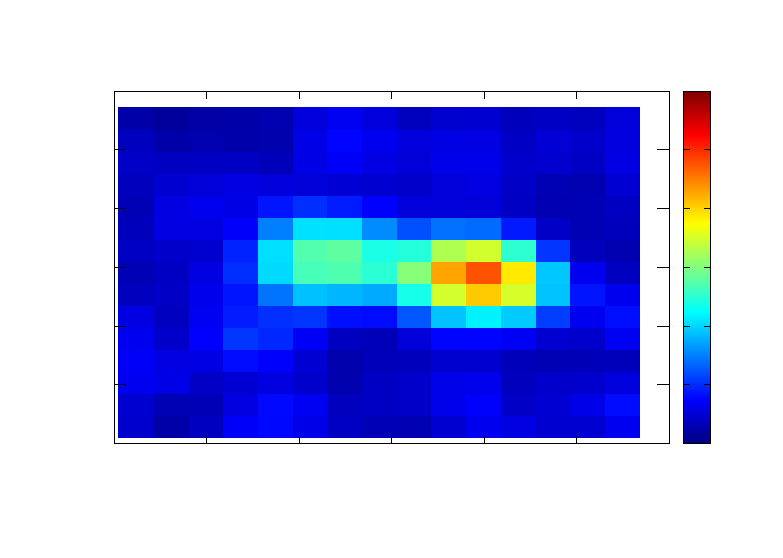
\includegraphics{plots/2DMRI1300}}%
    \gplfronttext
  \end{picture}%
\endgroup

    \caption{2D MRI mit T1 $\SI{1300}{\milli\second}$}
\end{figure}
\begin{figure}[H]
    \centering
    % GNUPLOT: LaTeX picture with Postscript
\begingroup
  % Encoding inside the plot.  In the header of your document, this encoding
  % should to defined, e.g., by using
  % \usepackage[cp1252,<other encodings>]{inputenc}
  \inputencoding{cp1252}%
  \makeatletter
  \providecommand\color[2][]{%
    \GenericError{(gnuplot) \space\space\space\@spaces}{%
      Package color not loaded in conjunction with
      terminal option `colourtext'%
    }{See the gnuplot documentation for explanation.%
    }{Either use 'blacktext' in gnuplot or load the package
      color.sty in LaTeX.}%
    \renewcommand\color[2][]{}%
  }%
  \providecommand\includegraphics[2][]{%
    \GenericError{(gnuplot) \space\space\space\@spaces}{%
      Package graphicx or graphics not loaded%
    }{See the gnuplot documentation for explanation.%
    }{The gnuplot epslatex terminal needs graphicx.sty or graphics.sty.}%
    \renewcommand\includegraphics[2][]{}%
  }%
  \providecommand\rotatebox[2]{#2}%
  \@ifundefined{ifGPcolor}{%
    \newif\ifGPcolor
    \GPcolorfalse
  }{}%
  \@ifundefined{ifGPblacktext}{%
    \newif\ifGPblacktext
    \GPblacktexttrue
  }{}%
  % define a \g@addto@macro without @ in the name:
  \let\gplgaddtomacro\g@addto@macro
  % define empty templates for all commands taking text:
  \gdef\gplbacktext{}%
  \gdef\gplfronttext{}%
  \makeatother
  \ifGPblacktext
    % no textcolor at all
    \def\colorrgb#1{}%
    \def\colorgray#1{}%
  \else
    % gray or color?
    \ifGPcolor
      \def\colorrgb#1{\color[rgb]{#1}}%
      \def\colorgray#1{\color[gray]{#1}}%
      \expandafter\def\csname LTw\endcsname{\color{white}}%
      \expandafter\def\csname LTb\endcsname{\color{black}}%
      \expandafter\def\csname LTa\endcsname{\color{black}}%
      \expandafter\def\csname LT0\endcsname{\color[rgb]{1,0,0}}%
      \expandafter\def\csname LT1\endcsname{\color[rgb]{0,1,0}}%
      \expandafter\def\csname LT2\endcsname{\color[rgb]{0,0,1}}%
      \expandafter\def\csname LT3\endcsname{\color[rgb]{1,0,1}}%
      \expandafter\def\csname LT4\endcsname{\color[rgb]{0,1,1}}%
      \expandafter\def\csname LT5\endcsname{\color[rgb]{1,1,0}}%
      \expandafter\def\csname LT6\endcsname{\color[rgb]{0,0,0}}%
      \expandafter\def\csname LT7\endcsname{\color[rgb]{1,0.3,0}}%
      \expandafter\def\csname LT8\endcsname{\color[rgb]{0.5,0.5,0.5}}%
    \else
      % gray
      \def\colorrgb#1{\color{black}}%
      \def\colorgray#1{\color[gray]{#1}}%
      \expandafter\def\csname LTw\endcsname{\color{white}}%
      \expandafter\def\csname LTb\endcsname{\color{black}}%
      \expandafter\def\csname LTa\endcsname{\color{black}}%
      \expandafter\def\csname LT0\endcsname{\color{black}}%
      \expandafter\def\csname LT1\endcsname{\color{black}}%
      \expandafter\def\csname LT2\endcsname{\color{black}}%
      \expandafter\def\csname LT3\endcsname{\color{black}}%
      \expandafter\def\csname LT4\endcsname{\color{black}}%
      \expandafter\def\csname LT5\endcsname{\color{black}}%
      \expandafter\def\csname LT6\endcsname{\color{black}}%
      \expandafter\def\csname LT7\endcsname{\color{black}}%
      \expandafter\def\csname LT8\endcsname{\color{black}}%
    \fi
  \fi
    \setlength{\unitlength}{0.0500bp}%
    \ifx\gptboxheight\undefined%
      \newlength{\gptboxheight}%
      \newlength{\gptboxwidth}%
      \newsavebox{\gptboxtext}%
    \fi%
    \setlength{\fboxrule}{0.5pt}%
    \setlength{\fboxsep}{1pt}%
\begin{picture}(7200.00,5040.00)%
    \gplgaddtomacro\gplbacktext{%
    }%
    \gplgaddtomacro\gplfronttext{%
      \csname LTb\endcsname%%
      \put(936,688){\makebox(0,0){\strut{}$0$}}%
      \put(1824,688){\makebox(0,0){\strut{}$20$}}%
      \put(2712,688){\makebox(0,0){\strut{}$40$}}%
      \put(3600,688){\makebox(0,0){\strut{}$60$}}%
      \put(4488,688){\makebox(0,0){\strut{}$80$}}%
      \put(5376,688){\makebox(0,0){\strut{}$100$}}%
      \put(6264,688){\makebox(0,0){\strut{}$120$}}%
      \put(3600,358){\makebox(0,0){\strut{}Y in $\si{\milli \meter}$}}%
      \put(700,938){\makebox(0,0)[r]{\strut{}$0$}}%
      \put(700,1502){\makebox(0,0)[r]{\strut{}$20$}}%
      \put(700,2066){\makebox(0,0)[r]{\strut{}$40$}}%
      \put(700,2630){\makebox(0,0)[r]{\strut{}$60$}}%
      \put(700,3194){\makebox(0,0)[r]{\strut{}$80$}}%
      \put(700,3758){\makebox(0,0)[r]{\strut{}$100$}}%
      \put(700,4322){\makebox(0,0)[r]{\strut{}$120$}}%
      \put(238,2630){\rotatebox{-270}{\makebox(0,0){\strut{}Z in $\si{\milli \meter}$}}}%
      \put(6795,938){\makebox(0,0)[l]{\strut{}$0$}}%
      \put(6795,1502){\makebox(0,0)[l]{\strut{}$10000$}}%
      \put(6795,2066){\makebox(0,0)[l]{\strut{}$20000$}}%
      \put(6795,2630){\makebox(0,0)[l]{\strut{}$30000$}}%
      \put(6795,3194){\makebox(0,0)[l]{\strut{}$40000$}}%
      \put(6795,3758){\makebox(0,0)[l]{\strut{}$50000$}}%
      \put(6795,4322){\makebox(0,0)[l]{\strut{}$60000$}}%
    }%
    \gplbacktext
    \put(0,0){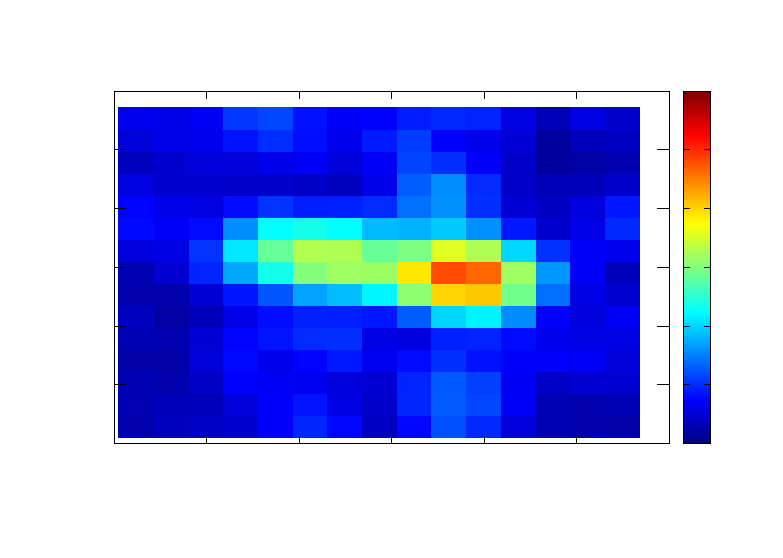
\includegraphics{plots/2DMRI2100}}%
    \gplfronttext
  \end{picture}%
\endgroup

    \caption{2D MRI mit T1 $\SI{2100}{\milli\second}$}
\end{figure}
\begin{figure}[H]
    \centering
    % GNUPLOT: LaTeX picture with Postscript
\begingroup
  % Encoding inside the plot.  In the header of your document, this encoding
  % should to defined, e.g., by using
  % \usepackage[cp1252,<other encodings>]{inputenc}
  \inputencoding{cp1252}%
  \makeatletter
  \providecommand\color[2][]{%
    \GenericError{(gnuplot) \space\space\space\@spaces}{%
      Package color not loaded in conjunction with
      terminal option `colourtext'%
    }{See the gnuplot documentation for explanation.%
    }{Either use 'blacktext' in gnuplot or load the package
      color.sty in LaTeX.}%
    \renewcommand\color[2][]{}%
  }%
  \providecommand\includegraphics[2][]{%
    \GenericError{(gnuplot) \space\space\space\@spaces}{%
      Package graphicx or graphics not loaded%
    }{See the gnuplot documentation for explanation.%
    }{The gnuplot epslatex terminal needs graphicx.sty or graphics.sty.}%
    \renewcommand\includegraphics[2][]{}%
  }%
  \providecommand\rotatebox[2]{#2}%
  \@ifundefined{ifGPcolor}{%
    \newif\ifGPcolor
    \GPcolorfalse
  }{}%
  \@ifundefined{ifGPblacktext}{%
    \newif\ifGPblacktext
    \GPblacktexttrue
  }{}%
  % define a \g@addto@macro without @ in the name:
  \let\gplgaddtomacro\g@addto@macro
  % define empty templates for all commands taking text:
  \gdef\gplbacktext{}%
  \gdef\gplfronttext{}%
  \makeatother
  \ifGPblacktext
    % no textcolor at all
    \def\colorrgb#1{}%
    \def\colorgray#1{}%
  \else
    % gray or color?
    \ifGPcolor
      \def\colorrgb#1{\color[rgb]{#1}}%
      \def\colorgray#1{\color[gray]{#1}}%
      \expandafter\def\csname LTw\endcsname{\color{white}}%
      \expandafter\def\csname LTb\endcsname{\color{black}}%
      \expandafter\def\csname LTa\endcsname{\color{black}}%
      \expandafter\def\csname LT0\endcsname{\color[rgb]{1,0,0}}%
      \expandafter\def\csname LT1\endcsname{\color[rgb]{0,1,0}}%
      \expandafter\def\csname LT2\endcsname{\color[rgb]{0,0,1}}%
      \expandafter\def\csname LT3\endcsname{\color[rgb]{1,0,1}}%
      \expandafter\def\csname LT4\endcsname{\color[rgb]{0,1,1}}%
      \expandafter\def\csname LT5\endcsname{\color[rgb]{1,1,0}}%
      \expandafter\def\csname LT6\endcsname{\color[rgb]{0,0,0}}%
      \expandafter\def\csname LT7\endcsname{\color[rgb]{1,0.3,0}}%
      \expandafter\def\csname LT8\endcsname{\color[rgb]{0.5,0.5,0.5}}%
    \else
      % gray
      \def\colorrgb#1{\color{black}}%
      \def\colorgray#1{\color[gray]{#1}}%
      \expandafter\def\csname LTw\endcsname{\color{white}}%
      \expandafter\def\csname LTb\endcsname{\color{black}}%
      \expandafter\def\csname LTa\endcsname{\color{black}}%
      \expandafter\def\csname LT0\endcsname{\color{black}}%
      \expandafter\def\csname LT1\endcsname{\color{black}}%
      \expandafter\def\csname LT2\endcsname{\color{black}}%
      \expandafter\def\csname LT3\endcsname{\color{black}}%
      \expandafter\def\csname LT4\endcsname{\color{black}}%
      \expandafter\def\csname LT5\endcsname{\color{black}}%
      \expandafter\def\csname LT6\endcsname{\color{black}}%
      \expandafter\def\csname LT7\endcsname{\color{black}}%
      \expandafter\def\csname LT8\endcsname{\color{black}}%
    \fi
  \fi
    \setlength{\unitlength}{0.0500bp}%
    \ifx\gptboxheight\undefined%
      \newlength{\gptboxheight}%
      \newlength{\gptboxwidth}%
      \newsavebox{\gptboxtext}%
    \fi%
    \setlength{\fboxrule}{0.5pt}%
    \setlength{\fboxsep}{1pt}%
\begin{picture}(7200.00,5040.00)%
    \gplgaddtomacro\gplbacktext{%
    }%
    \gplgaddtomacro\gplfronttext{%
      \csname LTb\endcsname%%
      \put(936,688){\makebox(0,0){\strut{}$0$}}%
      \put(1824,688){\makebox(0,0){\strut{}$20$}}%
      \put(2712,688){\makebox(0,0){\strut{}$40$}}%
      \put(3600,688){\makebox(0,0){\strut{}$60$}}%
      \put(4488,688){\makebox(0,0){\strut{}$80$}}%
      \put(5376,688){\makebox(0,0){\strut{}$100$}}%
      \put(6264,688){\makebox(0,0){\strut{}$120$}}%
      \put(3600,358){\makebox(0,0){\strut{}Y in $\si{\milli \meter}$}}%
      \put(700,938){\makebox(0,0)[r]{\strut{}$0$}}%
      \put(700,1502){\makebox(0,0)[r]{\strut{}$20$}}%
      \put(700,2066){\makebox(0,0)[r]{\strut{}$40$}}%
      \put(700,2630){\makebox(0,0)[r]{\strut{}$60$}}%
      \put(700,3194){\makebox(0,0)[r]{\strut{}$80$}}%
      \put(700,3758){\makebox(0,0)[r]{\strut{}$100$}}%
      \put(700,4322){\makebox(0,0)[r]{\strut{}$120$}}%
      \put(238,2630){\rotatebox{-270}{\makebox(0,0){\strut{}Z in $\si{\milli \meter}$}}}%
      \put(6795,938){\makebox(0,0)[l]{\strut{}$0$}}%
      \put(6795,1502){\makebox(0,0)[l]{\strut{}$10000$}}%
      \put(6795,2066){\makebox(0,0)[l]{\strut{}$20000$}}%
      \put(6795,2630){\makebox(0,0)[l]{\strut{}$30000$}}%
      \put(6795,3194){\makebox(0,0)[l]{\strut{}$40000$}}%
      \put(6795,3758){\makebox(0,0)[l]{\strut{}$50000$}}%
      \put(6795,4322){\makebox(0,0)[l]{\strut{}$60000$}}%
    }%
    \gplbacktext
    \put(0,0){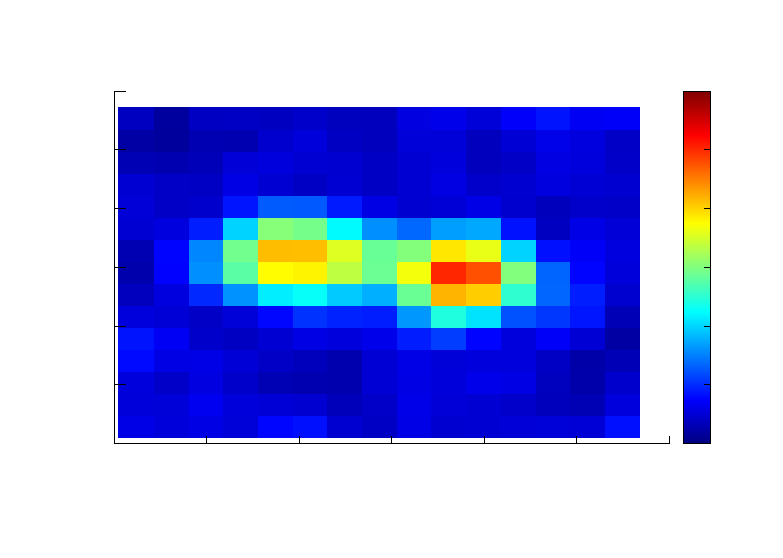
\includegraphics{plots/2DMRI2800}}%
    \gplfronttext
  \end{picture}%
\endgroup

    \caption{2D MRI mit T1 $\SI{2800}{\milli\second}$}
\end{figure}

\begin{figure}[H]
    \centering
    % GNUPLOT: LaTeX picture with Postscript
\begingroup
  % Encoding inside the plot.  In the header of your document, this encoding
  % should to defined, e.g., by using
  % \usepackage[cp1252,<other encodings>]{inputenc}
  \inputencoding{cp1252}%
  \makeatletter
  \providecommand\color[2][]{%
    \GenericError{(gnuplot) \space\space\space\@spaces}{%
      Package color not loaded in conjunction with
      terminal option `colourtext'%
    }{See the gnuplot documentation for explanation.%
    }{Either use 'blacktext' in gnuplot or load the package
      color.sty in LaTeX.}%
    \renewcommand\color[2][]{}%
  }%
  \providecommand\includegraphics[2][]{%
    \GenericError{(gnuplot) \space\space\space\@spaces}{%
      Package graphicx or graphics not loaded%
    }{See the gnuplot documentation for explanation.%
    }{The gnuplot epslatex terminal needs graphicx.sty or graphics.sty.}%
    \renewcommand\includegraphics[2][]{}%
  }%
  \providecommand\rotatebox[2]{#2}%
  \@ifundefined{ifGPcolor}{%
    \newif\ifGPcolor
    \GPcolorfalse
  }{}%
  \@ifundefined{ifGPblacktext}{%
    \newif\ifGPblacktext
    \GPblacktexttrue
  }{}%
  % define a \g@addto@macro without @ in the name:
  \let\gplgaddtomacro\g@addto@macro
  % define empty templates for all commands taking text:
  \gdef\gplbacktext{}%
  \gdef\gplfronttext{}%
  \makeatother
  \ifGPblacktext
    % no textcolor at all
    \def\colorrgb#1{}%
    \def\colorgray#1{}%
  \else
    % gray or color?
    \ifGPcolor
      \def\colorrgb#1{\color[rgb]{#1}}%
      \def\colorgray#1{\color[gray]{#1}}%
      \expandafter\def\csname LTw\endcsname{\color{white}}%
      \expandafter\def\csname LTb\endcsname{\color{black}}%
      \expandafter\def\csname LTa\endcsname{\color{black}}%
      \expandafter\def\csname LT0\endcsname{\color[rgb]{1,0,0}}%
      \expandafter\def\csname LT1\endcsname{\color[rgb]{0,1,0}}%
      \expandafter\def\csname LT2\endcsname{\color[rgb]{0,0,1}}%
      \expandafter\def\csname LT3\endcsname{\color[rgb]{1,0,1}}%
      \expandafter\def\csname LT4\endcsname{\color[rgb]{0,1,1}}%
      \expandafter\def\csname LT5\endcsname{\color[rgb]{1,1,0}}%
      \expandafter\def\csname LT6\endcsname{\color[rgb]{0,0,0}}%
      \expandafter\def\csname LT7\endcsname{\color[rgb]{1,0.3,0}}%
      \expandafter\def\csname LT8\endcsname{\color[rgb]{0.5,0.5,0.5}}%
    \else
      % gray
      \def\colorrgb#1{\color{black}}%
      \def\colorgray#1{\color[gray]{#1}}%
      \expandafter\def\csname LTw\endcsname{\color{white}}%
      \expandafter\def\csname LTb\endcsname{\color{black}}%
      \expandafter\def\csname LTa\endcsname{\color{black}}%
      \expandafter\def\csname LT0\endcsname{\color{black}}%
      \expandafter\def\csname LT1\endcsname{\color{black}}%
      \expandafter\def\csname LT2\endcsname{\color{black}}%
      \expandafter\def\csname LT3\endcsname{\color{black}}%
      \expandafter\def\csname LT4\endcsname{\color{black}}%
      \expandafter\def\csname LT5\endcsname{\color{black}}%
      \expandafter\def\csname LT6\endcsname{\color{black}}%
      \expandafter\def\csname LT7\endcsname{\color{black}}%
      \expandafter\def\csname LT8\endcsname{\color{black}}%
    \fi
  \fi
    \setlength{\unitlength}{0.0500bp}%
    \ifx\gptboxheight\undefined%
      \newlength{\gptboxheight}%
      \newlength{\gptboxwidth}%
      \newsavebox{\gptboxtext}%
    \fi%
    \setlength{\fboxrule}{0.5pt}%
    \setlength{\fboxsep}{1pt}%
\begin{picture}(7200.00,5040.00)%
    \gplgaddtomacro\gplbacktext{%
    }%
    \gplgaddtomacro\gplfronttext{%
      \csname LTb\endcsname%%
      \put(936,688){\makebox(0,0){\strut{}$0$}}%
      \put(1824,688){\makebox(0,0){\strut{}$20$}}%
      \put(2712,688){\makebox(0,0){\strut{}$40$}}%
      \put(3600,688){\makebox(0,0){\strut{}$60$}}%
      \put(4488,688){\makebox(0,0){\strut{}$80$}}%
      \put(5376,688){\makebox(0,0){\strut{}$100$}}%
      \put(6264,688){\makebox(0,0){\strut{}$120$}}%
      \put(3600,358){\makebox(0,0){\strut{}Y in $\si{\milli \meter}$}}%
      \put(700,938){\makebox(0,0)[r]{\strut{}$0$}}%
      \put(700,1502){\makebox(0,0)[r]{\strut{}$20$}}%
      \put(700,2066){\makebox(0,0)[r]{\strut{}$40$}}%
      \put(700,2630){\makebox(0,0)[r]{\strut{}$60$}}%
      \put(700,3194){\makebox(0,0)[r]{\strut{}$80$}}%
      \put(700,3758){\makebox(0,0)[r]{\strut{}$100$}}%
      \put(700,4322){\makebox(0,0)[r]{\strut{}$120$}}%
      \put(238,2630){\rotatebox{-270}{\makebox(0,0){\strut{}Z in $\si{\milli \meter}$}}}%
      \put(6795,938){\makebox(0,0)[l]{\strut{}$-3000$}}%
      \put(6795,1314){\makebox(0,0)[l]{\strut{}$-2000$}}%
      \put(6795,1690){\makebox(0,0)[l]{\strut{}$-1000$}}%
      \put(6795,2066){\makebox(0,0)[l]{\strut{}$0$}}%
      \put(6795,2442){\makebox(0,0)[l]{\strut{}$1000$}}%
      \put(6795,2818){\makebox(0,0)[l]{\strut{}$2000$}}%
      \put(6795,3194){\makebox(0,0)[l]{\strut{}$3000$}}%
      \put(6795,3570){\makebox(0,0)[l]{\strut{}$4000$}}%
      \put(6795,3946){\makebox(0,0)[l]{\strut{}$5000$}}%
      \put(6795,4322){\makebox(0,0)[l]{\strut{}$6000$}}%
    }%
    \gplbacktext
    \put(0,0){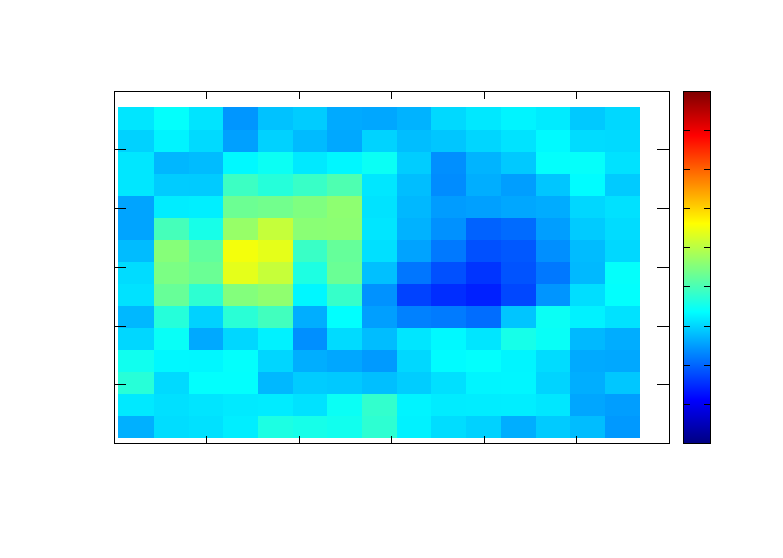
\includegraphics{plots/2DMRI200}}%
    \gplfronttext
  \end{picture}%
\endgroup

    \caption{2D MRI mit T2 $\SI{200}{\milli\second}$}
\end{figure}
\begin{figure}[H]
    \centering
    % GNUPLOT: LaTeX picture with Postscript
\begingroup
  % Encoding inside the plot.  In the header of your document, this encoding
  % should to defined, e.g., by using
  % \usepackage[cp1252,<other encodings>]{inputenc}
  \inputencoding{cp1252}%
  \makeatletter
  \providecommand\color[2][]{%
    \GenericError{(gnuplot) \space\space\space\@spaces}{%
      Package color not loaded in conjunction with
      terminal option `colourtext'%
    }{See the gnuplot documentation for explanation.%
    }{Either use 'blacktext' in gnuplot or load the package
      color.sty in LaTeX.}%
    \renewcommand\color[2][]{}%
  }%
  \providecommand\includegraphics[2][]{%
    \GenericError{(gnuplot) \space\space\space\@spaces}{%
      Package graphicx or graphics not loaded%
    }{See the gnuplot documentation for explanation.%
    }{The gnuplot epslatex terminal needs graphicx.sty or graphics.sty.}%
    \renewcommand\includegraphics[2][]{}%
  }%
  \providecommand\rotatebox[2]{#2}%
  \@ifundefined{ifGPcolor}{%
    \newif\ifGPcolor
    \GPcolorfalse
  }{}%
  \@ifundefined{ifGPblacktext}{%
    \newif\ifGPblacktext
    \GPblacktexttrue
  }{}%
  % define a \g@addto@macro without @ in the name:
  \let\gplgaddtomacro\g@addto@macro
  % define empty templates for all commands taking text:
  \gdef\gplbacktext{}%
  \gdef\gplfronttext{}%
  \makeatother
  \ifGPblacktext
    % no textcolor at all
    \def\colorrgb#1{}%
    \def\colorgray#1{}%
  \else
    % gray or color?
    \ifGPcolor
      \def\colorrgb#1{\color[rgb]{#1}}%
      \def\colorgray#1{\color[gray]{#1}}%
      \expandafter\def\csname LTw\endcsname{\color{white}}%
      \expandafter\def\csname LTb\endcsname{\color{black}}%
      \expandafter\def\csname LTa\endcsname{\color{black}}%
      \expandafter\def\csname LT0\endcsname{\color[rgb]{1,0,0}}%
      \expandafter\def\csname LT1\endcsname{\color[rgb]{0,1,0}}%
      \expandafter\def\csname LT2\endcsname{\color[rgb]{0,0,1}}%
      \expandafter\def\csname LT3\endcsname{\color[rgb]{1,0,1}}%
      \expandafter\def\csname LT4\endcsname{\color[rgb]{0,1,1}}%
      \expandafter\def\csname LT5\endcsname{\color[rgb]{1,1,0}}%
      \expandafter\def\csname LT6\endcsname{\color[rgb]{0,0,0}}%
      \expandafter\def\csname LT7\endcsname{\color[rgb]{1,0.3,0}}%
      \expandafter\def\csname LT8\endcsname{\color[rgb]{0.5,0.5,0.5}}%
    \else
      % gray
      \def\colorrgb#1{\color{black}}%
      \def\colorgray#1{\color[gray]{#1}}%
      \expandafter\def\csname LTw\endcsname{\color{white}}%
      \expandafter\def\csname LTb\endcsname{\color{black}}%
      \expandafter\def\csname LTa\endcsname{\color{black}}%
      \expandafter\def\csname LT0\endcsname{\color{black}}%
      \expandafter\def\csname LT1\endcsname{\color{black}}%
      \expandafter\def\csname LT2\endcsname{\color{black}}%
      \expandafter\def\csname LT3\endcsname{\color{black}}%
      \expandafter\def\csname LT4\endcsname{\color{black}}%
      \expandafter\def\csname LT5\endcsname{\color{black}}%
      \expandafter\def\csname LT6\endcsname{\color{black}}%
      \expandafter\def\csname LT7\endcsname{\color{black}}%
      \expandafter\def\csname LT8\endcsname{\color{black}}%
    \fi
  \fi
    \setlength{\unitlength}{0.0500bp}%
    \ifx\gptboxheight\undefined%
      \newlength{\gptboxheight}%
      \newlength{\gptboxwidth}%
      \newsavebox{\gptboxtext}%
    \fi%
    \setlength{\fboxrule}{0.5pt}%
    \setlength{\fboxsep}{1pt}%
\begin{picture}(7200.00,5040.00)%
    \gplgaddtomacro\gplbacktext{%
    }%
    \gplgaddtomacro\gplfronttext{%
      \csname LTb\endcsname%%
      \put(936,688){\makebox(0,0){\strut{}$0$}}%
      \put(1824,688){\makebox(0,0){\strut{}$20$}}%
      \put(2712,688){\makebox(0,0){\strut{}$40$}}%
      \put(3600,688){\makebox(0,0){\strut{}$60$}}%
      \put(4488,688){\makebox(0,0){\strut{}$80$}}%
      \put(5376,688){\makebox(0,0){\strut{}$100$}}%
      \put(6264,688){\makebox(0,0){\strut{}$120$}}%
      \put(3600,358){\makebox(0,0){\strut{}Y in $\si{\milli \meter}$}}%
      \put(700,938){\makebox(0,0)[r]{\strut{}$0$}}%
      \put(700,1502){\makebox(0,0)[r]{\strut{}$20$}}%
      \put(700,2066){\makebox(0,0)[r]{\strut{}$40$}}%
      \put(700,2630){\makebox(0,0)[r]{\strut{}$60$}}%
      \put(700,3194){\makebox(0,0)[r]{\strut{}$80$}}%
      \put(700,3758){\makebox(0,0)[r]{\strut{}$100$}}%
      \put(700,4322){\makebox(0,0)[r]{\strut{}$120$}}%
      \put(238,2630){\rotatebox{-270}{\makebox(0,0){\strut{}Z in $\si{\milli \meter}$}}}%
      \put(6795,938){\makebox(0,0)[l]{\strut{}$0$}}%
      \put(6795,1421){\makebox(0,0)[l]{\strut{}$10000$}}%
      \put(6795,1904){\makebox(0,0)[l]{\strut{}$20000$}}%
      \put(6795,2388){\makebox(0,0)[l]{\strut{}$30000$}}%
      \put(6795,2871){\makebox(0,0)[l]{\strut{}$40000$}}%
      \put(6795,3355){\makebox(0,0)[l]{\strut{}$50000$}}%
      \put(6795,3838){\makebox(0,0)[l]{\strut{}$60000$}}%
      \put(6795,4322){\makebox(0,0)[l]{\strut{}$70000$}}%
    }%
    \gplbacktext
    \put(0,0){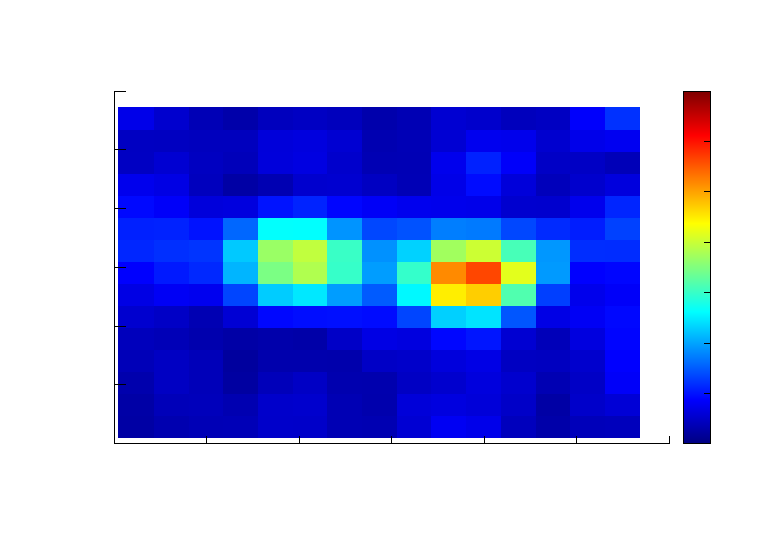
\includegraphics{plots/2DMRI250}}%
    \gplfronttext
  \end{picture}%
\endgroup

    \caption{2D MRI mit T2 $\SI{250}{\milli\second}$}
\end{figure}
\begin{figure}[H]
    \centering
    % GNUPLOT: LaTeX picture with Postscript
\begingroup
  % Encoding inside the plot.  In the header of your document, this encoding
  % should to defined, e.g., by using
  % \usepackage[cp1252,<other encodings>]{inputenc}
  \inputencoding{cp1252}%
  \makeatletter
  \providecommand\color[2][]{%
    \GenericError{(gnuplot) \space\space\space\@spaces}{%
      Package color not loaded in conjunction with
      terminal option `colourtext'%
    }{See the gnuplot documentation for explanation.%
    }{Either use 'blacktext' in gnuplot or load the package
      color.sty in LaTeX.}%
    \renewcommand\color[2][]{}%
  }%
  \providecommand\includegraphics[2][]{%
    \GenericError{(gnuplot) \space\space\space\@spaces}{%
      Package graphicx or graphics not loaded%
    }{See the gnuplot documentation for explanation.%
    }{The gnuplot epslatex terminal needs graphicx.sty or graphics.sty.}%
    \renewcommand\includegraphics[2][]{}%
  }%
  \providecommand\rotatebox[2]{#2}%
  \@ifundefined{ifGPcolor}{%
    \newif\ifGPcolor
    \GPcolorfalse
  }{}%
  \@ifundefined{ifGPblacktext}{%
    \newif\ifGPblacktext
    \GPblacktexttrue
  }{}%
  % define a \g@addto@macro without @ in the name:
  \let\gplgaddtomacro\g@addto@macro
  % define empty templates for all commands taking text:
  \gdef\gplbacktext{}%
  \gdef\gplfronttext{}%
  \makeatother
  \ifGPblacktext
    % no textcolor at all
    \def\colorrgb#1{}%
    \def\colorgray#1{}%
  \else
    % gray or color?
    \ifGPcolor
      \def\colorrgb#1{\color[rgb]{#1}}%
      \def\colorgray#1{\color[gray]{#1}}%
      \expandafter\def\csname LTw\endcsname{\color{white}}%
      \expandafter\def\csname LTb\endcsname{\color{black}}%
      \expandafter\def\csname LTa\endcsname{\color{black}}%
      \expandafter\def\csname LT0\endcsname{\color[rgb]{1,0,0}}%
      \expandafter\def\csname LT1\endcsname{\color[rgb]{0,1,0}}%
      \expandafter\def\csname LT2\endcsname{\color[rgb]{0,0,1}}%
      \expandafter\def\csname LT3\endcsname{\color[rgb]{1,0,1}}%
      \expandafter\def\csname LT4\endcsname{\color[rgb]{0,1,1}}%
      \expandafter\def\csname LT5\endcsname{\color[rgb]{1,1,0}}%
      \expandafter\def\csname LT6\endcsname{\color[rgb]{0,0,0}}%
      \expandafter\def\csname LT7\endcsname{\color[rgb]{1,0.3,0}}%
      \expandafter\def\csname LT8\endcsname{\color[rgb]{0.5,0.5,0.5}}%
    \else
      % gray
      \def\colorrgb#1{\color{black}}%
      \def\colorgray#1{\color[gray]{#1}}%
      \expandafter\def\csname LTw\endcsname{\color{white}}%
      \expandafter\def\csname LTb\endcsname{\color{black}}%
      \expandafter\def\csname LTa\endcsname{\color{black}}%
      \expandafter\def\csname LT0\endcsname{\color{black}}%
      \expandafter\def\csname LT1\endcsname{\color{black}}%
      \expandafter\def\csname LT2\endcsname{\color{black}}%
      \expandafter\def\csname LT3\endcsname{\color{black}}%
      \expandafter\def\csname LT4\endcsname{\color{black}}%
      \expandafter\def\csname LT5\endcsname{\color{black}}%
      \expandafter\def\csname LT6\endcsname{\color{black}}%
      \expandafter\def\csname LT7\endcsname{\color{black}}%
      \expandafter\def\csname LT8\endcsname{\color{black}}%
    \fi
  \fi
    \setlength{\unitlength}{0.0500bp}%
    \ifx\gptboxheight\undefined%
      \newlength{\gptboxheight}%
      \newlength{\gptboxwidth}%
      \newsavebox{\gptboxtext}%
    \fi%
    \setlength{\fboxrule}{0.5pt}%
    \setlength{\fboxsep}{1pt}%
\begin{picture}(7200.00,5040.00)%
    \gplgaddtomacro\gplbacktext{%
    }%
    \gplgaddtomacro\gplfronttext{%
      \csname LTb\endcsname%%
      \put(936,688){\makebox(0,0){\strut{}$0$}}%
      \put(1824,688){\makebox(0,0){\strut{}$20$}}%
      \put(2712,688){\makebox(0,0){\strut{}$40$}}%
      \put(3600,688){\makebox(0,0){\strut{}$60$}}%
      \put(4488,688){\makebox(0,0){\strut{}$80$}}%
      \put(5376,688){\makebox(0,0){\strut{}$100$}}%
      \put(6264,688){\makebox(0,0){\strut{}$120$}}%
      \put(3600,358){\makebox(0,0){\strut{}Y in $\si{\milli \meter}$}}%
      \put(700,938){\makebox(0,0)[r]{\strut{}$0$}}%
      \put(700,1502){\makebox(0,0)[r]{\strut{}$20$}}%
      \put(700,2066){\makebox(0,0)[r]{\strut{}$40$}}%
      \put(700,2630){\makebox(0,0)[r]{\strut{}$60$}}%
      \put(700,3194){\makebox(0,0)[r]{\strut{}$80$}}%
      \put(700,3758){\makebox(0,0)[r]{\strut{}$100$}}%
      \put(700,4322){\makebox(0,0)[r]{\strut{}$120$}}%
      \put(238,2630){\rotatebox{-270}{\makebox(0,0){\strut{}Z in $\si{\milli \meter}$}}}%
      \put(6795,938){\makebox(0,0)[l]{\strut{}$0$}}%
      \put(6795,1421){\makebox(0,0)[l]{\strut{}$10000$}}%
      \put(6795,1904){\makebox(0,0)[l]{\strut{}$20000$}}%
      \put(6795,2388){\makebox(0,0)[l]{\strut{}$30000$}}%
      \put(6795,2871){\makebox(0,0)[l]{\strut{}$40000$}}%
      \put(6795,3355){\makebox(0,0)[l]{\strut{}$50000$}}%
      \put(6795,3838){\makebox(0,0)[l]{\strut{}$60000$}}%
      \put(6795,4322){\makebox(0,0)[l]{\strut{}$70000$}}%
    }%
    \gplbacktext
    \put(0,0){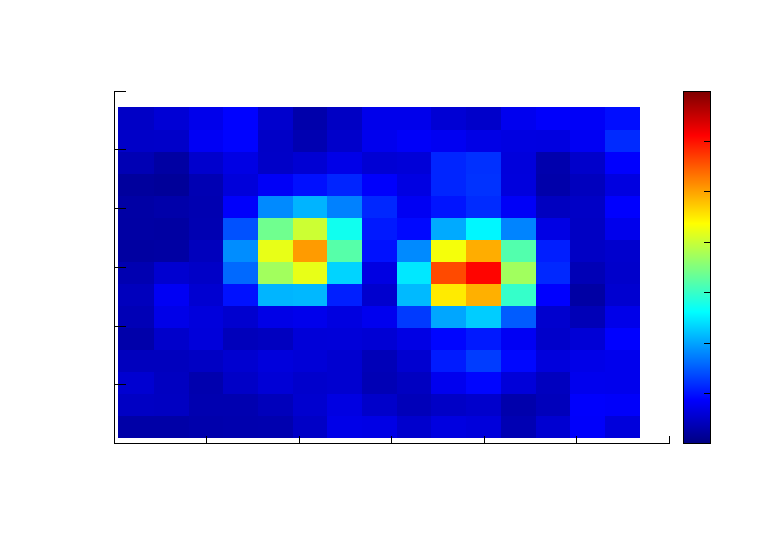
\includegraphics{plots/2DMRI300}}%
    \gplfronttext
  \end{picture}%
\endgroup

    \caption{2D MRI mit T2 $\SI{300}{\milli\second}$}
\end{figure}
\begin{figure}[H]
    \centering
    % GNUPLOT: LaTeX picture with Postscript
\begingroup
  % Encoding inside the plot.  In the header of your document, this encoding
  % should to defined, e.g., by using
  % \usepackage[cp1252,<other encodings>]{inputenc}
  \inputencoding{cp1252}%
  \makeatletter
  \providecommand\color[2][]{%
    \GenericError{(gnuplot) \space\space\space\@spaces}{%
      Package color not loaded in conjunction with
      terminal option `colourtext'%
    }{See the gnuplot documentation for explanation.%
    }{Either use 'blacktext' in gnuplot or load the package
      color.sty in LaTeX.}%
    \renewcommand\color[2][]{}%
  }%
  \providecommand\includegraphics[2][]{%
    \GenericError{(gnuplot) \space\space\space\@spaces}{%
      Package graphicx or graphics not loaded%
    }{See the gnuplot documentation for explanation.%
    }{The gnuplot epslatex terminal needs graphicx.sty or graphics.sty.}%
    \renewcommand\includegraphics[2][]{}%
  }%
  \providecommand\rotatebox[2]{#2}%
  \@ifundefined{ifGPcolor}{%
    \newif\ifGPcolor
    \GPcolorfalse
  }{}%
  \@ifundefined{ifGPblacktext}{%
    \newif\ifGPblacktext
    \GPblacktexttrue
  }{}%
  % define a \g@addto@macro without @ in the name:
  \let\gplgaddtomacro\g@addto@macro
  % define empty templates for all commands taking text:
  \gdef\gplbacktext{}%
  \gdef\gplfronttext{}%
  \makeatother
  \ifGPblacktext
    % no textcolor at all
    \def\colorrgb#1{}%
    \def\colorgray#1{}%
  \else
    % gray or color?
    \ifGPcolor
      \def\colorrgb#1{\color[rgb]{#1}}%
      \def\colorgray#1{\color[gray]{#1}}%
      \expandafter\def\csname LTw\endcsname{\color{white}}%
      \expandafter\def\csname LTb\endcsname{\color{black}}%
      \expandafter\def\csname LTa\endcsname{\color{black}}%
      \expandafter\def\csname LT0\endcsname{\color[rgb]{1,0,0}}%
      \expandafter\def\csname LT1\endcsname{\color[rgb]{0,1,0}}%
      \expandafter\def\csname LT2\endcsname{\color[rgb]{0,0,1}}%
      \expandafter\def\csname LT3\endcsname{\color[rgb]{1,0,1}}%
      \expandafter\def\csname LT4\endcsname{\color[rgb]{0,1,1}}%
      \expandafter\def\csname LT5\endcsname{\color[rgb]{1,1,0}}%
      \expandafter\def\csname LT6\endcsname{\color[rgb]{0,0,0}}%
      \expandafter\def\csname LT7\endcsname{\color[rgb]{1,0.3,0}}%
      \expandafter\def\csname LT8\endcsname{\color[rgb]{0.5,0.5,0.5}}%
    \else
      % gray
      \def\colorrgb#1{\color{black}}%
      \def\colorgray#1{\color[gray]{#1}}%
      \expandafter\def\csname LTw\endcsname{\color{white}}%
      \expandafter\def\csname LTb\endcsname{\color{black}}%
      \expandafter\def\csname LTa\endcsname{\color{black}}%
      \expandafter\def\csname LT0\endcsname{\color{black}}%
      \expandafter\def\csname LT1\endcsname{\color{black}}%
      \expandafter\def\csname LT2\endcsname{\color{black}}%
      \expandafter\def\csname LT3\endcsname{\color{black}}%
      \expandafter\def\csname LT4\endcsname{\color{black}}%
      \expandafter\def\csname LT5\endcsname{\color{black}}%
      \expandafter\def\csname LT6\endcsname{\color{black}}%
      \expandafter\def\csname LT7\endcsname{\color{black}}%
      \expandafter\def\csname LT8\endcsname{\color{black}}%
    \fi
  \fi
    \setlength{\unitlength}{0.0500bp}%
    \ifx\gptboxheight\undefined%
      \newlength{\gptboxheight}%
      \newlength{\gptboxwidth}%
      \newsavebox{\gptboxtext}%
    \fi%
    \setlength{\fboxrule}{0.5pt}%
    \setlength{\fboxsep}{1pt}%
\begin{picture}(7200.00,5040.00)%
    \gplgaddtomacro\gplbacktext{%
    }%
    \gplgaddtomacro\gplfronttext{%
      \csname LTb\endcsname%%
      \put(936,688){\makebox(0,0){\strut{}$0$}}%
      \put(1824,688){\makebox(0,0){\strut{}$20$}}%
      \put(2712,688){\makebox(0,0){\strut{}$40$}}%
      \put(3600,688){\makebox(0,0){\strut{}$60$}}%
      \put(4488,688){\makebox(0,0){\strut{}$80$}}%
      \put(5376,688){\makebox(0,0){\strut{}$100$}}%
      \put(6264,688){\makebox(0,0){\strut{}$120$}}%
      \put(3600,358){\makebox(0,0){\strut{}Y in $\si{\milli \meter}$}}%
      \put(700,938){\makebox(0,0)[r]{\strut{}$0$}}%
      \put(700,1502){\makebox(0,0)[r]{\strut{}$20$}}%
      \put(700,2066){\makebox(0,0)[r]{\strut{}$40$}}%
      \put(700,2630){\makebox(0,0)[r]{\strut{}$60$}}%
      \put(700,3194){\makebox(0,0)[r]{\strut{}$80$}}%
      \put(700,3758){\makebox(0,0)[r]{\strut{}$100$}}%
      \put(700,4322){\makebox(0,0)[r]{\strut{}$120$}}%
      \put(238,2630){\rotatebox{-270}{\makebox(0,0){\strut{}Z in $\si{\milli \meter}$}}}%
      \put(6795,938){\makebox(0,0)[l]{\strut{}$0$}}%
      \put(6795,1314){\makebox(0,0)[l]{\strut{}$5000$}}%
      \put(6795,1690){\makebox(0,0)[l]{\strut{}$10000$}}%
      \put(6795,2066){\makebox(0,0)[l]{\strut{}$15000$}}%
      \put(6795,2442){\makebox(0,0)[l]{\strut{}$20000$}}%
      \put(6795,2818){\makebox(0,0)[l]{\strut{}$25000$}}%
      \put(6795,3194){\makebox(0,0)[l]{\strut{}$30000$}}%
      \put(6795,3570){\makebox(0,0)[l]{\strut{}$35000$}}%
      \put(6795,3946){\makebox(0,0)[l]{\strut{}$40000$}}%
      \put(6795,4322){\makebox(0,0)[l]{\strut{}$45000$}}%
    }%
    \gplbacktext
    \put(0,0){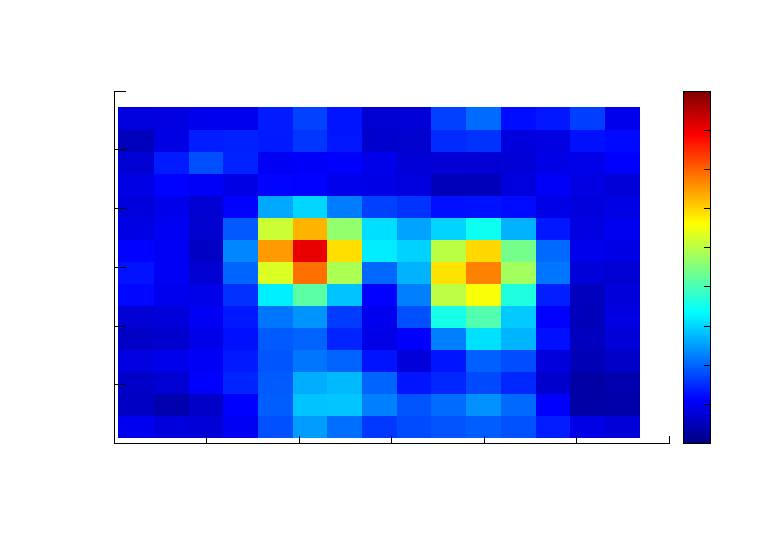
\includegraphics{plots/2DMRI450}}%
    \gplfronttext
  \end{picture}%
\endgroup

    \caption{2D MRI mit T2 $\SI{450}{\milli\second}$}
\end{figure}
\begin{figure}[H]
    \centering
    % GNUPLOT: LaTeX picture with Postscript
\begingroup
  % Encoding inside the plot.  In the header of your document, this encoding
  % should to defined, e.g., by using
  % \usepackage[cp1252,<other encodings>]{inputenc}
  \inputencoding{cp1252}%
  \makeatletter
  \providecommand\color[2][]{%
    \GenericError{(gnuplot) \space\space\space\@spaces}{%
      Package color not loaded in conjunction with
      terminal option `colourtext'%
    }{See the gnuplot documentation for explanation.%
    }{Either use 'blacktext' in gnuplot or load the package
      color.sty in LaTeX.}%
    \renewcommand\color[2][]{}%
  }%
  \providecommand\includegraphics[2][]{%
    \GenericError{(gnuplot) \space\space\space\@spaces}{%
      Package graphicx or graphics not loaded%
    }{See the gnuplot documentation for explanation.%
    }{The gnuplot epslatex terminal needs graphicx.sty or graphics.sty.}%
    \renewcommand\includegraphics[2][]{}%
  }%
  \providecommand\rotatebox[2]{#2}%
  \@ifundefined{ifGPcolor}{%
    \newif\ifGPcolor
    \GPcolorfalse
  }{}%
  \@ifundefined{ifGPblacktext}{%
    \newif\ifGPblacktext
    \GPblacktexttrue
  }{}%
  % define a \g@addto@macro without @ in the name:
  \let\gplgaddtomacro\g@addto@macro
  % define empty templates for all commands taking text:
  \gdef\gplbacktext{}%
  \gdef\gplfronttext{}%
  \makeatother
  \ifGPblacktext
    % no textcolor at all
    \def\colorrgb#1{}%
    \def\colorgray#1{}%
  \else
    % gray or color?
    \ifGPcolor
      \def\colorrgb#1{\color[rgb]{#1}}%
      \def\colorgray#1{\color[gray]{#1}}%
      \expandafter\def\csname LTw\endcsname{\color{white}}%
      \expandafter\def\csname LTb\endcsname{\color{black}}%
      \expandafter\def\csname LTa\endcsname{\color{black}}%
      \expandafter\def\csname LT0\endcsname{\color[rgb]{1,0,0}}%
      \expandafter\def\csname LT1\endcsname{\color[rgb]{0,1,0}}%
      \expandafter\def\csname LT2\endcsname{\color[rgb]{0,0,1}}%
      \expandafter\def\csname LT3\endcsname{\color[rgb]{1,0,1}}%
      \expandafter\def\csname LT4\endcsname{\color[rgb]{0,1,1}}%
      \expandafter\def\csname LT5\endcsname{\color[rgb]{1,1,0}}%
      \expandafter\def\csname LT6\endcsname{\color[rgb]{0,0,0}}%
      \expandafter\def\csname LT7\endcsname{\color[rgb]{1,0.3,0}}%
      \expandafter\def\csname LT8\endcsname{\color[rgb]{0.5,0.5,0.5}}%
    \else
      % gray
      \def\colorrgb#1{\color{black}}%
      \def\colorgray#1{\color[gray]{#1}}%
      \expandafter\def\csname LTw\endcsname{\color{white}}%
      \expandafter\def\csname LTb\endcsname{\color{black}}%
      \expandafter\def\csname LTa\endcsname{\color{black}}%
      \expandafter\def\csname LT0\endcsname{\color{black}}%
      \expandafter\def\csname LT1\endcsname{\color{black}}%
      \expandafter\def\csname LT2\endcsname{\color{black}}%
      \expandafter\def\csname LT3\endcsname{\color{black}}%
      \expandafter\def\csname LT4\endcsname{\color{black}}%
      \expandafter\def\csname LT5\endcsname{\color{black}}%
      \expandafter\def\csname LT6\endcsname{\color{black}}%
      \expandafter\def\csname LT7\endcsname{\color{black}}%
      \expandafter\def\csname LT8\endcsname{\color{black}}%
    \fi
  \fi
    \setlength{\unitlength}{0.0500bp}%
    \ifx\gptboxheight\undefined%
      \newlength{\gptboxheight}%
      \newlength{\gptboxwidth}%
      \newsavebox{\gptboxtext}%
    \fi%
    \setlength{\fboxrule}{0.5pt}%
    \setlength{\fboxsep}{1pt}%
\begin{picture}(7200.00,5040.00)%
    \gplgaddtomacro\gplbacktext{%
    }%
    \gplgaddtomacro\gplfronttext{%
      \csname LTb\endcsname%%
      \put(936,688){\makebox(0,0){\strut{}$0$}}%
      \put(1824,688){\makebox(0,0){\strut{}$20$}}%
      \put(2712,688){\makebox(0,0){\strut{}$40$}}%
      \put(3600,688){\makebox(0,0){\strut{}$60$}}%
      \put(4488,688){\makebox(0,0){\strut{}$80$}}%
      \put(5376,688){\makebox(0,0){\strut{}$100$}}%
      \put(6264,688){\makebox(0,0){\strut{}$120$}}%
      \put(3600,358){\makebox(0,0){\strut{}Y in $\si{\milli \meter}$}}%
      \put(700,938){\makebox(0,0)[r]{\strut{}$0$}}%
      \put(700,1502){\makebox(0,0)[r]{\strut{}$20$}}%
      \put(700,2066){\makebox(0,0)[r]{\strut{}$40$}}%
      \put(700,2630){\makebox(0,0)[r]{\strut{}$60$}}%
      \put(700,3194){\makebox(0,0)[r]{\strut{}$80$}}%
      \put(700,3758){\makebox(0,0)[r]{\strut{}$100$}}%
      \put(700,4322){\makebox(0,0)[r]{\strut{}$120$}}%
      \put(238,2630){\rotatebox{-270}{\makebox(0,0){\strut{}Z in $\si{\milli \meter}$}}}%
      \put(6795,938){\makebox(0,0)[l]{\strut{}$0$}}%
      \put(6795,1314){\makebox(0,0)[l]{\strut{}$5000$}}%
      \put(6795,1690){\makebox(0,0)[l]{\strut{}$10000$}}%
      \put(6795,2066){\makebox(0,0)[l]{\strut{}$15000$}}%
      \put(6795,2442){\makebox(0,0)[l]{\strut{}$20000$}}%
      \put(6795,2818){\makebox(0,0)[l]{\strut{}$25000$}}%
      \put(6795,3194){\makebox(0,0)[l]{\strut{}$30000$}}%
      \put(6795,3570){\makebox(0,0)[l]{\strut{}$35000$}}%
      \put(6795,3946){\makebox(0,0)[l]{\strut{}$40000$}}%
      \put(6795,4322){\makebox(0,0)[l]{\strut{}$45000$}}%
    }%
    \gplbacktext
    \put(0,0){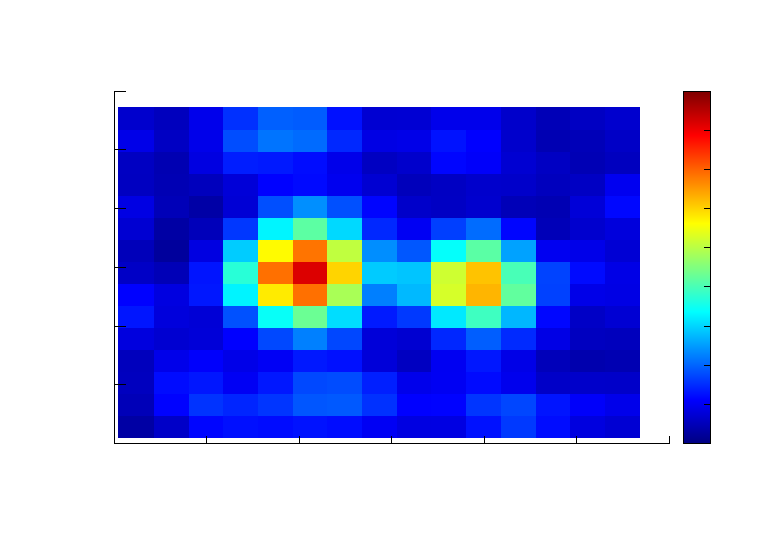
\includegraphics{plots/2DMRI550}}%
    \gplfronttext
  \end{picture}%
\endgroup

    \caption{2D MRI mit T2 $\SI{550}{\milli\second}$}
\end{figure}
% GNUPLOT: LaTeX picture with Postscript
\begingroup
  % Encoding inside the plot.  In the header of your document, this encoding
  % should to defined, e.g., by using
  % \usepackage[cp1252,<other encodings>]{inputenc}
  \inputencoding{cp1252}%
  \makeatletter
  \providecommand\color[2][]{%
    \GenericError{(gnuplot) \space\space\space\@spaces}{%
      Package color not loaded in conjunction with
      terminal option `colourtext'%
    }{See the gnuplot documentation for explanation.%
    }{Either use 'blacktext' in gnuplot or load the package
      color.sty in LaTeX.}%
    \renewcommand\color[2][]{}%
  }%
  \providecommand\includegraphics[2][]{%
    \GenericError{(gnuplot) \space\space\space\@spaces}{%
      Package graphicx or graphics not loaded%
    }{See the gnuplot documentation for explanation.%
    }{The gnuplot epslatex terminal needs graphicx.sty or graphics.sty.}%
    \renewcommand\includegraphics[2][]{}%
  }%
  \providecommand\rotatebox[2]{#2}%
  \@ifundefined{ifGPcolor}{%
    \newif\ifGPcolor
    \GPcolorfalse
  }{}%
  \@ifundefined{ifGPblacktext}{%
    \newif\ifGPblacktext
    \GPblacktexttrue
  }{}%
  % define a \g@addto@macro without @ in the name:
  \let\gplgaddtomacro\g@addto@macro
  % define empty templates for all commands taking text:
  \gdef\gplbacktext{}%
  \gdef\gplfronttext{}%
  \makeatother
  \ifGPblacktext
    % no textcolor at all
    \def\colorrgb#1{}%
    \def\colorgray#1{}%
  \else
    % gray or color?
    \ifGPcolor
      \def\colorrgb#1{\color[rgb]{#1}}%
      \def\colorgray#1{\color[gray]{#1}}%
      \expandafter\def\csname LTw\endcsname{\color{white}}%
      \expandafter\def\csname LTb\endcsname{\color{black}}%
      \expandafter\def\csname LTa\endcsname{\color{black}}%
      \expandafter\def\csname LT0\endcsname{\color[rgb]{1,0,0}}%
      \expandafter\def\csname LT1\endcsname{\color[rgb]{0,1,0}}%
      \expandafter\def\csname LT2\endcsname{\color[rgb]{0,0,1}}%
      \expandafter\def\csname LT3\endcsname{\color[rgb]{1,0,1}}%
      \expandafter\def\csname LT4\endcsname{\color[rgb]{0,1,1}}%
      \expandafter\def\csname LT5\endcsname{\color[rgb]{1,1,0}}%
      \expandafter\def\csname LT6\endcsname{\color[rgb]{0,0,0}}%
      \expandafter\def\csname LT7\endcsname{\color[rgb]{1,0.3,0}}%
      \expandafter\def\csname LT8\endcsname{\color[rgb]{0.5,0.5,0.5}}%
    \else
      % gray
      \def\colorrgb#1{\color{black}}%
      \def\colorgray#1{\color[gray]{#1}}%
      \expandafter\def\csname LTw\endcsname{\color{white}}%
      \expandafter\def\csname LTb\endcsname{\color{black}}%
      \expandafter\def\csname LTa\endcsname{\color{black}}%
      \expandafter\def\csname LT0\endcsname{\color{black}}%
      \expandafter\def\csname LT1\endcsname{\color{black}}%
      \expandafter\def\csname LT2\endcsname{\color{black}}%
      \expandafter\def\csname LT3\endcsname{\color{black}}%
      \expandafter\def\csname LT4\endcsname{\color{black}}%
      \expandafter\def\csname LT5\endcsname{\color{black}}%
      \expandafter\def\csname LT6\endcsname{\color{black}}%
      \expandafter\def\csname LT7\endcsname{\color{black}}%
      \expandafter\def\csname LT8\endcsname{\color{black}}%
    \fi
  \fi
    \setlength{\unitlength}{0.0500bp}%
    \ifx\gptboxheight\undefined%
      \newlength{\gptboxheight}%
      \newlength{\gptboxwidth}%
      \newsavebox{\gptboxtext}%
    \fi%
    \setlength{\fboxrule}{0.5pt}%
    \setlength{\fboxsep}{1pt}%
\begin{picture}(7200.00,5040.00)%
    \gplgaddtomacro\gplbacktext{%
      \csname LTb\endcsname%%
      \put(814,704){\makebox(0,0)[r]{\strut{}$0.1$}}%
      \put(814,1943){\makebox(0,0)[r]{\strut{}$0.2$}}%
      \put(814,2667){\makebox(0,0)[r]{\strut{}$0.3$}}%
      \put(814,3181){\makebox(0,0)[r]{\strut{}$0.4$}}%
      \put(814,3580){\makebox(0,0)[r]{\strut{}$0.5$}}%
      \put(814,3906){\makebox(0,0)[r]{\strut{}$0.6$}}%
      \put(814,4182){\makebox(0,0)[r]{\strut{}$0.7$}}%
      \put(814,4420){\makebox(0,0)[r]{\strut{}$0.8$}}%
      \put(814,4631){\makebox(0,0)[r]{\strut{}$0.9$}}%
      \put(814,4819){\makebox(0,0)[r]{\strut{}$1$}}%
      \put(946,484){\makebox(0,0){\strut{}$0$}}%
      \put(1922,484){\makebox(0,0){\strut{}$1\times10^{8}$}}%
      \put(2898,484){\makebox(0,0){\strut{}$2\times10^{8}$}}%
      \put(3875,484){\makebox(0,0){\strut{}$3\times10^{8}$}}%
      \put(4851,484){\makebox(0,0){\strut{}$4\times10^{8}$}}%
      \put(5827,484){\makebox(0,0){\strut{}$5\times10^{8}$}}%
      \put(6803,484){\makebox(0,0){\strut{}$6\times10^{8}$}}%
    }%
    \gplgaddtomacro\gplfronttext{%
      \csname LTb\endcsname%%
      \put(198,2761){\rotatebox{-270}{\makebox(0,0){\strut{}Abd\"ampfung $\frac{E}{E_0}$}}}%
      \put(3874,154){\makebox(0,0){\strut{}$\gamma^2 G^2 \delta^2 (\Delta-\frac{\delta}{3})$$\left[\frac{\si{\s}}{\si{\m^2}}\right]$}}%
      \csname LTb\endcsname%%
      \put(5816,4646){\makebox(0,0)[r]{\strut{}Polarisationszeit $\SI{4}{\second}$}}%
      \csname LTb\endcsname%%
      \put(5816,4426){\makebox(0,0)[r]{\strut{}Exponentieller-Fit}}%
    }%
    \gplbacktext
    \put(0,0){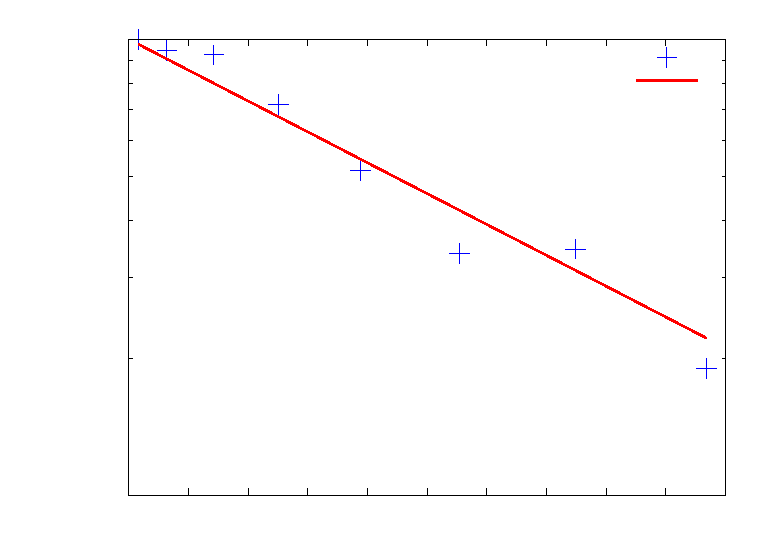
\includegraphics{plots/Diffusion}}%
    \gplfronttext
  \end{picture}%
\endgroup

%----------------------------------------------------------------%
%----------------------Fazit-------------------------------------%
%----------------------------------------------------------------%
\newpage
% !TEX root = main.tex
\section{Fehlerdiskussion und Fazit}
In Bezug auf die Beobachtung der Sonne kann ein durchweg positives Fazit gezogen werden.
Einige Annahmen -- die Sonne als Punktquelle oder das Teleskop als Lochblende aufzufassen -- und daran anknüpfende Folgerungen, wie das Erhalten der $\sinc$-Funktion oder das Berechnen des Auflösungsvermögens mittels FWHM wurden durch die guten Ergebnisse und anschaulichen Grafiken legitimiert.
Bis auf die Positioniergenauigkeit -- $\SI{0.976 \pm 0.034}{\degree}$ gegenüber $\SI{0.5}{\degree}$ \cite{Usermanual} -- und den beiden Durchmessern -- $D_{\text{az}} = \SI{1.895 \pm 0.032}{\metre}$ und $D_{\text{alt}} = \SI{2.625 \pm 0.056}{\metre}$ gegnüber $D = \SI{2.3}{\metre}$ \cite{Usermanual} -- des Teleskops liegen alle ermittelten Charakteristika auf Grundlage der Unsicherheiten in guter Übereinstimmung mit den Werten der Projekt-Dokumentation \cite{Usermanual}.
Auch die Positioniergenauigkeit liegt in derselben Größenordnung und widerspricht somit nicht gänzlich der Erwartung.
Das Auflösungsvermögen ($\SI{6.6 \pm 1.1}{\degree}$ zu $\SI{6}{\degree}$ \cite{Usermanual}) und das Rückrechnen auf den Mittelwert des Teleskopdurchmessers ($\SI{2.23 \pm 0.37}{\metre}$ zu $\SI{2.3}{\metre}$ \cite{Usermanual}) zeigen wie erwähnt gute Übereinstimmungen.

Die Unsicherheiten der betrachteten Werte liegen allesamt in sinnvollen Größenordnungen und lassen darauf schließen, dass kein systematischer Fehler während der Durchführung und Auswertung des Versuchs auftrat und auch mögliche Defekte oder äußere Einflüsse keine zu große Beeinträchtigung der Messung darstellten.
Auffällig war, dass stets bei der Variation des Höhenversatzwinkels schmalere $\sinc$-Profile respektive \textSC{Gauss}-Kurven auftraten.
Hierfür wurden verschiedene Ansätze diskutiert.
Zum einen wurden Witterung und äußere Verhältnisse am Versuchstag in Erwägung gezogen.
Da das Teleskop allerdings in verschiedenen Ausrichtungen Messungen vornahm, könnte ein stets aus einer Richtung wehender Wind zwar Einfluss auf die Positioniergenauigkeit haben, aber keine solche kontinuierlich auftretende Abweichung erklären.
Eventuell vorliegende Defekte des Parabolspiegels, welche den effektiven Beitrag bestimmter Teleskopareale zur Messung schmälern, sowie daraus resultierende Abweichungen der Justierung oder Schäden der Mechanik des Teleskops sind hierbei deutlich plausiblere Fehlerquellen.
Mögliche Verbesserungen hinsichtlich der Messgenauigkeit könnten durch eine größere Zahl Messungen oder beispielsweise kleinschrittigere Variation der Versatzwinkel in Azimut und Höhenkomponente erreicht werden.
Die Defekte am Teleskop könnten durch regelmäßigere Wartungen minimiert werden.
Zudem könnten diese bei der Justierung berücksichtigt werden, um die Messergebnisse zu verbessern. \newpage

Auch die Messungen und Berechnungen der Milchstraße lieferten sehr gute Werte, welche stets in guter Übereinstimmung mit der Literatur sind. 
Ausschlaggebende erfolgsfaktoren dieses Versuchsteils sind zum einen die nahezu konstante Geschwindigkeit der Körper in der Milchstraße von $\SI{210.9 \pm 3.1}{\frac{km}{s}}$ (Literaturwert $\SI{220}{\frac{km}{s}}$ \cite{LSR}), was deutlich auf eine unbekannte Energie und Materie im Universum hindeutet, zum anderen die sehr präzise Kartografie der Milchstraße.
Hier sind die Seitenarme \textit{Cygnus}, \textit{Perseus} und \textit{Orion} anhand eines Vergleichs mit der Literatur bestimmbar.
Somit war ein hinreichend präzises Vermessen der Milchstraße gewährleistet. 
Wenn allerdings noch bessere Ergebnisse erzielt werden sollen, so müssen einige Unsicherheitsquellen und deren Folgen in Betracht gezogen werden. 
Eine Unsicherheitsquelle, welche Auswirkungen auf den gesamten Versuchsteil hat, ist die Integrationszeit der vermessenen Spektren. 
Denn wenn das Spektrum stärkeres Rauschen aufweist, so liefern die \textsc{Gauss}-Funktionen eine größere Unsicherheit und die Maxima sind schlechter auswertbar. 
Wie bereits diskutiert, verbessert sich das Rauschen des Spektrums bei längeren Integrationszeiten. 
Wenn also präzisere Messwerte erreicht werden wollen, so muss die Integrationszeit erhöht werden. 
Des Weiteren kann die konstante Geschwindigkeit der Wasserstoffwolken durch eine Ergänzung von zusätzlichen Messwerten genauer analysiert werden. 
Denn je mehr Messwerte vorhanden sind, desto genauer lässt sich ein Mittelwert ermitteln. 
Viele Messwerte sind auch für die Katografie der Milchstraße von Vorteil.
Denn somit fallen Fehlerpunkte nicht mehr so stark ins Gewicht und die Galaxiearme sind noch besser identifizierbar. \\

Trotz aller diskutierten Unsicherheiten ist dieser Versuch mit den verwendeten Parametern eine sehr gute Möglichkeit, gute Ergebnisse zu erzielen.
Wenn allerdings noch genauere Ergebnisse erreicht werden sollen, so müssen die genannten Verbesserungen bezüglich der Unsicherheiten in Betracht gezogen werden.
\newpage
%----------------------------------------------------------------%
%----------------------Verzeichnisse-----------------------------%
%----------------------------------------------------------------%
% !TEX root = main.tex
\bibliography{literatur}
\bibliographystyle{babalpha}
\newpage
\listoffigures
\listoftables
\addcontentsline{toc}{section}{Attachments}
\section*{Attachments}
\setcounter{section}{6}
\newpage


\begin{table}[H]
    \centering
    \caption{$T_1$ und $T_2$ abhängig vom Kontrastmittel und dessen Konzentration.}
    \begin{tabular}{lllll}  \hline
    \multicolumn{1}{|l||}{}            & \multicolumn{1}{l|}{T1 in \si{\milli \second}}      & \multicolumn{1}{l|}{U(T1)-Fit in \si{\milli \second}} & \multicolumn{1}{l|}{T2 in \si{\milli \second}}      & \multicolumn{1}{l|}{U(T2)-Fit in \si{\milli \second}}  \\ \hline
    \multicolumn{1}{|l||}{Wasser}      & \multicolumn{1}{l|}{2199,46} & \multicolumn{1}{l|}{0,003027}  & \multicolumn{1}{l|}{1901,06} & \multicolumn{1}{l|}{89,83}      \\ \hline \hline
    \multicolumn{1}{|l||}{\ce{Cu^2+}    ($\SI{0.5}{\frac{\mol}{\metre \tothe{3}}}$)}  & \multicolumn{1}{l|}{1394,84} & \multicolumn{1}{l|}{0,001055}  & \multicolumn{1}{l|}{1215,51} & \multicolumn{1}{l|}{0,0002529}  \\ \hline
    \multicolumn{1}{|l||}{\ce{Cu^2+}    ($\SI{1.0}{\frac{\mol}{\metre \tothe{3}}}$)}  & \multicolumn{1}{l|}{1003,4}  & \multicolumn{1}{l|}{0,0004851} & \multicolumn{1}{l|}{1066,44} & \multicolumn{1}{l|}{0,0002621}  \\ \hline
    \multicolumn{1}{|l||}{\ce{Cu^2+}    ($\SI{2.0}{\frac{\mol}{\metre \tothe{3}}}$)} & \multicolumn{1}{l|}{646,849} & \multicolumn{1}{l|}{71,54}     & \multicolumn{1}{l|}{748,404} & \multicolumn{1}{l|}{0,0001937}  \\ \hline
    \multicolumn{1}{|l||}{\ce{Cu^2+}    ($\SI{4.0}{\frac{\mol}{\metre \tothe{3}}}$)} & \multicolumn{1}{l|}{431,268} & \multicolumn{1}{l|}{0,0002906} & \multicolumn{1}{l|}{341,83}  & \multicolumn{1}{l|}{0,0001228}  \\ \hline \hline
    \multicolumn{1}{|l||}{\ce{Mn^2+}    ($\SI{0.05}{\frac{\mol}{\metre \tothe{3}}}$)}     & \multicolumn{1}{l|}{1178,28} & \multicolumn{1}{l|}{0,0009801} & \multicolumn{1}{l|}{548,337} & \multicolumn{1}{l|}{0,0001258}  \\ \hline
    \multicolumn{1}{|l||}{\ce{Mn^2+}    ($\SI{0.10}{\frac{\mol}{\metre \tothe{3}}}$)}     & \multicolumn{1}{l|}{725,857} & \multicolumn{1}{l|}{0,0006027} & \multicolumn{1}{l|}{279,858} & \multicolumn{1}{l|}{0,00008179} \\ \hline
    \multicolumn{1}{|l||}{\ce{Mn^2+}    ($\SI{0.20}{\frac{\mol}{\metre \tothe{3}}}$)}    & \multicolumn{1}{l|}{316,085} & \multicolumn{1}{l|}{0,0003079} & \multicolumn{1}{l|}{170,996} & \multicolumn{1}{l|}{0,0001182}  \\ \hline
    \multicolumn{1}{|l||}{\ce{Mn^2+}    ($\SI{0.40}{\frac{\mol}{\metre \tothe{3}}}$)}    & \multicolumn{1}{l|}{180,244} & \multicolumn{1}{l|}{0,0001274} & \multicolumn{1}{l|}{69,1512} & \multicolumn{1}{l|}{0,0000547}  \\ \hline
    \end{tabular}
    \label{tab:T1T2Kontrast}
\end{table}

\end{document}